\documentclass[11pt]{article}

\usepackage[a4paper,margin=1in]{geometry}
\usepackage[strict]{changepage}
\usepackage{booktabs, threeparttable, adjustbox, tabularx, longtable}
\usepackage{amsmath, amssymb, amsthm, bbm}
\usepackage{hyperref, achicago}
\usepackage{caption, graphicx}
\usepackage{secdot, sectsty}
\usepackage{pdflscape}
\usepackage{placeins}
\usepackage{xcolor}
\usepackage{tgschola}

\fontfamily{qcs}
\linespread{1}
\urlstyle{tt}

\allsectionsfont{\rmfamily}
\sectionfont{\normalsize}
\subsectionfont{\normalsize\selectfont}
\subsubsectionfont{\normalfont\normalsize\selectfont\itshape}

\newcommand{\specialcell}[2][c]{\begin{tabular}[#1]{@{}c@{}}#2\end{tabular}}

\begin{document}

\title{\textsc{Using Lotteries to Encourage Saving: Supplemental Appendix}\protect\footnote{For online publication only. Files for replication are available at \url{https://github.com/princetonbpl/akiba-lottery-pub}.}}

\author{Justin Abraham\thanks{Department of Economics. University of California, San Diego. \protect\href{mailto:jabraham@ucsd.edu}{\nolinkurl{jabraham@ucsd.edu}}.}, Merve Akbas\thanks{Department of Economics. Duke University. \protect\href{mailto:merve.akbas@duke.edu}{\nolinkurl{merve.akbas@duke.edu}}.}, Dan Ariely\thanks{Fuqua School of Business. Duke University. \protect\href{mailto:dan@danariely.com}{\nolinkurl{dan@danariely.com}}.}, and Chaning Jang\thanks{The Busara Center for Behavioral Economics. \protect\href{mailto:chaning.jang@busaracenter.org}{\nolinkurl{chaning.jang@busaracenter.org}}.}} % add funding statement and ethics and thanks

\maketitle

\newpage

\tableofcontents

\newpage

\appendix

\section{Experimental materials}

    % timeline
    % lab tasks
    % questionnaires
    % consent forms

    \subsection{Consent form}

        \noindent You are asked to participate in research project conducted by researchers at Duke University, Dan Ariely (dan@danariely.com) and Seher Merve Akbas (merve.akbas@duke.edu). The purpose of this project is (1) to understand how people make decisions about money, (2) how people make risky decisions, (3) how people decide to save money.

        \vspace{5mm}

        \noindent During the study in the laboratory, you will be presented a number of decisions involving money. Your payment will depend on your decisions and specific rules about it will be explained to you before you start.

        \vspace{5mm}

        \noindent Your participation in this project is completely voluntary and you are free to withdraw from it at any time.  During the project, all the information about you will be analyzed anonymously and reported by groups.

        \vspace{5mm}

        \noindent Do you have any questions that you would like to ask now?

        \vspace{5mm}

        \noindent For any future questions or concerns about the project, please contact the researcher Seher Merve Akbas via e-mail (merve.akbas@duke.edu) or phone (+1919-328-0080) or Dan Ariely via e-mail (dan@danariely.com) or the project associate, James Vancel (email: jvancel@poverty-action.org) (Phone: +254725066428), or the project manager, Joseph Njoroge (jmuiruri@poverty-action.org) (Phone: +254722900068).

        \vspace{5mm}

        \noindent I have read this information, and would like to participate

        \vspace{5mm}

        \noindent Name: \qquad Date:

    \subsection{Savings account information}

        \begin{figure}[ht]
        \centering
        \caption{Savings card for lottery group (front)}
        \includegraphics[width=0.75\textwidth]{../../figures/id_front.pdf}
        \end{figure}

        \begin{figure}[ht]
        \centering
        \caption{Savings card for lottery group (back)}
        \includegraphics[width=0.75\textwidth]{../../figures/id_back.pdf}
        \end{figure}

    \clearpage

    \subsection{Savings reminders}

        \subsubsection{Control}

            \begin{enumerate}
                \item \underline{Reminder}: ``{Name}, remember to save XX or more today to earn 1.1\% daily interest. Sambaza *140*XX*Phone to save''
                \item \underline{Upon receipt of airtime}: ``You saved XX.  You need to save YY more to receive interest. Your balance is ZZ. Keep saving with *140*XX*Phone to save''
                \item \underline{Upon receipt of sufficient airtime for match}: ``You saved XX.  You earned 1.1\% interest!  QQ was deposited into your account.  Your balance is ZZ.''
            \end{enumerate}

        \subsubsection{Lottery}

            \begin{enumerate}
                \item \underline{Reminder}: ``{Name}, remember to buy your ticket today (this week) by saving XX. Sambaza *140*XX*Phone to save''
                \item \underline{Upon receipt of airtime}: ``You saved XX.  You need to save YY more to buy your ticket. Your balance is ZZ. Keep saving with *140*XX*Phone to save''
                \item \underline{Upon receipt of sufficient airtime for ticket}: ``You saved XX. You purchased your ticket. Your lucky numbers are AA-BB. Your balance is ZZ.''
            \end{enumerate}

        \subsubsection{Regret}

            \begin{enumerate}
                \item \underline{Reminder}: ``{Name}, your lucky numbers today (this week) are AA-BB. Keep them by saving XX. Sambaza *140*XX*Phone to save''
                \item \underline{Upon receipt of airtime}: ``You saved XX.  You need to save YY more to keep your ticket. Your balance is ZZ. Keep saving with *140*XX*Phone to save''
                \item \underline{Upon receipt of sufficient airtime for ticket}: ``You saved XX. You purchased your ticket. Your lucky numbers are AA-BB. Your balance is ZZ.''
            \end{enumerate}

        \subsubsection{Lottery administration (for treatment groups)}

            \begin{enumerate}
                \item \underline{Winning numbers}: ``Yesterday’s (last week’s) lucky numbers were CC-DD.  Winners receive PPP Ksh.  Save today (this week) to play again!''
                \item \underline{Winners}: ``Your lucky numbers were AA-BB.  Congratulations!  You won PPP Ksh!  Win again today (this week) by saving.''
                \item \underline{Losers}: ``Your lucky numbers were AA-BB.  You did not win.  Try again today (this week) by saving.''
                \item \underline{Losers in regret group}: ``Your lucky numbers were AA-BB.  You would have won, but you did not save enough to buy your ticket!  Don’t miss you again, save to play.''
                \item \underline{Insufficient airtime}: ``You did not save enough to play this week.  You could have won PPP Ksh.  Win today (this week) by saving.''
            \end{enumerate}

        \subsubsection{Other}

            \begin{enumerate}
                \item \underline{Upon receipt of an incoming SMS}: ``Your balance is ZZ.  Save YY to buy your ticket (reach your match) OR You have reached your goal today (this week).  Save more, Sambaza *140*XX*Phone.''
                \item \underline{Upon receipt of airtime from unknown number}: ``This number is not known in the system.  What is your standard phone number (10-digits)?''
                \item \underline{If reply is not understood (return airtime via Sambaza)}: ``This is not a valid response.  We are returning your airtime.  Please save using your phone only.  Call Phone for help.''
            \end{enumerate}

    \subsection{Preference elicitation}

	\clearpage

% \section{Description of variables}
%
% 	We estimate treatment effects on measured savings behavior. The main outcome variables we are interested in are:
%
% 		\begin{enumerate}
% 		\item Average savings over the entire study period.
% 		\item Average savings over the first and second 30-day period.
% 		\item Average number of active days and average number of transactions.
% 		\item Average length of the streaks, i.e. the highest number of consecutive days with a positive daily balance for each person.
% 		\end{enumerate}
%
% 	Aside from the overall savings behavior, we additionally estimate the effect of the program on:
%
% 		\begin{enumerate}
% 		\item Amount withdrawn mid-project
% 		\item Monthly savings
% 		\item Whether subject saves
% 		\item Monthly M-Pesa savings
% 		\item Whether subject saves with a ROSCA
% 		\item Temptation to gamble
% 		\item Gambling behavior
% 		\item How often subject discussed savings program with family and friends
% 		\item Trust in the savings program
% 		\item Satisfaction with saving behavior in the program
% 		\item Continuation with the savings program
% 		\item Self-perception as a saver
% 		\item Trust in the savings program
% 		\end{enumerate}

\section{Summary statistics}

	\subsection{Balance checks}

        \begin{table}[htbp]\centering \def\sym#1{\ifmmode^{#1}\else\(^{#1}\)\fi} \caption{Summary statistics by treatment group} \label{tab:sum-ysumall} \maxsizebox*{\textwidth}{\textheight}{ \begin{threeparttable} \begin{tabular}{l*{6}{c}} \toprule
          &\multicolumn{3}{c}{Mean (SD, N)}&\multicolumn{3}{c}{\specialcell{Difference\\\emph{p}-value}}\\\cmidrule(lr){2-4}\cmidrule(lr){5-7}
          &\multicolumn{1}{c}{Control}&\multicolumn{1}{c}{Lottery}&\multicolumn{1}{c}{Regret}&\multicolumn{1}{c}{\specialcell{Lottery -\\Control}}&\multicolumn{1}{c}{\specialcell{Regret -\\Control}}&\multicolumn{1}{c}{\specialcell{Lottery -\\Regret}}\\
\midrule
Female    &     0.52&     0.59&     0.62&     0.32&     0.16&     0.67\\
          &(0.50) 105&(0.49) 103&(0.49) 103&         &         &         \\
Age       &    30.75&    31.53&    31.48&     0.58&     0.59&     0.97\\
          &(9.83) 102&(9.98) 100&(9.27) 101&         &         &         \\
Completed std. 8&     0.99&     0.97&     0.97&     0.31&     0.31&     1.00\\
          &(0.10) 105&(0.17) 103&(0.17) 103&         &         &         \\
Married/co-habitating&     0.42&     0.52&     0.51&     0.15&     0.21&     0.83\\
          &(0.50) 104&(0.50) 101&(0.50) 102&         &         &         \\
No. of children&     1.75&     1.98&     1.99&     0.34&     0.33&     0.97\\
          &(1.70) 105&(1.71) 103&(1.84) 103&         &         &         \\
Constant relative risk aversion&     1.16&     1.25&     1.13&     0.64&     0.85&     0.52\\
          &(1.27) 105&(1.38) 103&(1.24) 103&         &         &         \\
Locus of control&    69.81&    70.29&    68.98&     0.73&     0.57&     0.34\\
          &(10.78) 105&(9.41) 103&(10.30) 103&         &         &         \\
Monthly income&   112.05&   108.37&   111.46&     0.84&     0.97&     0.84\\
          &(137.13) 105&(117.43) 103&(104.85) 103&         &         &         \\
Receives regular income&     0.06&     0.11&     0.17&     0.36&0.08$^{*}$&     0.38\\
          &(0.24) 52&(0.31) 56&(0.38) 48&         &         &         \\
Employed  &     0.50&     0.54&     0.47&     0.49&     0.68&     0.27\\
          &(0.50) 105&(0.50) 103&(0.50) 103&         &         &         \\
Self-employed&     0.24&     0.21&     0.20&     0.61&     0.49&     0.87\\
          &(0.43) 78&(0.41) 72&(0.40) 81&         &         &         \\
No. of dependants&     3.18&     3.49&     3.27&     0.40&     0.79&     0.53\\
          &(2.58) 105&(2.60) 103&(2.32) 103&         &         &         \\
Subject is a dependant&     0.23&     0.28&     0.25&     0.38&     0.69&     0.64\\
          &(0.42) 105&(0.45) 103&(0.44) 103&         &         &         \\
Currently saves&     0.56&     0.61&     0.47&     0.47&     0.17&0.04$^{**}$\\
          &(0.50) 105&(0.49) 103&(0.50) 103&         &         &         \\
Total savings last mo.&    58.82&    41.01&    51.79&     0.14&     0.58&     0.25\\
          &(106.26) 105&(59.72) 103&(72.56) 103&         &         &         \\
Currently saves with ROSCA&     0.58&     0.57&     0.66&     0.91&     0.24&     0.20\\
          &(0.50) 105&(0.50) 103&(0.48) 103&         &         &         \\
ROSCA savings last mo.&    13.83&    15.46&    15.92&     0.65&     0.52&     0.90\\
          &(23.24) 105&(28.42) 103&(23.41) 103&         &         &         \\
M-Pesa savings last mo.&     8.73&    17.24&     5.48&     0.35&     0.37&     0.18\\
          &(30.53) 105&(87.04) 103&(20.51) 103&         &         &         \\
\bottomrule \end{tabular} \begin{tablenotes}[flushleft] \footnotesize \item \emph{Notes:} The first three columns report means of each row variable for each treatment group. SD are in parentheses with sample size. The last three columns report the \emph{p}-value for a difference of means \emph{t}-test between each group. * denotes significance at 10 pct., ** at 5 pct., and *** at 1 pct. level. \end{tablenotes} \end{threeparttable} } \end{table}

% File produced by sum-treat.do with /Users/Justin/Repos/akiba-lottery-pub/data/clean/akiba_wide.dta on 17:14:40 25 Mar 2017 by user Justin on Stata 13.1 with seed X53d8cd0fc43f462544a474abacbdd93d00044a8f
        \begin{table}[h]\centering \def\sym#1{\ifmmode^{#1}\else\(^{#1}\)\fi} \caption{Baseline balance by treatment group for endline sample} \label{tab:sum-eltreatall} \maxsizebox*{\textwidth}{\textheight}{ \begin{threeparttable} \begin{tabular}{l*{5}{c}} \toprule
          &\multicolumn{1}{c}{(1)}&\multicolumn{1}{c}{(2)}&\multicolumn{1}{c}{(3)}&\multicolumn{1}{c}{(4)}&\multicolumn{1}{c}{(5)}\\
          &\multicolumn{1}{c}{\specialcell{Lottery -\\Control}}&\multicolumn{1}{c}{\specialcell{Regret -\\Control}}&\multicolumn{1}{c}{\specialcell{Lottery -\\Regret}}&\multicolumn{1}{c}{\specialcell{Control mean\\(SD)}}&\multicolumn{1}{c}{Obs.}\\
\midrule
Female    &     0.05&     0.09&     0.04&     0.53&      284\\
          &   (0.07)&   (0.07)&   (0.07)&   (0.50)&         \\
Age       &    -0.18&     0.24&     0.42&    31.37&      284\\
          &   (1.48)&   (1.43)&   (1.42)&  (10.11)&         \\
Completed std. 8&    -0.02&     0.00&     0.02&     0.99&      284\\
          &   (0.02)&   (0.01)&   (0.02)&   (0.10)&         \\
Married/co-habitating&     0.08&     0.07&    -0.01&     0.44&      284\\
          &   (0.07)&   (0.07)&   (0.07)&   (0.50)&         \\
No. of children&    -0.01&     0.10&     0.11&     1.88&      284\\
          &   (0.25)&   (0.26)&   (0.25)&   (1.73)&         \\
Currently saves&     0.05&    -0.05&    -0.09&     0.54&      284\\
          &   (0.07)&   (0.07)&   (0.07)&   (0.50)&         \\
Total savings last month&   -18.63&    -4.82&    13.81&    58.75&      284\\
          &  (12.01)&  (12.88)&   (9.78)& (100.77)&         \\
Monthly income&    -9.42&    -5.24&     4.18&   117.77&      284\\
          &  (18.93)&  (17.87)&  (16.18)& (140.31)&         \\
Employment status&     0.05&    -0.05&    -0.09&     0.51&      284\\
          &   (0.07)&   (0.07)&   (0.07)&   (0.50)&         \\
Coefficient of relative risk aversion&     0.16&    -0.01&    -0.17&     1.13&      284\\
          &   (0.19)&   (0.18)&   (0.19)&   (1.25)&         \\
Locus of control&     0.69&    -0.95&    -1.63&    69.79&      284\\
          &   (1.50)&   (1.56)&   (1.45)&  (11.05)&         \\
Standardized CPGI&    -0.12&    -0.20&    -0.09&    -0.02&      284\\
          &   (0.13)&   (0.13)&   (0.12)&   (0.97)&         \\
Exp. discount factor&-0.06\sym{**}&    -0.02&     0.04&     0.33&      284\\
          &   (0.03)&   (0.03)&   (0.03)&   (0.20)&         \\
\midrule Joint test \emph{p}-value&     0.52&     0.94&     0.64&         &         \\
\bottomrule \end{tabular} \begin{tablenotes}[flushleft] \footnotesize \item \emph{Notes:} These results are restricted to the sample of participants who completed the endline survey. The first three columns report the difference of means across treatment groups with SEs in parentheses. Column 4 reports the mean of the control group with SD in parentheses. The bottom row reports the \(p\)-value of a joint test of significance for each hypothesis. * denotes significance at 10 pct., ** at 5 pct., and *** at 1 pct. level. \end{tablenotes} \end{threeparttable} } \end{table}

% File produced by sum-eltreat.do with /Users/justin/Repos/akiba-lottery-pub/data/clean/akiba_wide.dta on 19:01:20 15 Apr 2019 by user justin on Stata 13.1 with seed X53d8cd0fc43f462544a474abacbdd93d00044a8f
        \input{../../tables/tab-select-final.tex}
        \begin{table}[htbp]\centering \def\sym#1{\ifmmode^{#1}\else\(^{#1}\)\fi} \caption{Observed and expected lottery results} \label{tab:tab-lottery} \maxsizebox*{\paperwidth}{\paperheight}{ \begin{threeparttable} \begin{tabular}{l*{3}{c}} \toprule
                    &        Freq.&         Pct. observed&      Pct. expected\\
\midrule
No match                   &        7065&       81.49&       62.43\\
One match                   &        1518&       17.51&       22.22\\
Two matches                   &          86&        0.99&       1.23\\
Complete match                   &           1&        0.01&      0.00\\
\bottomrule \end{tabular} \begin{tablenotes}[flushleft] \footnotesize \item \emph{Notes:} The first column tabulates the frequency of observed lottery ticket matches. The second and third columns report the observed and expected probabilities, respectively, of each type of lottery match. A lottery ticket was a random sequence of four numbers between 1 and 9, inclusive. Prizes were awarded according to how well a participant's lottery numbers matched the winning numbers. If the first or second numbers matched, a 10\% match of savings was awarded. If \emph{both} the first and second numbers matched, a 100\% match of savings was awarded. Finally if all numbers matched, a prize of 200 times the daily savings was awarded. \end{tablenotes} \end{threeparttable} } \end{table}


	\clearpage

    \subsection{Sample attrition}

        \input{../../tables/tab-balance-final.tex}
        \begin{table}[ht]\centering \def\sym#1{\ifmmode^{#1}\else\(^{#1}\)\fi} \caption{Attrition by treatment group} \label{tab:reg-attr} \maxsizebox*{\textwidth}{\textheight}{ \begin{threeparttable} \begin{tabular}{l*{1}{c}} \toprule
                &\multicolumn{1}{c}{Completed endline}\\
\midrule
Lottery         &     0.03         \\
                &   (0.04)         \\
Regret          &     0.03         \\
                &   (0.04)         \\
Constant        &     0.90\sym{***}\\
                &   (0.03)         \\
\midrule
Adjusted \(R^{2}\)&   -0.004         \\
Difference p-value&     1.00         \\
Joint p-value   &     0.75         \\
Observations    &      311         \\
\bottomrule \end{tabular} \begin{tablenotes}[flushleft] \footnotesize \item \emph{Notes:} This table reports a regression of selection on each of the treatment arms. Standard errors are in parentheses. * denotes significance at 10 pct., ** at 5 pct., and *** at 1 pct. level. \end{tablenotes} \end{threeparttable} } \end{table}

% File produced by akiba-estimate.do with /n/homeserver2/user2a/justinra/repos/akiba-lottery-pub/data/clean/akiba_wide.dta on 00:45:16 20 Feb 2018 by user justinra on Stata 13.1 with seed X53d8cd0fc43f462544a474abacbdd93d00044a8f
        \begin{table}[htbp]\centering \def\sym#1{\ifmmode^{#1}\else\(^{#1}\)\fi} \caption{Summary statistics by attrition} \label{tab:sum-attrall} \maxsizebox*{\textwidth}{\textheight}{ \begin{threeparttable} \begin{tabular}{l*{3}{c}} \toprule
          &\multicolumn{3}{c}{Mean (SD)}\\\cmidrule(lr){2-4}
          &\multicolumn{1}{c}{Complete}&\multicolumn{1}{c}{Attrition}&\multicolumn{1}{c}{\specialcell{Complete -\\Attrition}}\\
\midrule
Female    &     0.58&     0.59&     0.88\\
          &(0.49) 284 &(0.50) 27 &         \\
Age       &    31.39&    29.78&     0.41\\
          &(9.79) 276 &(8.36) 27 &         \\
Completed std. 8&     0.98&     0.93&0.06$^{*}$\\
          &(0.13) 284 &(0.27) 27 &         \\
Married/co-habitating&     0.49&     0.44&     0.66\\
          &(0.50) 280 &(0.51) 27 &         \\
No. of children&     1.91&     1.85&     0.86\\
          &(1.75) 284 &(1.83) 27 &         \\
Constant relative risk aversion&     1.18&     1.19&     0.98\\
          &(1.30) 284 &(1.30) 27 &         \\
Locus of control&    69.70&    69.63&     0.97\\
          &(10.38) 284 &(7.71) 27 &         \\
Monthly income&   112.86&    87.20&     0.29\\
          &(121.67) 284 &(103.58) 27 &         \\
Receives regular income&     0.11&     0.09&     0.84\\
          &(0.31) 145 &(0.30) 11 &         \\
Employed  &     0.51&     0.41&     0.31\\
          &(0.50) 284 &(0.50) 27 &         \\
Self-employed&     0.22&     0.18&     0.68\\
          &(0.42) 209 &(0.39) 22 &         \\
No. of dependants&     3.33&     3.07&     0.61\\
          &(2.49) 284 &(2.57) 27 &         \\
Subject is a dependant&     0.26&     0.15&     0.19\\
          &(0.44) 284 &(0.36) 27 &         \\
Currently saves&     0.54&     0.59&     0.62\\
          &(0.50) 284 &(0.50) 27 &         \\
Total savings last mo.&    50.91&    47.23&     0.82\\
          &(80.23) 284 &(101.83) 27 &         \\
Currently saves with ROSCA&     0.60&     0.63&     0.78\\
          &(0.49) 284 &(0.49) 27 &         \\
ROSCA savings last mo.&    14.57&    20.26&     0.26\\
          &(24.05) 284 &(34.03) 27 &         \\
M-Pesa savings last mo.&    10.29&    12.39&     0.85\\
          &(55.00) 284 &(49.63) 27 &         \\
\bottomrule \end{tabular} \begin{tablenotes}[flushleft] \footnotesize \item \emph{Notes:} The first two columns report means of each row variable by observation status at endline. SD are in parentheses with sample size. The last column report the \emph{p}-value for a difference of means \emph{t}-test between each group. * denotes significance at 10 pct., ** at 5 pct., and *** at 1 pct. level. \end{tablenotes} \end{threeparttable} } \end{table}

% File produced by sum-participation.do with /n/homeserver2/user2a/justinra/repos/akiba-lottery-pub/data/clean/akiba_wide.dta on 21:24:45 28 Mar 2017 by user justinra on Stata 13.1 with seed X53d8cd0fc43f462544a474abacbdd93d00044a8f

    \clearpage

\section{Treatment effects}

	\subsection{Average treatment effects}

		\begin{table}[htbp]\centering \def\sym#1{\ifmmode^{#1}\else\(^{#1}\)\fi} \caption{Treatment effects -- Mobile savings by respondent} \label{tab:reg-mobile} \maxsizebox*{\textwidth}{\textheight}{ \begin{threeparttable} \begin{tabular}{l*{8}{c}} \toprule
          &\multicolumn{3}{c}{No controls}&\multicolumn{3}{c}{With controls}&\multicolumn{2}{c}{Sample}\\\cmidrule(lr){2-4}\cmidrule(lr){5-7}\cmidrule(lr){8-9}
          &\multicolumn{1}{c}{(1)}&\multicolumn{1}{c}{(2)}&\multicolumn{1}{c}{(3)}&\multicolumn{1}{c}{(4)}&\multicolumn{1}{c}{(5)}&\multicolumn{1}{c}{(6)}&\multicolumn{1}{c}{(7)}&\multicolumn{1}{c}{(8)}\\
          &\multicolumn{1}{c}{Lottery}&\multicolumn{1}{c}{Regret}&\multicolumn{1}{c}{\specialcell{Difference\\\(p\)-value}}&\multicolumn{1}{c}{Lottery}&\multicolumn{1}{c}{Regret}&\multicolumn{1}{c}{\specialcell{Difference\\\(p\)-value}}&\multicolumn{1}{c}{\specialcell{Control Mean\\(SD)}}&\multicolumn{1}{c}{Obs.}\\
\midrule
Total no. of deposits&4.59$^{*}$&5.71$^{**}$&     0.69&4.53$^{*}$&4.76$^{**}$&     0.94&    13.66&      311\\
          &   (2.52)&   (2.45)&         &   (2.64)&   (2.42)&         &  (15.08)&         \\
          &   [0.20]&   [0.20]&         &   [0.30]&   [0.10]&         &         &         \\
No. of days saved&3.93$^{*}$&4.94$^{**}$&     0.66&3.56$^{*}$&4.19$^{**}$&     0.78&    11.78&      311\\
          &   (2.05)&   (2.08)&         &   (2.06)&   (2.05)&         &  (12.93)&         \\
          &   [0.20]&   [0.20]&         &   [0.40]&[0.00]$^{***}$&         &         &         \\
Avg. no. of deposits&    -0.02&    -0.01&     0.80&    -0.00&    -0.01&     0.81&     1.16&      275\\
          &   (0.04)&   (0.04)&         &   (0.04)&   (0.03)&         &   (0.29)&         \\
          &   [0.70]&   [0.90]&         &   [1.00]&   [1.00]&         &         &         \\
Log total deposit amt.&     0.04&     0.04&     0.98&     0.03&    -0.02&     0.84&     2.26&      311\\
          &   (0.22)&   (0.22)&         &   (0.22)&   (0.22)&         &   (1.63)&         \\
          &   [0.80]&   [0.90]&         &   [1.00]&   [1.00]&         &         &         \\
\bottomrule \end{tabular} \begin{tablenotes}[flushleft] \footnotesize \item \emph{Notes:} Columns 1 - 2 report OLS estimates of the treatment effect. Columns 4 - 5 reports the estimates controlling for baseline covariates. Columns 3 and 6 report the \(p\)-values for tests of the equality of the two treatment effects. Standard errors are in parentheses and FWER adjusted \(p\)-values are in brackets. Observations are at the individual level. * denotes significance at 10 pct., ** at 5 pct., and *** at 1 pct. level. Stars on the coefficient estimates reflect unadjusted \(p\)-values. \end{tablenotes} \end{threeparttable} } \end{table}

% File produced by reg-fwer.do with /Users/Justin/Repos/akiba-lottery-pub/data/clean/akiba_wide.dta on 12:19:39  2 Mar 2017 by user Justin on Stata 13.1 with seed X02be4b816237fe6e6a333726618fd6dd00043d82
        \begin{table}[h]\centering \def\sym#1{\ifmmode^{#1}\else\(^{#1}\)\fi} \caption{Treatment effects -- Mobile savings by respondent ($\leq$ 30 days)} \label{tab:reg-early} \maxsizebox*{\textwidth}{\textheight}{ \begin{threeparttable} \begin{tabular}{l*{5}{c}} \toprule
          &\multicolumn{3}{c}{Effect estimates}&\multicolumn{2}{c}{Sample}\\\cmidrule(lr){2-4}\cmidrule(lr){5-6}
          &\multicolumn{1}{c}{(1)}&\multicolumn{1}{c}{(2)}&\multicolumn{1}{c}{(3)}&\multicolumn{1}{c}{(4)}&\multicolumn{1}{c}{(5)}\\
          &\multicolumn{1}{c}{Lottery}&\multicolumn{1}{c}{Regret}&\multicolumn{1}{c}{\specialcell{Regret - \\Lottery}}&\multicolumn{1}{c}{\specialcell{Control Mean\\(SD)}}&\multicolumn{1}{c}{Obs.}\\
\midrule
Total no. of deposits ($\leq$ 30 days)&2.56$^{*}$&3.08$^{**}$&     0.51&     8.48&      311\\
          &   (1.40)&   (1.35)&   (1.53)&   (8.74)&         \\
          &1.94$^{*}$&2.56$^{**}$&     0.62&     7.42&      311\\
No. of days saved ($\leq$ 30 days)&   (1.16)&   (1.15)&   (1.26)&   (7.61)&         \\
          &0.09$^{*}$&0.10$^{**}$&     0.02&     0.28&      311\\
          &   (0.05)&   (0.05)&   (0.05)&   (0.29)&         \\
Daily avg. no. of deposits ($\leq$ 30 days)&    -1.17&    -1.65&    -0.48&     8.99&      311\\
          &   (2.07)&   (1.85)&   (1.46)&  (17.18)&         \\
\bottomrule \end{tabular} \begin{tablenotes}[flushleft] \footnotesize \item \emph{Notes:} Columns 1 - 3 report OLS estimates of the treatment effect. Standard errors are in parentheses, Observations are at the individual level. * denotes significance at 10 pct., ** at 5 pct., and *** at 1 pct. level. \end{tablenotes} \end{threeparttable} } \end{table}

% File produced by reg-main.do with /n/homeserver2/user2a/justinra/repos/akiba-lottery-pub/data/clean/akiba_wide.dta on 16:18:29 15 Dec 2017 by user justinra on Stata 13.1 with seed X02be4b816237fe6e6a333726618fd6dd00043d82
        \begin{table}[h]\centering \def\sym#1{\ifmmode^{#1}\else\(^{#1}\)\fi} \caption{Treatment effects -- Mobile savings by respondent (> 30 days)} \label{tab:reg-late} \maxsizebox*{\textwidth}{\textheight}{ \begin{threeparttable} \begin{tabular}{l*{5}{c}} \toprule
          &\multicolumn{3}{c}{Effect estimates}&\multicolumn{2}{c}{Sample}\\\cmidrule(lr){2-4}\cmidrule(lr){5-6}
          &\multicolumn{1}{c}{(1)}&\multicolumn{1}{c}{(2)}&\multicolumn{1}{c}{(3)}&\multicolumn{1}{c}{(4)}&\multicolumn{1}{c}{(5)}\\
          &\multicolumn{1}{c}{Lottery}&\multicolumn{1}{c}{Regret}&\multicolumn{1}{c}{\specialcell{Regret-\\Lottery}}&\multicolumn{1}{c}{\specialcell{Control Mean\\(SD)}}&\multicolumn{1}{c}{Obs.}\\
\midrule
Total no. of deposits ($>$ 30 days)&     2.02&2.63$^{**}$&     0.61&     5.18&      311\\
          &   (1.26)&   (1.25)&   (1.44)&   (7.56)&         \\
No. of days saved ($>$ 30 days)&1.99$^{*}$&2.38$^{**}$&     0.39&     4.36&      311\\
          &   (1.02)&   (1.05)&   (1.18)&   (6.36)&         \\
Daily avg. no. of deposits ($>$ 30 days)&     0.07&0.09$^{**}$&     0.02&     0.17&      311\\
          &   (0.04)&   (0.04)&   (0.05)&   (0.25)&         \\
Total deposit amount ($>$ 30 days)&     0.38&     0.05&    -0.33&     5.88&      311\\
          &   (1.68)&   (1.47)&   (1.58)&  (11.43)&         \\
\bottomrule \end{tabular} \begin{tablenotes}[flushleft] \footnotesize \item \emph{Notes:} Columns 1--3 report OLS estimates of the treatment effect. Standard errors are in parentheses. Columns 4--5 report the mean and SD of the control group and the number observations, respectively. Observations are at the individual level. * denotes significance at 10 pct., ** at 5 pct., and *** at 1 pct. level. \end{tablenotes} \end{threeparttable} } \end{table}

% File produced by reg-main.do with /Users/Justin/Repos/akiba-lottery-pub/data/clean/akiba_wide.dta on 13:35:23  4 Feb 2018 by user Justin on Stata 13.1 with seed X02be4b816237fe6e6a333726618fd6dd00043d82
		\begin{table}[htbp]\centering \def\sym#1{\ifmmode^{#1}\else\(^{#1}\)\fi} \caption{Treatment effects -- Mobile savings by period} \label{tab:reg-panel} \maxsizebox*{\textwidth}{\textheight}{ \begin{threeparttable} \begin{tabular}{l*{8}{c}} \toprule
          &\multicolumn{3}{c}{No controls}&\multicolumn{3}{c}{With controls}&\multicolumn{2}{c}{Sample}\\\cmidrule(lr){2-4}\cmidrule(lr){5-7}\cmidrule(lr){8-9}
          &\multicolumn{1}{c}{(1)}&\multicolumn{1}{c}{(2)}&\multicolumn{1}{c}{(3)}&\multicolumn{1}{c}{(4)}&\multicolumn{1}{c}{(5)}&\multicolumn{1}{c}{(6)}&\multicolumn{1}{c}{(7)}&\multicolumn{1}{c}{(8)}\\
          &\multicolumn{1}{c}{Lottery}&\multicolumn{1}{c}{Regret}&\multicolumn{1}{c}{\specialcell{Regret - \\Lottery}}&\multicolumn{1}{c}{Lottery}&\multicolumn{1}{c}{Regret}&\multicolumn{1}{c}{\specialcell{Regret - \\Lottery}}&\multicolumn{1}{c}{\specialcell{Control Mean\\(SD)}}&\multicolumn{1}{c}{Obs.}\\
\midrule
No. of deposits&0.08$^{*}$&0.09$^{**}$&     0.02&0.08$^{*}$&0.08$^{*}$&     0.00&     0.23&    18636\\
          &   (0.04)&   (0.04)&   (0.05)&   (0.04)&   (0.04)&   (0.05)&   (0.51)&         \\
          &   [0.16]&[0.03]$^{**}$&   [1.00]&   [0.20]&[0.07]$^{*}$&   [1.00]&         &         \\
Made a deposit&0.07$^{*}$&0.08$^{**}$&     0.02&0.06$^{*}$&0.07$^{**}$&     0.01&     0.20&    18660\\
          &   (0.03)&   (0.03)&   (0.04)&   (0.03)&   (0.03)&   (0.04)&   (0.40)&         \\
          &   [0.16]&[0.03]$^{**}$&   [1.00]&   [0.20]&[0.07]$^{*}$&   [1.00]&         &         \\
Amount deposited&    -0.01&    -0.03&    -0.01&    -0.01&    -0.02&    -0.02&     0.25&    18636\\
          &   (0.06)&   (0.05)&   (0.05)&   (0.05)&   (0.05)&   (0.05)&   (1.03)&         \\
          &   [0.68]&   [0.16]&   [1.00]&   [0.84]&   [0.17]&   [1.00]&         &         \\
Amount withdrew&     0.01&0.03$^{**}$&     0.02&     0.01&0.03$^{**}$&     0.02&     0.02&    18636\\
          &   (0.02)&   (0.01)&   (0.02)&   (0.01)&   (0.01)&   (0.02)&   (0.60)&         \\
          &   [0.62]&[0.03]$^{**}$&   [1.00]&   [0.84]&[0.07]$^{*}$&   [1.00]&         &         \\
\bottomrule \end{tabular} \begin{tablenotes}[flushleft] \footnotesize \item \emph{Notes:} Columns 1 - 2 report OLS estimates of the treatment effect. Columns 4 - 5 reports the estimates controlling for baseline covariates. Columns 3 and 6 report the \(p\)-values for tests of the equality of the two treatment effects. Standard errors are in parentheses and FDR-corrected minimum \(q\)-values are in brackets. Observations are at the individual level. * denotes significance at 10 pct., ** at 5 pct., and *** at 1 pct. level. Stars on the coefficient estimates reflect unadjusted \(p\)-values. \end{tablenotes} \end{threeparttable} } \end{table}

% File produced by reg-fwer.do with /n/homeserver2/user2a/justinra/repos/akiba-lottery-pub/data/clean/akiba_long.dta on 03:41:51 18 Apr 2017 by user justinra on Stata 13.1 with seed X71d1d353b37e281e006fa26738e26f4500044a1c
		\begin{table}[htbp]\centering \def\sym#1{\ifmmode^{#1}\else\(^{#1}\)\fi} \caption{Treatment effects -- Self-reported savings behavior} \label{tab:reg-save} \maxsizebox*{\textwidth}{\textheight}{ \begin{threeparttable} \begin{tabular}{l*{8}{c}} \toprule
          &\multicolumn{3}{c}{No controls}&\multicolumn{3}{c}{With controls}&\multicolumn{2}{c}{Sample}\\\cmidrule(lr){2-4}\cmidrule(lr){5-7}\cmidrule(lr){8-9}
          &\multicolumn{1}{c}{(1)}&\multicolumn{1}{c}{(2)}&\multicolumn{1}{c}{(3)}&\multicolumn{1}{c}{(4)}&\multicolumn{1}{c}{(5)}&\multicolumn{1}{c}{(6)}&\multicolumn{1}{c}{(7)}&\multicolumn{1}{c}{(8)}\\
          &\multicolumn{1}{c}{Lottery}&\multicolumn{1}{c}{Regret}&\multicolumn{1}{c}{\specialcell{Difference\\\(p\)-value}}&\multicolumn{1}{c}{Lottery}&\multicolumn{1}{c}{Regret}&\multicolumn{1}{c}{\specialcell{Difference\\\(p\)-value}}&\multicolumn{1}{c}{\specialcell{Control Mean\\(SD)}}&\multicolumn{1}{c}{Obs.}\\
\midrule
Log total savings last mo.&    -0.15&    -0.05&     0.72&    -0.10&     0.12&     0.44&     3.80&      284\\
          &   (0.32)&   (0.29)&         &   (0.31)&   (0.29)&         &   (2.11)&         \\
          &   [1.00]&   [1.00]&         &   [1.00]&   [0.90]&         &         &         \\
Log M-Pesa savings last mo.&    -0.22&    -0.11&     0.70&    -0.25&    -0.17&     0.76&     1.55&      284\\
          &   (0.29)&   (0.29)&         &   (0.27)&   (0.28)&         &   (2.11)&         \\
          &   [0.70]&   [0.80]&         &   [0.70]&   [0.90]&         &         &         \\
Log ROSCA savings last mo.&     0.00&0.63$^{**}$&0.04$^{**}$&     0.05&0.64$^{**}$&0.05$^{**}$&     2.10&      283\\
          &   (0.31)&   (0.30)&         &   (0.29)&   (0.27)&         &   (2.09)&         \\
          &   [1.00]&   [0.20]&         &   [1.00]&   [0.20]&         &         &         \\
Currently saves with ROSCA&    -0.02&0.14$^{**}$&0.02$^{**}$&    -0.01&0.14$^{**}$&0.03$^{**}$&     0.54&      284\\
          &   (0.07)&   (0.07)&         &   (0.07)&   (0.06)&         &   (0.50)&         \\
          &   [1.00]&   [0.20]&         &   [1.00]&   [0.20]&         &         &         \\
\bottomrule \end{tabular} \begin{tablenotes}[flushleft] \footnotesize \item \emph{Notes:} Columns 1 - 2 report OLS estimates of the treatment effect. Columns 4 - 5 reports the estimates controlling for baseline covariates. Columns 3 and 6 report the \(p\)-values for tests of the equality of the two main treatment effects after estimation. Standard errors are in parentheses and FWER adjusted \(p\)-values are in brackets. * denotes significance at 10 pct., ** at 5 pct., and *** at 1 pct. level. \end{tablenotes} \end{threeparttable} } \end{table}

% File produced by reg-fwer.do with /Users/Justin/Repos/akiba-lottery-pub/data/clean/akiba_wide.dta on 12:41:07 17 Feb 2017 by user Justin on Stata 13.1 with seed X02be4b816237fe6e6a333726618fd6dd00043d82
		\begin{table}[htbp]\centering \def\sym#1{\ifmmode^{#1}\else\(^{#1}\)\fi} \caption{Treatment effects -- Gambling behavior} \label{tab:reg-gamble} \maxsizebox*{\textwidth}{\textheight}{ \begin{threeparttable} \begin{tabular}{l*{8}{c}} \toprule
          &\multicolumn{3}{c}{No controls}&\multicolumn{3}{c}{With controls}&\multicolumn{2}{c}{Sample}\\\cmidrule(lr){2-4}\cmidrule(lr){5-7}\cmidrule(lr){8-9}
          &\multicolumn{1}{c}{(1)}&\multicolumn{1}{c}{(2)}&\multicolumn{1}{c}{(3)}&\multicolumn{1}{c}{(4)}&\multicolumn{1}{c}{(5)}&\multicolumn{1}{c}{(6)}&\multicolumn{1}{c}{(7)}&\multicolumn{1}{c}{(8)}\\
          &\multicolumn{1}{c}{Lottery}&\multicolumn{1}{c}{Regret}&\multicolumn{1}{c}{\specialcell{Difference\\\(p\)-value}}&\multicolumn{1}{c}{Lottery}&\multicolumn{1}{c}{Regret}&\multicolumn{1}{c}{\specialcell{Difference\\\(p\)-value}}&\multicolumn{1}{c}{\specialcell{Control Mean\\(SD)}}&\multicolumn{1}{c}{Obs.}\\
\midrule
Gamble more&     0.06&0.15$^{***}$&     0.16&     0.06&0.16$^{***}$&0.10$^{*}$&     0.12&      284\\
          &   (0.05)&   (0.06)&         &   (0.05)&   (0.05)&         &   (0.32)&         \\
          &   [1.00]&[0.00]$^{***}$&         &   [1.00]&[0.00]$^{***}$&         &         &         \\
Gamble less&    -0.02&     0.04&     0.24&    -0.02&     0.03&     0.33&     0.16&      284\\
          &   (0.05)&   (0.06)&         &   (0.05)&   (0.06)&         &   (0.37)&         \\
          &   [1.00]&[0.00]$^{***}$&         &   [1.00]&   [1.00]&         &         &         \\
More tempted to gamble&     0.09&     0.05&     0.56&     0.05&     0.03&     0.74&     0.47&      284\\
          &   (0.07)&   (0.07)&         &   (0.07)&   (0.07)&         &   (0.50)&         \\
          &[0.00]$^{***}$&[0.00]$^{***}$&         &   [1.00]&   [1.00]&         &         &         \\
Less tempted to gamble&    -0.01&     0.03&     0.27&    -0.00&     0.04&     0.30&     0.06&      284\\
          &   (0.03)&   (0.04)&         &   (0.03)&   (0.04)&         &   (0.25)&         \\
          &   [1.00]&[0.00]$^{***}$&         &   [1.00]&   [1.00]&         &         &         \\
\bottomrule \end{tabular} \begin{tablenotes}[flushleft] \footnotesize \item \emph{Notes:} Columns 1 - 2 report OLS estimates of the treatment effect. Columns 4 - 5 reports the estimates controlling for baseline covariates. Columns 3 and 6 report the \(p\)-values for tests of the equality of the two treatment effects. Standard errors are in parentheses and FWER adjusted \(p\)-values are in brackets. Observations are at the individual level. * denotes significance at 10 pct., ** at 5 pct., and *** at 1 pct. level. Stars on the coefficient estimates reflect unadjusted \(p\)-values. \end{tablenotes} \end{threeparttable} } \end{table}

% File produced by reg-fwer.do with /Users/Justin/Repos/akiba-lottery-pub/data/clean/akiba_wide.dta on 14:35:53  6 Mar 2017 by user Justin on Stata 13.1 with seed Xf55105a47795965f9f1f196f7765c1d200043913
		\begin{table}[htbp]\centering \def\sym#1{\ifmmode^{#1}\else\(^{#1}\)\fi} \caption{Treatment effects -- Akiba SMART} \label{tab:reg-akiba} \maxsizebox*{\textwidth}{\textheight}{ \begin{threeparttable} \begin{tabular}{l*{8}{c}} \toprule
          &\multicolumn{3}{c}{No controls}&\multicolumn{3}{c}{With controls}&\multicolumn{2}{c}{Sample}\\\cmidrule(lr){2-4}\cmidrule(lr){5-7}\cmidrule(lr){8-9}
          &\multicolumn{1}{c}{(1)}&\multicolumn{1}{c}{(2)}&\multicolumn{1}{c}{(3)}&\multicolumn{1}{c}{(4)}&\multicolumn{1}{c}{(5)}&\multicolumn{1}{c}{(6)}&\multicolumn{1}{c}{(7)}&\multicolumn{1}{c}{(8)}\\
          &\multicolumn{1}{c}{Lottery}&\multicolumn{1}{c}{Regret}&\multicolumn{1}{c}{\specialcell{Difference\\\(p\)-value}}&\multicolumn{1}{c}{Lottery}&\multicolumn{1}{c}{Regret}&\multicolumn{1}{c}{\specialcell{Difference\\\(p\)-value}}&\multicolumn{1}{c}{\specialcell{Control Mean\\(SD)}}&\multicolumn{1}{c}{Obs.}\\
\midrule
How much do you trust AKIBA SMART?&     0.03&    -0.07&     0.56&     0.08&     0.05&     0.85&     0.00&      284\\
          &   (0.14)&   (0.18)&         &   (0.14)&   (0.16)&         &   (1.00)&         \\
          &   [1.00]&   [1.00]&         &[0.00]$^{***}$&   [1.00]&         &         &         \\
What is your confidence in AKIBA SMART?&     0.11&     0.07&     0.74&     0.16&     0.18&     0.88&     0.00&      284\\
          &   (0.13)&   (0.14)&         &   (0.13)&   (0.12)&         &   (1.00)&         \\
          &   [1.00]&   [1.00]&         &[0.00]$^{***}$&   [1.00]&         &         &         \\
Did you tell friends and famiy about AKIBA?&    -0.08&    -0.04&     0.49&    -0.05&    -0.04&     0.91&     0.83&      284\\
          &   (0.06)&   (0.06)&         &   (0.06)&   (0.06)&         &   (0.38)&         \\
          &   [1.00]&   [1.00]&         &[0.00]$^{***}$&   [1.00]&         &         &         \\
Continue saving with AKIBA&    -0.05&    -0.01&     0.36&    -0.04&    -0.01&     0.50&     0.91&      283\\
          &   (0.05)&   (0.04)&         &   (0.05)&   (0.04)&         &   (0.28)&         \\
          &   [1.00]&   [1.00]&         &[0.00]$^{***}$&   [1.00]&         &         &         \\
\bottomrule \end{tabular} \begin{tablenotes}[flushleft] \footnotesize \item \emph{Notes:} Columns 1 - 2 report OLS estimates of the treatment effect. Columns 4 - 5 reports the estimates controlling for baseline covariates. Columns 3 and 6 report the \(p\)-values for tests of the equality of the two treatment effects. Standard errors are in parentheses and FWER adjusted \(p\)-values are in brackets. Observations are at the individual level. * denotes significance at 10 pct., ** at 5 pct., and *** at 1 pct. level. Stars on the coefficient estimates reflect unadjusted \(p\)-values. \end{tablenotes} \end{threeparttable} } \end{table}

% File produced by reg-fwer.do with /Users/Justin/Repos/akiba-lottery-pub/data/clean/akiba_wide.dta on 17:14:57 25 Mar 2017 by user Justin on Stata 13.1 with seed Xf55105a47795965f9f1f196f7765c1d200043913
        \begin{table}[h]\centering \def\sym#1{\ifmmode^{#1}\else\(^{#1}\)\fi} \caption{Treatment effects -- Expenditure} \label{tab:reg-cons} \maxsizebox*{\textwidth}{\textheight}{ \begin{threeparttable} \begin{tabular}{l*{5}{c}} \toprule
          &\multicolumn{3}{c}{Effect estimates}&\multicolumn{2}{c}{Sample}\\\cmidrule(lr){2-4}\cmidrule(lr){5-6}
          &\multicolumn{1}{c}{(1)}&\multicolumn{1}{c}{(2)}&\multicolumn{1}{c}{(3)}&\multicolumn{1}{c}{(4)}&\multicolumn{1}{c}{(5)}\\
          &\multicolumn{1}{c}{Lottery}&\multicolumn{1}{c}{Regret}&\multicolumn{1}{c}{\specialcell{Regret-\\Lottery}}&\multicolumn{1}{c}{\specialcell{Control Mean\\(SD)}}&\multicolumn{1}{c}{Obs.}\\
\midrule
Spent balance on food&     0.04&    -0.08&-0.12$^{*}$&     0.28&      284\\
          &   (0.07)&   (0.06)&   (0.06)&   (0.45)&         \\
Spent balance on school&     0.29&     0.17&    -0.13&     0.24&      284\\
          &   (0.24)&   (0.27)&   (0.32)&   (1.11)&         \\
Spent balance on business&     0.13&0.08$^{*}$&    -0.04&     0.06&      284\\
          &   (0.08)&   (0.04)&   (0.09)&   (0.25)&         \\
Spent balance on durable goods&    -0.00&    -0.03&    -0.03&     0.05&      284\\
          &   (0.03)&   (0.03)&   (0.03)&   (0.23)&         \\
Spent balance on repaying loans&     0.04&    -0.00&    -0.04&     0.11&      284\\
          &   (0.05)&   (0.04)&   (0.05)&   (0.31)&         \\
Saved balance&     0.04&     0.05&     0.01&     0.07&      284\\
          &   (0.04)&   (0.04)&   (0.05)&   (0.26)&         \\
\bottomrule \end{tabular} \begin{tablenotes}[flushleft] \footnotesize \item \emph{Notes:} Columns 1--3 report OLS estimates of the treatment effect. Standard errors are in parentheses. Columns 4--5 report the mean and SD of the control group and the number observations, respectively. Observations are at the individual level. * denotes significance at 10 pct., ** at 5 pct., and *** at 1 pct. level. \end{tablenotes} \end{threeparttable} } \end{table}

% File produced by reg-main.do with /n/homeserver2/user2a/justinra/repos/akiba-lottery-pub/data/clean/akiba_wide.dta on 00:41:46 17 Feb 2018 by user justinra on Stata 13.1 with seed X71d1d353b37e281e006fa26738e26f4500044a1c
		\begin{table}[htbp]\centering \def\sym#1{\ifmmode^{#1}\else\(^{#1}\)\fi} \caption{Treatment effects -- Self-perceptions} \label{tab:reg-self} \maxsizebox*{\textwidth}{\textheight}{ \begin{threeparttable} \begin{tabular}{l*{8}{c}} \toprule
          &\multicolumn{3}{c}{No controls}&\multicolumn{3}{c}{With controls}&\multicolumn{2}{c}{Sample}\\\cmidrule(lr){2-4}\cmidrule(lr){5-7}\cmidrule(lr){8-9}
          &\multicolumn{1}{c}{(1)}&\multicolumn{1}{c}{(2)}&\multicolumn{1}{c}{(3)}&\multicolumn{1}{c}{(4)}&\multicolumn{1}{c}{(5)}&\multicolumn{1}{c}{(6)}&\multicolumn{1}{c}{(7)}&\multicolumn{1}{c}{(8)}\\
          &\multicolumn{1}{c}{Lottery}&\multicolumn{1}{c}{Regret}&\multicolumn{1}{c}{\specialcell{Difference\\\(p\)-value}}&\multicolumn{1}{c}{Lottery}&\multicolumn{1}{c}{Regret}&\multicolumn{1}{c}{\specialcell{Difference\\\(p\)-value}}&\multicolumn{1}{c}{\specialcell{Control Mean\\(SD)}}&\multicolumn{1}{c}{Obs.}\\
\midrule
Do you see yourself as a saver?&    -0.20&    -0.09&     0.47&    -0.23&    -0.06&     0.26&    -0.00&      284\\
          &   (0.15)&   (0.14)&         &   (0.15)&   (0.14)&         &   (1.00)&         \\
          &   [0.46]&   [0.92]&         &   [0.36]&   [0.90]&         &         &         \\
Are you in general a lucky person?&4.77$^{***}$&4.97$^{***}$&     0.38&4.86$^{***}$&4.95$^{***}$&     0.70&    -0.00&      284\\
          &   (0.20)&   (0.18)&         &   (0.19)&   (0.18)&         &   (1.00)&         \\
          &[0.00]$^{***}$&[0.00]$^{***}$&         &[0.00]$^{***}$&[0.00]$^{***}$&         &         &         \\
Do you feel you saved enough?&     0.19&    -0.09&0.06$^{*}$&     0.20&    -0.11&0.04$^{**}$&     0.00&      284\\
          &   (0.15)&   (0.15)&         &   (0.15)&   (0.15)&         &   (1.00)&         \\
          &   [0.46]&   [0.92]&         &   [0.36]&   [0.86]&         &         &         \\
How did you feel not saving?&    -0.02&     0.06&     0.62&    -0.06&     0.06&     0.46&    -0.00&      284\\
          &   (0.16)&   (0.15)&         &   (0.16)&   (0.16)&         &   (1.00)&         \\
          &   [0.88]&   [0.92]&         &   [0.72]&   [0.90]&         &         &         \\
\bottomrule \end{tabular} \begin{tablenotes}[flushleft] \footnotesize \item \emph{Notes:} Columns 1 - 2 report OLS estimates of the treatment effect. Columns 4 - 5 reports the estimates controlling for baseline covariates. Columns 3 and 6 report the \(p\)-values for tests of the equality of the two main treatment effects after estimation. Standard errors are in parentheses and FWER adjusted \(p\)-values are in brackets. * denotes significance at 10 pct., ** at 5 pct., and *** at 1 pct. level. \end{tablenotes} \end{threeparttable} } \end{table}

		\begin{table}[h]\centering \def\sym#1{\ifmmode^{#1}\else\(^{#1}\)\fi} \caption{Treatment effects -- Hypothetical treatment assignment} \label{tab:reg-select} \maxsizebox*{\textwidth}{\textheight}{ \begin{threeparttable} \begin{tabular}{l*{5}{c}} \toprule
          &\multicolumn{3}{c}{Effect estimates}&\multicolumn{2}{c}{Sample}\\\cmidrule(lr){2-4}\cmidrule(lr){5-6}
          &\multicolumn{1}{c}{(1)}&\multicolumn{1}{c}{(2)}&\multicolumn{1}{c}{(3)}&\multicolumn{1}{c}{(4)}&\multicolumn{1}{c}{(5)}\\
          &\multicolumn{1}{c}{Lottery}&\multicolumn{1}{c}{Regret}&\multicolumn{1}{c}{\specialcell{Regret-\\Lottery}}&\multicolumn{1}{c}{\specialcell{Control Mean\\(SD)}}&\multicolumn{1}{c}{Obs.}\\
\midrule
Select control group&-0.13\sym{*}&    -0.08&     0.05&     0.41&      284\\
          &   (0.07)&   (0.07)&   (0.07)&   (0.50)&         \\
Select lottery group&     0.02&    -0.11&-0.13\sym{*}&     0.55&      284\\
          &   (0.07)&   (0.07)&   (0.07)&   (0.50)&         \\
Select regret group&0.12\sym{***}&0.19\sym{***}&     0.07&     0.03&      284\\
          &   (0.04)&   (0.05)&   (0.06)&   (0.18)&         \\
Perceived effect of lottery&    -0.67&    -2.36&    -1.69&     2.27&      283\\
          &   (4.86)&   (3.44)&   (4.55)&  (26.53)&         \\
Perceived effect of regret&    -3.71&     0.58&     4.29&    -3.90&      283\\
          &   (7.07)&   (4.49)&   (6.56)&  (35.85)&         \\
\bottomrule \end{tabular} \begin{tablenotes}[flushleft] \footnotesize \item \emph{Notes:} Columns 1--3 report OLS estimates of the treatment effect. Standard errors are in parentheses. Columns 4--5 report the mean and SD of the control group and the number observations, respectively. Observations are at the individual level. * denotes significance at 10 pct., ** at 5 pct., and *** at 1 pct. level. \end{tablenotes} \end{threeparttable} } \end{table}

% File produced by reg-main.do with /Users/justin/Repos/akiba-lottery-pub/data/clean/akiba_wide.dta on 00:16:10 13 Jun 2019 by user justin on Stata 13.1 with seed X27e0a1708256a41cdeaf4038df2ac2a9000400f4

	\clearpage

    \subsection{Average treatment effects with FWER correction}

        \begin{table}[ht]\centering \def\sym#1{\ifmmode^{#1}\else\(^{#1}\)\fi} \caption{Treatment effects -- Mobile savings} \label{tab:reg-fwermobile} \maxsizebox*{\textwidth}{\textheight}{ \begin{threeparttable} \begin{tabular}{l*{5}{c}} \toprule
          &\multicolumn{3}{c}{Effect estimates}&\multicolumn{2}{c}{Sample}\\\cmidrule(lr){2-4}\cmidrule(lr){5-6}
          &\multicolumn{1}{c}{(1)}&\multicolumn{1}{c}{(2)}&\multicolumn{1}{c}{(3)}&\multicolumn{1}{c}{(4)}&\multicolumn{1}{c}{(5)}\\
          &\multicolumn{1}{c}{Lottery}&\multicolumn{1}{c}{Regret}&\multicolumn{1}{c}{\specialcell{Regret-\\Lottery}}&\multicolumn{1}{c}{\specialcell{Control Mean\\(SD)}}&\multicolumn{1}{c}{Obs.}\\
\midrule
Total no. of deposits&4.59\sym{*}&5.71\sym{**}&     1.13&    13.66&      311\\
          &   (2.52)&   (2.45)&   (2.84)&  (15.08)&         \\
          &   [0.40]&[0.00\sym{***}]&   [1.00]&         &         \\
No. of days saved&3.93\sym{*}&4.94\sym{**}&     1.01&    11.78&      311\\
          &   (2.05)&   (2.08)&   (2.32)&  (12.93)&         \\
          &   [0.40]&[0.00\sym{***}]&   [1.00]&         &         \\
Total deposit amount&    -0.79&    -1.60&    -0.81&    14.87&      311\\
          &   (3.34)&   (2.91)&   (2.88)&  (24.48)&         \\
          &   [1.00]&   [0.80]&   [1.00]&         &         \\
Total withdrawal amount&     0.53&1.63\sym{**}&     1.10&     1.07&      311\\
          &   (0.94)&   (0.74)&   (1.02)&   (4.53)&         \\
          &   [1.00]&[0.00\sym{***}]&   [0.20]&         &         \\
\bottomrule \end{tabular} \begin{tablenotes}[flushleft] \footnotesize \item \emph{Notes:} Columns 1--3 report OLS estimates of the treatment effect. Standard errors are in parentheses and FWER adjusted \(p\)-values are in brackets. Observations are at the individual level. * denotes significance at 10 pct., ** at 5 pct., and *** at 1 pct. level. Stars on the coefficient estimates reflect unadjusted \(p\)-values. \end{tablenotes} \end{threeparttable} } \end{table}

% File produced by reg-fwer.do with /Users/justin/Repos/akiba-lottery-pub/data/clean/akiba_wide.dta on 10:04:32 14 Jun 2019 by user justin on Stata 13.1 with seed X27e0a1708256a41cdeaf4038df2ac2a9000400f4
        \begin{table}[h]\centering \def\sym#1{\ifmmode^{#1}\else\(^{#1}\)\fi} \caption{Treatment effects -- Mobile savings by respondent (before 30 days)} \label{tab:reg-fwerearly} \maxsizebox*{\textwidth}{\textheight}{ \begin{threeparttable} \begin{tabular}{l*{5}{c}} \toprule
          &\multicolumn{3}{c}{Effect estimates}&\multicolumn{2}{c}{Sample}\\\cmidrule(lr){2-4}\cmidrule(lr){5-6}
          &\multicolumn{1}{c}{(1)}&\multicolumn{1}{c}{(2)}&\multicolumn{1}{c}{(3)}&\multicolumn{1}{c}{(4)}&\multicolumn{1}{c}{(5)}\\
          &\multicolumn{1}{c}{Lottery}&\multicolumn{1}{c}{Regret}&\multicolumn{1}{c}{\specialcell{Difference\\\(p\)-value}}&\multicolumn{1}{c}{\specialcell{Control Mean\\(SD)}}&\multicolumn{1}{c}{Obs.}\\
\midrule
Total no. of deposits (before 30 days)&2.56$^{*}$&3.08$^{**}$&     0.74&     8.48&      311\\
          &   (1.40)&   (1.35)&         &   (8.74)&         \\
          &   [0.14]&[0.05]$^{*}$&         &         &         \\
No. of days saved (before 30 days)&1.94$^{*}$&2.56$^{**}$&     0.62&     7.42&      311\\
          &   (1.16)&   (1.15)&         &   (7.61)&         \\
          &   [0.18]&[0.05]$^{*}$&         &         &         \\
Daily avg. no. of deposits (before 30 days)&0.09$^{*}$&0.10$^{**}$&     0.74&     0.28&      311\\
          &   (0.05)&   (0.05)&         &   (0.29)&         \\
          &   [0.14]&[0.05]$^{*}$&         &         &         \\
Total deposit amount (before 30 days)&    -1.17&    -1.65&     0.74&     8.99&      311\\
          &   (2.07)&   (1.85)&         &  (17.18)&         \\
          &   [0.58]&   [0.40]&         &         &         \\
\bottomrule \end{tabular} \begin{tablenotes}[flushleft] \footnotesize \item \emph{Notes:} Columns 1--2 report OLS estimates of the treatment effect. Column 3 reports the \(p\)-values for tests of the equality of the two treatment effects. Standard errors are in parentheses and FWER adjusted \(p\)-values are in brackets. Observations are at the individual level. * denotes significance at 10 pct., ** at 5 pct., and *** at 1 pct. level. Stars on the coefficient estimates reflect unadjusted \(p\)-values. \end{tablenotes} \end{threeparttable} } \end{table}

% File produced by reg-fwer.do with /n/homeserver2/user2a/justinra/repos/akiba-lottery-pub/data/clean/akiba_wide.dta on 04:48:59 19 Feb 2018 by user justinra on Stata 13.1 with seed X71d1d353b37e281e006fa26738e26f4500044a1c
        \begin{table}[h]\centering \def\sym#1{\ifmmode^{#1}\else\(^{#1}\)\fi} \caption{Treatment effects controlling the FWER -- Mobile savings by respondent (after 30 days)} \label{tab:reg-fwerlate} \maxsizebox*{\textwidth}{\textheight}{ \begin{threeparttable} \begin{tabular}{l*{5}{c}} \toprule
          &\multicolumn{3}{c}{Effect estimates}&\multicolumn{2}{c}{Sample}\\\cmidrule(lr){2-4}\cmidrule(lr){5-6}
          &\multicolumn{1}{c}{(1)}&\multicolumn{1}{c}{(2)}&\multicolumn{1}{c}{(3)}&\multicolumn{1}{c}{(4)}&\multicolumn{1}{c}{(5)}\\
          &\multicolumn{1}{c}{Lottery}&\multicolumn{1}{c}{Regret}&\multicolumn{1}{c}{\specialcell{Difference\\\(p\)-value}}&\multicolumn{1}{c}{\specialcell{Control Mean\\(SD)}}&\multicolumn{1}{c}{Obs.}\\
\midrule
Total no. of deposits (after 30 days)&     2.02&2.63$^{**}$&     0.67&     5.18&      311\\
          &   (1.26)&   (1.25)&         &   (7.56)&         \\
          &   [0.33]&[0.00]$^{***}$&         &         &         \\
No. of days saved (after 30 days)&1.99$^{*}$&2.38$^{**}$&     0.74&     4.36&      311\\
          &   (1.02)&   (1.05)&         &   (6.36)&         \\
          &[0.00]$^{***}$&[0.00]$^{***}$&         &         &         \\
Daily avg. no. of deposits (after 30 days)&     0.07&0.09$^{**}$&     0.67&     0.17&      311\\
          &   (0.04)&   (0.04)&         &   (0.25)&         \\
          &   [0.33]&[0.00]$^{***}$&         &         &         \\
Total deposit amount (after 30 days)&     0.38&     0.05&     0.84&     5.88&      311\\
          &   (1.68)&   (1.47)&         &  (11.43)&         \\
          &   [1.00]&   [0.67]&         &         &         \\
\bottomrule \end{tabular} \begin{tablenotes}[flushleft] \footnotesize \item \emph{Notes:} Columns 1--2 report OLS estimates of the treatment effect. Column 3 reports the \(p\)-values for tests of the equality of the two treatment effects. Standard errors are in parentheses and FWER adjusted \(p\)-values are in brackets. Observations are at the individual level. * denotes significance at 10 pct., ** at 5 pct., and *** at 1 pct. level. Stars on the coefficient estimates reflect unadjusted \(p\)-values. \end{tablenotes} \end{threeparttable} } \end{table}

% File produced by reg-fwer.do with /Users/Justin/Repos/akiba-lottery-pub/data/clean/akiba_wide.dta on 22:34:50 15 Feb 2018 by user Justin on Stata 13.1 with seed X77581462bd0d94371221e7a6b383450500040ceb
        \begin{table}[h]\centering \def\sym#1{\ifmmode^{#1}\else\(^{#1}\)\fi} \caption{Treatment effects controlling the FWER -- Savings with other products} \label{tab:reg-fwersave} \maxsizebox*{\textwidth}{\textheight}{ \begin{threeparttable} \begin{tabular}{l*{8}{c}} \toprule
          &\multicolumn{3}{c}{No controls}&\multicolumn{3}{c}{With controls}&\multicolumn{2}{c}{Sample}\\\cmidrule(lr){2-4}\cmidrule(lr){5-7}\cmidrule(lr){8-9}
          &\multicolumn{1}{c}{(1)}&\multicolumn{1}{c}{(2)}&\multicolumn{1}{c}{(3)}&\multicolumn{1}{c}{(4)}&\multicolumn{1}{c}{(5)}&\multicolumn{1}{c}{(6)}&\multicolumn{1}{c}{(7)}&\multicolumn{1}{c}{(8)}\\
          &\multicolumn{1}{c}{Lottery}&\multicolumn{1}{c}{Regret}&\multicolumn{1}{c}{\specialcell{Difference\\\(p\)-value}}&\multicolumn{1}{c}{Lottery}&\multicolumn{1}{c}{Regret}&\multicolumn{1}{c}{\specialcell{Difference\\\(p\)-value}}&\multicolumn{1}{c}{\specialcell{Control Mean\\(SD)}}&\multicolumn{1}{c}{Obs.}\\
\midrule
Total savings last month (USD PPP)&    18.45&   -17.87&     0.13&    16.75&   -12.44&     0.19&    80.31&      284\\
          &  (25.16)&  (14.64)&         &  (23.25)&  (14.86)&         & (112.74)&         \\
          &   [0.86]&   [0.54]&         &   [0.87]&   [0.55]&         &         &         \\
M-Pesa savings last month (USD PPP)&    -5.42&    -6.71&     0.81&    -5.47&    -6.19&     0.89&    20.42&      284\\
          &   (6.34)&   (5.49)&         &   (6.06)&   (5.38)&         &  (44.67)&         \\
          &   [0.86]&   [0.54]&         &   [0.85]&   [0.55]&         &         &         \\
ROSCA savings last month (USD PPP)&     1.48&     7.37&     0.42&     2.84&     7.85&     0.46&    22.24&      283\\
          &   (6.76)&   (6.79)&         &   (6.26)&   (6.35)&         &  (42.18)&         \\
          &   [0.97]&   [0.54]&         &   [0.88]&   [0.55]&         &         &         \\
Currently saves with ROSCA&    -0.02&0.14$^{**}$&0.02$^{**}$&    -0.01&0.14$^{**}$&0.03$^{**}$&     0.54&      284\\
          &   (0.07)&   (0.07)&         &   (0.07)&   (0.06)&         &   (0.50)&         \\
          &   [0.97]&   [0.18]&         &   [0.88]&   [0.14]&         &         &         \\
\bottomrule \end{tabular} \begin{tablenotes}[flushleft] \footnotesize \item \emph{Notes:} Columns 1--2 report OLS estimates of the treatment effect. Columns 4--5 reports the estimates controlling for baseline covariates. Columns 3 and 6 report the \(p\)-values for tests of the equality of the two treatment effects. Standard errors are in parentheses and FWER adjusted \(p\)-values are in brackets. Observations are at the individual level. * denotes significance at 10 pct., ** at 5 pct., and *** at 1 pct. level. Stars on the coefficient estimates reflect unadjusted \(p\)-values. \end{tablenotes} \end{threeparttable} } \end{table}

% File produced by reg-fwer.do with /n/homeserver2/user2a/justinra/repos/akiba-lottery-pub/data/clean/akiba_wide.dta on 04:27:47 15 Feb 2018 by user justinra on Stata 13.1 with seed X71d1d353b37e281e006fa26738e26f4500044a1c
        \begin{table}[ht]\centering \def\sym#1{\ifmmode^{#1}\else\(^{#1}\)\fi} \caption{Treatment effects -- Gambling} \label{tab:reg-fwergamble} \maxsizebox*{\textwidth}{\textheight}{ \begin{threeparttable} \begin{tabular}{l*{5}{c}} \toprule
          &\multicolumn{3}{c}{Effect estimates}&\multicolumn{2}{c}{Sample}\\\cmidrule(lr){2-4}\cmidrule(lr){5-6}
          &\multicolumn{1}{c}{(1)}&\multicolumn{1}{c}{(2)}&\multicolumn{1}{c}{(3)}&\multicolumn{1}{c}{(4)}&\multicolumn{1}{c}{(5)}\\
          &\multicolumn{1}{c}{Lottery}&\multicolumn{1}{c}{Regret}&\multicolumn{1}{c}{\specialcell{Regret-\\Lottery}}&\multicolumn{1}{c}{\specialcell{Control Mean\\(SD)}}&\multicolumn{1}{c}{Obs.}\\
\midrule
Gamble more&     0.06&0.15\sym{***}&     0.08&     0.12&      284\\
          &   (0.05)&   (0.06)&   (0.06)&   (0.32)&         \\
          &   [0.40]&[0.00\sym{***}]&   [0.20]&         &         \\
Gamble less&    -0.02&     0.04&     0.06&     0.16&      284\\
          &   (0.05)&   (0.06)&   (0.05)&   (0.37)&         \\
          &   [1.00]&   [0.80]&   [0.40]&         &         \\
More tempted to gamble&     0.09&     0.05&    -0.04&     0.47&      284\\
          &   (0.07)&   (0.07)&   (0.07)&   (0.50)&         \\
          &   [0.40]&   [0.80]&   [0.40]&         &         \\
Less tempted to gamble&    -0.01&     0.03&     0.04&     0.06&      284\\
          &   (0.03)&   (0.04)&   (0.04)&   (0.25)&         \\
          &   [1.00]&   [0.60]&   [0.40]&         &         \\
\bottomrule \end{tabular} \begin{tablenotes}[flushleft] \footnotesize \item \emph{Notes:} Columns 1--3 report OLS estimates of the treatment effect. Standard errors are in parentheses and FWER adjusted \(p\)-values are in brackets. Observations are at the individual level. * denotes significance at 10 pct., ** at 5 pct., and *** at 1 pct. level. Stars on the coefficient estimates reflect unadjusted \(p\)-values. \end{tablenotes} \end{threeparttable} } \end{table}

% File produced by reg-fwer.do with /Users/justin/Repos/akiba-lottery-pub/data/clean/akiba_wide.dta on 00:15:57 13 Jun 2019 by user justin on Stata 13.1 with seed X27e0a1708256a41cdeaf4038df2ac2a9000400f4
        \begin{table}[ht]\centering \def\sym#1{\ifmmode^{#1}\else\(^{#1}\)\fi} \caption{Treatment effects -- Akiba Smart} \label{tab:reg-fwerakiba} \maxsizebox*{\textwidth}{\textheight}{ \begin{threeparttable} \begin{tabular}{l*{5}{c}} \toprule
          &\multicolumn{3}{c}{Effect estimates}&\multicolumn{2}{c}{Sample}\\\cmidrule(lr){2-4}\cmidrule(lr){5-6}
          &\multicolumn{1}{c}{(1)}&\multicolumn{1}{c}{(2)}&\multicolumn{1}{c}{(3)}&\multicolumn{1}{c}{(4)}&\multicolumn{1}{c}{(5)}\\
          &\multicolumn{1}{c}{No Feedback}&\multicolumn{1}{c}{PLS}&\multicolumn{1}{c}{\specialcell{PLS-\\No Feedback}}&\multicolumn{1}{c}{\specialcell{Control Mean\\(SD)}}&\multicolumn{1}{c}{Obs.}\\
\midrule
How much do you trust Akiba Smart?&     0.03&    -0.07&    -0.10&     0.00&      284\\
          &   (0.14)&   (0.18)&   (0.18)&   (1.00)&         \\
          &   [0.86]&   [0.94]&   [0.84]&         &         \\
What is your confidence in Akiba Smart?&     0.11&     0.07&    -0.04&     0.00&      284\\
          &   (0.13)&   (0.14)&   (0.13)&   (1.00)&         \\
          &   [0.63]&   [0.94]&   [0.84]&         &         \\
Did you tell friends and famiy about AKIBA?&    -0.08&    -0.04&     0.04&     0.83&      284\\
          &   (0.06)&   (0.06)&   (0.06)&   (0.38)&         \\
          &   [0.51]&   [0.93]&   [0.84]&         &         \\
Continue saving with AKIBA&    -0.05&    -0.01&     0.04&     0.91&      283\\
          &   (0.05)&   (0.04)&   (0.05)&   (0.28)&         \\
          &   [0.61]&   [0.94]&   [0.81]&         &         \\
\bottomrule \end{tabular} \begin{tablenotes}[flushleft] \footnotesize \item \emph{Notes:} Columns 1--3 report OLS estimates of the treatment effect. Standard errors are in parentheses and FWER adjusted \(p\)-values are in brackets. Observations are at the individual level. \end{tablenotes} \end{threeparttable} } \end{table}

% File produced by reg-fwer.do with /Users/justin/Repos/akiba-lottery-pub/data/clean/akiba_wide.dta on 21:22:51 12 Aug 2020 by user justin on Stata 13.1 with seed X71d1d353b37e281e006fa26738e26f4500044a1c
        \begin{table}[ht]\centering \def\sym#1{\ifmmode^{#1}\else\(^{#1}\)\fi} \caption{Treatment effects -- Expenditure} \label{tab:reg-fwercons} \maxsizebox*{\textwidth}{\textheight}{ \begin{threeparttable} \begin{tabular}{l*{5}{c}} \toprule
          &\multicolumn{3}{c}{Effect estimates}&\multicolumn{2}{c}{Sample}\\\cmidrule(lr){2-4}\cmidrule(lr){5-6}
          &\multicolumn{1}{c}{(1)}&\multicolumn{1}{c}{(2)}&\multicolumn{1}{c}{(3)}&\multicolumn{1}{c}{(4)}&\multicolumn{1}{c}{(5)}\\
          &\multicolumn{1}{c}{PLS-N}&\multicolumn{1}{c}{PLS-F}&\multicolumn{1}{c}{\specialcell{PLS-F $-$ \\PLS-N}}&\multicolumn{1}{c}{\specialcell{Control Mean\\(SD)}}&\multicolumn{1}{c}{Obs.}\\
\midrule
Airtime   &-0.33\sym{**}&    -0.13&0.20\sym{*}&     0.35&      284\\
          &   (0.15)&   (0.19)&   (0.12)&   (1.47)&         \\
          &   [0.35]&   [0.99]&   [0.75]&         &         \\
Business-related&0.08\sym{*}&0.10\sym{**}&     0.02&     0.06&      284\\
          &   (0.04)&   (0.05)&   (0.05)&   (0.25)&         \\
          &   [0.67]&   [0.36]&   [1.00]&         &         \\
Durable goods&    -0.06&    -0.01&     0.05&     0.13&      284\\
          &   (0.04)&   (0.05)&   (0.04)&   (0.34)&         \\
          &   [0.84]&   [1.00]&   [0.91]&         &         \\
Loan repayment&    -0.01&    -0.02&    -0.01&     0.09&      284\\
          &   (0.04)&   (0.04)&   (0.04)&   (0.28)&         \\
          &   [0.98]&   [1.00]&   [1.00]&         &         \\
Food      &     0.04&    -0.08&-0.12\sym{*}&     0.28&      284\\
          &   (0.07)&   (0.06)&   (0.06)&   (0.45)&         \\
          &   [0.98]&   [0.91]&   [0.67]&         &         \\
Rent and housing payments&    -0.03&    -0.00&     0.03&     0.11&      284\\
          &   (0.04)&   (0.04)&   (0.04)&   (0.31)&         \\
          &   [0.98]&   [1.00]&   [0.99]&         &         \\
Health-related&    -0.02&-0.03\sym{*}&    -0.01&     0.03&      284\\
          &   (0.02)&   (0.02)&   (0.01)&   (0.18)&         \\
          &   [0.97]&   [0.76]&   [0.97]&         &         \\
Other non-durables&     0.01&     0.03&     0.02&     0.01&      284\\
          &   (0.02)&   (0.02)&   (0.03)&   (0.10)&         \\
          &   [0.98]&   [0.89]&   [0.99]&         &         \\
Saved balance&     0.04&     0.06&     0.02&     0.07&      284\\
          &   (0.04)&   (0.04)&   (0.05)&   (0.26)&         \\
          &   [0.97]&   [0.89]&   [1.00]&         &         \\
School-related&     0.08&     0.02&    -0.06&     0.12&      284\\
          &   (0.05)&   (0.05)&   (0.05)&   (0.32)&         \\
          &   [0.84]&   [1.00]&   [0.92]&         &         \\
Transfers &     0.02&    -0.00&    -0.02&     0.02&      284\\
          &   (0.03)&   (0.02)&   (0.03)&   (0.15)&         \\
          &   [0.98]&   [1.00]&   [0.99]&         &         \\
Travel    &    -0.00&    -0.00&     0.00&     0.02&      284\\
          &   (0.02)&   (0.02)&   (0.02)&   (0.15)&         \\
          &   [1.00]&   [1.00]&   [1.00]&         &         \\
Did not save&    -0.02&    -0.01&     0.01&     0.10&      284\\
          &   (0.04)&   (0.04)&   (0.04)&   (0.30)&         \\
          &   [0.98]&   [1.00]&   [1.00]&         &         \\
\bottomrule \end{tabular} \begin{tablenotes}[flushleft] \footnotesize \item \emph{Notes:} Columns 1--3 report OLS estimates of the treatment effect. Standard errors are in parentheses and FWER adjusted \(p\)-values are in brackets. Observations are at the individual level. * denotes significance at 10 pct., ** at 5 pct., and *** at 1 pct. level. Stars on the coefficient estimates reflect unadjusted \(p\)-values. \end{tablenotes} \end{threeparttable} } \end{table}

% File produced by reg-fwer.do with /Users/justin/Repos/akiba-lottery-pub/data/clean/akiba_wide.dta on 18:50:00 19 Sep 2021 by user justin on Stata 13.1 with seed X71d1d353b37e281e006fa26738e26f4500044a1c
        \begin{table}[h]\centering \def\sym#1{\ifmmode^{#1}\else\(^{#1}\)\fi} \caption{Treatment effects controlling the FWER -- Self-perceptions} \label{tab:reg-fwerself} \maxsizebox*{\textwidth}{\textheight}{ \begin{threeparttable} \begin{tabular}{l*{5}{c}} \toprule
          &\multicolumn{3}{c}{Effect estimates}&\multicolumn{2}{c}{Sample}\\\cmidrule(lr){2-4}\cmidrule(lr){5-6}
          &\multicolumn{1}{c}{(1)}&\multicolumn{1}{c}{(2)}&\multicolumn{1}{c}{(3)}&\multicolumn{1}{c}{(4)}&\multicolumn{1}{c}{(5)}\\
          &\multicolumn{1}{c}{Lottery}&\multicolumn{1}{c}{Regret}&\multicolumn{1}{c}{\specialcell{Difference\\\(p\)-value}}&\multicolumn{1}{c}{\specialcell{Control Mean\\(SD)}}&\multicolumn{1}{c}{Obs.}\\
\midrule
Do you see yourself as a saver?&    -0.20&    -0.09&     0.47&    -0.00&      284\\
          &   (0.15)&   (0.14)&         &   (1.00)&         \\
          &   [0.48]&   [0.90]&         &         &         \\
Are you in general a lucky person?&4.77$^{***}$&4.97$^{***}$&     0.38&    -0.00&      284\\
          &   (0.20)&   (0.18)&         &   (1.00)&         \\
          &[0.00]$^{***}$&[0.00]$^{***}$&         &         &         \\
Do you feel you saved enough?&     0.19&    -0.09&0.06$^{*}$&     0.00&      284\\
          &   (0.15)&   (0.15)&         &   (1.00)&         \\
          &   [0.48]&   [0.90]&         &         &         \\
How did you feel not saving?&    -0.02&     0.06&     0.62&    -0.00&      284\\
          &   (0.16)&   (0.15)&         &   (1.00)&         \\
          &   [0.88]&   [0.90]&         &         &         \\
\bottomrule \end{tabular} \begin{tablenotes}[flushleft] \footnotesize \item \emph{Notes:} Columns 1--2 report OLS estimates of the treatment effect. Column 3 reports the \(p\)-values for tests of the equality of the two treatment effects. Standard errors are in parentheses and FWER adjusted \(p\)-values are in brackets. Observations are at the individual level. * denotes significance at 10 pct., ** at 5 pct., and *** at 1 pct. level. Stars on the coefficient estimates reflect unadjusted \(p\)-values. \end{tablenotes} \end{threeparttable} } \end{table}

% File produced by reg-fwer.do with /n/homeserver2/user2a/justinra/repos/akiba-lottery-pub/data/clean/akiba_wide.dta on 01:18:02 17 Feb 2018 by user justinra on Stata 13.1 with seed X71d1d353b37e281e006fa26738e26f4500044a1c
        \begin{table}[htbp]\centering \def\sym#1{\ifmmode^{#1}\else\(^{#1}\)\fi} \caption{Treatment effects controlling the FWER -- Group self-selection} \label{tab:reg-fwerselect} \maxsizebox*{\textwidth}{\textheight}{ \begin{threeparttable} \begin{tabular}{l*{8}{c}} \toprule
          &\multicolumn{3}{c}{No controls}&\multicolumn{3}{c}{With controls}&\multicolumn{2}{c}{Sample}\\\cmidrule(lr){2-4}\cmidrule(lr){5-7}\cmidrule(lr){8-9}
          &\multicolumn{1}{c}{(1)}&\multicolumn{1}{c}{(2)}&\multicolumn{1}{c}{(3)}&\multicolumn{1}{c}{(4)}&\multicolumn{1}{c}{(5)}&\multicolumn{1}{c}{(6)}&\multicolumn{1}{c}{(7)}&\multicolumn{1}{c}{(8)}\\
          &\multicolumn{1}{c}{Lottery}&\multicolumn{1}{c}{Regret}&\multicolumn{1}{c}{\specialcell{Difference\\\(p\)-value}}&\multicolumn{1}{c}{Lottery}&\multicolumn{1}{c}{Regret}&\multicolumn{1}{c}{\specialcell{Difference\\\(p\)-value}}&\multicolumn{1}{c}{\specialcell{Control Mean\\(SD)}}&\multicolumn{1}{c}{Obs.}\\
\midrule
Select control group&-0.13$^{*}$&    -0.08&     0.43&    -0.10&    -0.03&     0.31&     0.41&      284\\
          &   (0.07)&   (0.07)&         &   (0.07)&   (0.07)&         &   (0.50)&         \\
          &   [0.20]&   [0.52]&         &   [0.52]&   [0.68]&         &         &         \\
Select lottery group&     0.02&    -0.11&0.08$^{*}$&    -0.01&-0.17$^{**}$&0.03$^{**}$&     0.55&      284\\
          &   (0.07)&   (0.07)&         &   (0.07)&   (0.07)&         &   (0.50)&         \\
          &   [0.97]&   [0.40]&         &   [0.99]&   [0.12]&         &         &         \\
Select regret group&0.12$^{***}$&0.19$^{***}$&     0.19&0.11$^{***}$&0.20$^{***}$&     0.12&     0.03&      284\\
          &   (0.04)&   (0.05)&         &   (0.04)&   (0.05)&         &   (0.18)&         \\
          &[0.08]$^{*}$&[0.00]$^{***}$&         &   [0.15]&[0.00]$^{***}$&         &         &         \\
Save with control&     5.28&    -7.75&0.03$^{**}$&     3.88&    -5.72&0.07$^{*}$&    39.12&      283\\
          &   (7.43)&   (5.86)&         &   (7.69)&   (6.80)&         &  (50.63)&         \\
          &   [0.83]&   [0.52]&         &   [0.94]&   [0.62]&         &         &         \\
Save with lottery&     4.60&   -10.11&0.04$^{**}$&     2.66&    -9.24&0.05$^{*}$&    41.39&      283\\
          &   (8.68)&   (6.26)&         &   (8.44)&   (7.19)&         &  (54.98)&         \\
          &   [0.89]&   [0.46]&         &   [0.98]&   [0.56]&         &         &         \\
Save with regret&     1.57&    -7.17&     0.15&    -0.78&    -8.37&     0.19&    35.22&      283\\
          &   (7.82)&   (6.33)&         &   (8.43)&   (7.43)&         &  (54.85)&         \\
          &   [0.97]&   [0.52]&         &   [0.99]&   [0.56]&         &         &         \\
\bottomrule \end{tabular} \begin{tablenotes}[flushleft] \footnotesize \item \emph{Notes:} Columns 1 - 2 report OLS estimates of the treatment effect. Columns 4 - 5 reports the estimates controlling for baseline covariates. Columns 3 and 6 report the \(p\)-values for tests of the equality of the two treatment effects. Standard errors are in parentheses and FWER adjusted \(p\)-values are in brackets. Observations are at the individual level. * denotes significance at 10 pct., ** at 5 pct., and *** at 1 pct. level. Stars on the coefficient estimates reflect unadjusted \(p\)-values. \end{tablenotes} \end{threeparttable} } \end{table}

% File produced by reg-fwer.do with /n/homeserver2/user2a/justinra/repos/akiba-lottery-pub/data/clean/akiba_wide.dta on 22:58:24  4 May 2017 by user justinra on Stata 13.1 with seed X71d1d353b37e281e006fa26738e26f4500044a1c

    \clearpage

    \subsection{Covariate-adjusted treatment effects}

        \begin{table}[h]\centering \def\sym#1{\ifmmode^{#1}\else\(^{#1}\)\fi} \caption{Covariate-adjusted treatment effects -- Mobile savings} \label{tab:reg-covmobile} \maxsizebox*{\textwidth}{\textheight}{ \begin{threeparttable} \begin{tabular}{l*{8}{c}} \toprule
          &\multicolumn{3}{c}{No controls}&\multicolumn{3}{c}{With controls}&\multicolumn{2}{c}{Sample}\\\cmidrule(lr){2-4}\cmidrule(lr){5-7}\cmidrule(lr){8-9}
          &\multicolumn{1}{c}{(1)}&\multicolumn{1}{c}{(2)}&\multicolumn{1}{c}{(3)}&\multicolumn{1}{c}{(4)}&\multicolumn{1}{c}{(5)}&\multicolumn{1}{c}{(6)}&\multicolumn{1}{c}{(7)}&\multicolumn{1}{c}{(8)}\\
          &\multicolumn{1}{c}{No Feedback}&\multicolumn{1}{c}{PLS}&\multicolumn{1}{c}{\specialcell{PLS-\\No Feedback}}&\multicolumn{1}{c}{No Feedback}&\multicolumn{1}{c}{PLS}&\multicolumn{1}{c}{\specialcell{PLS-\\No Feedback}}&\multicolumn{1}{c}{\specialcell{Control Mean\\(SD)}}&\multicolumn{1}{c}{Obs.}\\
\midrule
Made at least one deposit&     0.04&     0.02&    -0.02&     0.04&     0.02&    -0.02&     0.87&      311\\
          &   (0.04)&   (0.05)&   (0.04)&   (0.05)&   (0.05)&   (0.04)&   (0.34)&         \\
No. of deposits among users&4.45\sym{*}&6.16\sym{**}&     1.72&     4.61&5.22\sym{**}&     0.61&    15.76&      275\\
          &   (2.69)&   (2.61)&   (3.01)&   (2.85)&   (2.58)&   (3.07)&  (15.15)&         \\
No. of days saved&3.93\sym{*}&4.94\sym{**}&     1.01&3.56\sym{*}&4.19\sym{**}&     0.63&    11.78&      311\\
          &   (2.05)&   (2.08)&   (2.32)&   (2.06)&   (2.05)&   (2.26)&  (12.93)&         \\
Total deposit amount&    -0.79&    -1.60&    -0.81&    -0.32&    -1.46&    -1.14&    14.87&      311\\
          &   (3.34)&   (2.91)&   (2.88)&   (3.15)&   (2.73)&   (2.86)&  (24.48)&         \\
Total withdrawal amount&     0.53&1.63\sym{**}&     1.10&     0.31&1.62\sym{**}&     1.31&     1.07&      311\\
          &   (0.94)&   (0.74)&   (1.02)&   (0.85)&   (0.77)&   (0.94)&   (4.53)&         \\
\bottomrule \end{tabular} \begin{tablenotes}[flushleft] \footnotesize \item \emph{Notes:} Columns 1--3 report OLS estimates of the treatment effect. Columns 4--6 report estimates with covariate adjustment. Standard errors are in parentheses. Columns 7--8 report the mean and SD of the control group and the number observations, respectively. Observations are at the individual level. * denotes significance at 10 pct., ** at 5 pct., and *** at 1 pct. level. \end{tablenotes} \end{threeparttable} } \end{table}

% File produced by reg-cov.do with /Users/justin/Repos/akiba-lottery-pub/data/clean/akiba_wide.dta on 12:16:51 18 Mar 2020 by user justin on Stata 13.1 with seed X53d8cd0fc43f462544a474abacbdd93d00044a8f
        \begin{table}[h]\centering \def\sym#1{\ifmmode^{#1}\else\(^{#1}\)\fi} \caption{Covariate-adjusted treatment effects -- Mobile savings by respondent (before 30 days)} \label{tab:reg-covearly} \maxsizebox*{\textwidth}{\textheight}{ \begin{threeparttable} \begin{tabular}{l*{8}{c}} \toprule
          &\multicolumn{3}{c}{No controls}&\multicolumn{3}{c}{With controls}&\multicolumn{2}{c}{Sample}\\\cmidrule(lr){2-4}\cmidrule(lr){5-7}\cmidrule(lr){8-9}
          &\multicolumn{1}{c}{(1)}&\multicolumn{1}{c}{(2)}&\multicolumn{1}{c}{(3)}&\multicolumn{1}{c}{(4)}&\multicolumn{1}{c}{(5)}&\multicolumn{1}{c}{(6)}&\multicolumn{1}{c}{(7)}&\multicolumn{1}{c}{(8)}\\
          &\multicolumn{1}{c}{Lottery}&\multicolumn{1}{c}{Regret}&\multicolumn{1}{c}{\specialcell{Regret-\\Lottery}}&\multicolumn{1}{c}{Lottery}&\multicolumn{1}{c}{Regret}&\multicolumn{1}{c}{\specialcell{Regret-\\Lottery}}&\multicolumn{1}{c}{\specialcell{Control Mean\\(SD)}}&\multicolumn{1}{c}{Obs.}\\
\midrule
Total no. of deposits (before 30 days)&2.56$^{*}$&3.08$^{**}$&     0.51&2.46$^{*}$&2.56$^{*}$&     0.10&     8.48&      311\\
          &   (1.40)&   (1.35)&   (1.53)&   (1.43)&   (1.34)&   (1.53)&   (8.74)&         \\
No. of days saved (before 30 days)&1.94$^{*}$&2.56$^{**}$&     0.62&     1.67&2.18$^{*}$&     0.51&     7.42&      311\\
          &   (1.16)&   (1.15)&   (1.26)&   (1.15)&   (1.15)&   (1.24)&   (7.61)&         \\
Daily avg. no. of deposits (before 30 days)&0.09$^{*}$&0.10$^{**}$&     0.02&0.08$^{*}$&0.09$^{*}$&     0.00&     0.28&      311\\
          &   (0.05)&   (0.05)&   (0.05)&   (0.05)&   (0.04)&   (0.05)&   (0.29)&         \\
Total deposit amount (before 30 days)&    -1.17&    -1.65&    -0.48&    -1.02&    -1.52&    -0.50&     8.99&      311\\
          &   (2.07)&   (1.85)&   (1.46)&   (1.84)&   (1.69)&   (1.36)&  (17.18)&         \\
\bottomrule \end{tabular} \begin{tablenotes}[flushleft] \footnotesize \item \emph{Notes:} Columns 1--3 report OLS estimates of the treatment effect. Columns 4--6 report estimates with covariate adjustment. Standard errors are in parentheses. Columns 7--8 report the mean and SD of the control group and the number observations, respectively. Observations are at the individual level. * denotes significance at 10 pct., ** at 5 pct., and *** at 1 pct. level. \end{tablenotes} \end{threeparttable} } \end{table}

% File produced by reg-cov.do with /Users/Justin/Repos/akiba-lottery-pub/data/clean/akiba_wide.dta on 11:25:13 16 Feb 2018 by user Justin on Stata 13.1 with seed X27e0a1708256a41cdeaf4038df2ac2a9000400f4
        \input{../../tables/reg-covlate.tex}
        \begin{table}[h]\centering \def\sym#1{\ifmmode^{#1}\else\(^{#1}\)\fi} \caption{Covariate-adjusted treatment effects -- Savings outside the project} \label{tab:reg-covsave} \maxsizebox*{\textwidth}{\textheight}{ \begin{threeparttable} \begin{tabular}{l*{8}{c}} \toprule
          &\multicolumn{3}{c}{No controls}&\multicolumn{3}{c}{With controls}&\multicolumn{2}{c}{Sample}\\\cmidrule(lr){2-4}\cmidrule(lr){5-7}\cmidrule(lr){8-9}
          &\multicolumn{1}{c}{(1)}&\multicolumn{1}{c}{(2)}&\multicolumn{1}{c}{(3)}&\multicolumn{1}{c}{(4)}&\multicolumn{1}{c}{(5)}&\multicolumn{1}{c}{(6)}&\multicolumn{1}{c}{(7)}&\multicolumn{1}{c}{(8)}\\
          &\multicolumn{1}{c}{Lottery}&\multicolumn{1}{c}{Regret}&\multicolumn{1}{c}{\specialcell{Regret-\\Lottery}}&\multicolumn{1}{c}{Lottery}&\multicolumn{1}{c}{Regret}&\multicolumn{1}{c}{\specialcell{Regret-\\Lottery}}&\multicolumn{1}{c}{\specialcell{Control Mean\\(SD)}}&\multicolumn{1}{c}{Obs.}\\
\midrule
Total savings last month (USD PPP)&    18.45&   -17.87&   -36.32&    16.75&   -12.44&   -29.19&    80.31&      284\\
          &  (25.16)&  (14.64)&  (24.06)&  (23.25)&  (14.86)&  (22.10)& (112.74)&         \\
M-Pesa savings last month (USD PPP)&    -5.42&    -6.71&    -1.29&    -5.47&    -6.19&    -0.73&    20.42&      284\\
          &   (6.34)&   (5.49)&   (5.30)&   (6.06)&   (5.38)&   (5.27)&  (44.67)&         \\
ROSCA savings last month (USD PPP)&     1.48&     7.37&     5.89&     2.84&     7.85&     5.01&    22.24&      283\\
          &   (6.76)&   (6.79)&   (7.33)&   (6.26)&   (6.35)&   (6.85)&  (42.18)&         \\
Currently saves with ROSCA&    -0.02&0.14$^{**}$&0.16$^{**}$&    -0.01&0.14$^{**}$&0.15$^{**}$&     0.54&      284\\
          &   (0.07)&   (0.07)&   (0.07)&   (0.07)&   (0.06)&   (0.07)&   (0.50)&         \\
\bottomrule \end{tabular} \begin{tablenotes}[flushleft] \footnotesize \item \emph{Notes:} Columns 1--3 report OLS estimates of the treatment effect. Columns 4--6 report estimates with covariate adjustment. Standard errors are in parentheses. Columns 7--8 report the mean and SD of the control group and the number observations, respectively. Observations are at the individual level. * denotes significance at 10 pct., ** at 5 pct., and *** at 1 pct. level. \end{tablenotes} \end{threeparttable} } \end{table}

% File produced by reg-cov.do with /Users/Justin/Repos/akiba-lottery-pub/data/clean/akiba_wide.dta on 12:24:27 19 Feb 2018 by user Justin on Stata 13.1 with seed X27e0a1708256a41cdeaf4038df2ac2a9000400f4
        \begin{table}[h]\centering \def\sym#1{\ifmmode^{#1}\else\(^{#1}\)\fi} \caption{Covariate-adjusted treatment effects -- Gambling} \label{tab:reg-covgamble} \maxsizebox*{\textwidth}{\textheight}{ \begin{threeparttable} \begin{tabular}{l*{8}{c}} \toprule
          &\multicolumn{3}{c}{No controls}&\multicolumn{3}{c}{With controls}&\multicolumn{2}{c}{Sample}\\\cmidrule(lr){2-4}\cmidrule(lr){5-7}\cmidrule(lr){8-9}
          &\multicolumn{1}{c}{(1)}&\multicolumn{1}{c}{(2)}&\multicolumn{1}{c}{(3)}&\multicolumn{1}{c}{(4)}&\multicolumn{1}{c}{(5)}&\multicolumn{1}{c}{(6)}&\multicolumn{1}{c}{(7)}&\multicolumn{1}{c}{(8)}\\
          &\multicolumn{1}{c}{PLS-N}&\multicolumn{1}{c}{PLS-F}&\multicolumn{1}{c}{\specialcell{PLS-F $-$ \\PLS-N}}&\multicolumn{1}{c}{PLS-N}&\multicolumn{1}{c}{PLS-F}&\multicolumn{1}{c}{\specialcell{PLS-F $-$ \\PLS-N}}&\multicolumn{1}{c}{\specialcell{Control Mean\\(SD)}}&\multicolumn{1}{c}{Obs.}\\
\midrule
Gamble more&     0.06&0.15\sym{***}&     0.08&     0.06&0.16\sym{***}&0.10\sym{*}&     0.12&      284\\
          &   (0.05)&   (0.06)&   (0.06)&   (0.05)&   (0.05)&   (0.06)&   (0.32)&         \\
Gamble less&    -0.02&     0.04&     0.06&    -0.02&     0.03&     0.05&     0.16&      284\\
          &   (0.05)&   (0.06)&   (0.05)&   (0.05)&   (0.06)&   (0.06)&   (0.37)&         \\
More tempted to gamble&     0.09&     0.05&    -0.04&     0.05&     0.03&    -0.02&     0.47&      284\\
          &   (0.07)&   (0.07)&   (0.07)&   (0.07)&   (0.07)&   (0.07)&   (0.50)&         \\
Less tempted to gamble&    -0.01&     0.03&     0.04&    -0.00&     0.04&     0.04&     0.06&      284\\
          &   (0.03)&   (0.04)&   (0.04)&   (0.03)&   (0.04)&   (0.04)&   (0.25)&         \\
\bottomrule \end{tabular} \begin{tablenotes}[flushleft] \footnotesize \item \emph{Notes:} Columns 1--3 report OLS estimates of the treatment effect. Columns 4--6 report estimates with covariate adjustment. Standard errors are in parentheses. Columns 7--8 report the mean and SD of the control group and the number observations, respectively. Observations are at the individual level. * denotes significance at 10 pct., ** at 5 pct., and *** at 1 pct. level. \end{tablenotes} \end{threeparttable} } \end{table}

% File produced by reg-cov.do with /Users/justin/Repos/akiba-lottery-pub/data/clean/akiba_wide.dta on 18:46:59 30 Nov 2020 by user justin on Stata 13.1 with seed X71d1d353b37e281e006fa26738e26f4500044a1c
        \begin{table}[h]\centering \def\sym#1{\ifmmode^{#1}\else\(^{#1}\)\fi} \caption{Covariate-adjusted treatment effects -- Akiba Smart} \label{tab:reg-covakiba} \maxsizebox*{\textwidth}{\textheight}{ \begin{threeparttable} \begin{tabular}{l*{8}{c}} \toprule
          &\multicolumn{3}{c}{No controls}&\multicolumn{3}{c}{With controls}&\multicolumn{2}{c}{Sample}\\\cmidrule(lr){2-4}\cmidrule(lr){5-7}\cmidrule(lr){8-9}
          &\multicolumn{1}{c}{(1)}&\multicolumn{1}{c}{(2)}&\multicolumn{1}{c}{(3)}&\multicolumn{1}{c}{(4)}&\multicolumn{1}{c}{(5)}&\multicolumn{1}{c}{(6)}&\multicolumn{1}{c}{(7)}&\multicolumn{1}{c}{(8)}\\
          &\multicolumn{1}{c}{No Feedback}&\multicolumn{1}{c}{PLS}&\multicolumn{1}{c}{\specialcell{PLS-\\No Feedback}}&\multicolumn{1}{c}{No Feedback}&\multicolumn{1}{c}{PLS}&\multicolumn{1}{c}{\specialcell{PLS-\\No Feedback}}&\multicolumn{1}{c}{\specialcell{Control Mean\\(SD)}}&\multicolumn{1}{c}{Obs.}\\
\midrule
How much do you trust Akiba Smart?&     0.03&    -0.07&    -0.10&     0.08&     0.05&    -0.03&     0.00&      284\\
          &   (0.14)&   (0.18)&   (0.18)&   (0.14)&   (0.16)&   (0.15)&   (1.00)&         \\
What is your confidence in Akiba Smart?&     0.11&     0.07&    -0.04&     0.16&     0.18&     0.02&     0.00&      284\\
          &   (0.13)&   (0.14)&   (0.13)&   (0.13)&   (0.12)&   (0.12)&   (1.00)&         \\
Did you tell friends and famiy about AKIBA?&    -0.08&    -0.04&     0.04&    -0.05&    -0.04&     0.01&     0.83&      284\\
          &   (0.06)&   (0.06)&   (0.06)&   (0.06)&   (0.06)&   (0.06)&   (0.38)&         \\
Continue saving with AKIBA&    -0.05&    -0.01&     0.04&    -0.04&    -0.01&     0.03&     0.91&      283\\
          &   (0.05)&   (0.04)&   (0.05)&   (0.05)&   (0.04)&   (0.05)&   (0.28)&         \\
\bottomrule \end{tabular} \begin{tablenotes}[flushleft] \footnotesize \item \emph{Notes:} Columns 1--3 report OLS estimates of the treatment effect. Columns 4--6 report estimates with covariate adjustment. Standard errors are in parentheses. Columns 7--8 report the mean and SD of the control group and the number observations, respectively. Observations are at the individual level. * denotes significance at 10 pct., ** at 5 pct., and *** at 1 pct. level. \end{tablenotes} \end{threeparttable} } \end{table}

% File produced by reg-cov.do with /n/homeserver2/user2a/justinra/repos/akiba-lottery-pub/data/clean/akiba_wide.dta on 15:53:00  8 May 2020 by user justinra on Stata 13.1 with seed X71d1d353b37e281e006fa26738e26f4500044a1c
        \begin{table}[h]\centering \def\sym#1{\ifmmode^{#1}\else\(^{#1}\)\fi} \caption{Covariate-adjusted treatment effects -- Expenditure} \label{tab:reg-covcons} \maxsizebox*{\textwidth}{\textheight}{ \begin{threeparttable} \begin{tabular}{l*{8}{c}} \toprule
          &\multicolumn{3}{c}{No controls}&\multicolumn{3}{c}{With controls}&\multicolumn{2}{c}{Sample}\\\cmidrule(lr){2-4}\cmidrule(lr){5-7}\cmidrule(lr){8-9}
          &\multicolumn{1}{c}{(1)}&\multicolumn{1}{c}{(2)}&\multicolumn{1}{c}{(3)}&\multicolumn{1}{c}{(4)}&\multicolumn{1}{c}{(5)}&\multicolumn{1}{c}{(6)}&\multicolumn{1}{c}{(7)}&\multicolumn{1}{c}{(8)}\\
          &\multicolumn{1}{c}{No Feedback}&\multicolumn{1}{c}{PLS}&\multicolumn{1}{c}{\specialcell{PLS-\\No Feedback}}&\multicolumn{1}{c}{No Feedback}&\multicolumn{1}{c}{PLS}&\multicolumn{1}{c}{\specialcell{PLS-\\No Feedback}}&\multicolumn{1}{c}{\specialcell{Control Mean\\(SD)}}&\multicolumn{1}{c}{Obs.}\\
\midrule
Spent balance on food&     0.04&    -0.08&-0.12\sym{*}&     0.05&    -0.06&-0.11\sym{*}&     0.28&      284\\
          &   (0.07)&   (0.06)&   (0.06)&   (0.06)&   (0.06)&   (0.06)&   (0.45)&         \\
Spent balance on school&     0.29&     0.17&    -0.13&     0.39&     0.17&    -0.23&     0.24&      284\\
          &   (0.24)&   (0.27)&   (0.32)&   (0.25)&   (0.26)&   (0.34)&   (1.11)&         \\
Spent balance on business&     0.13&0.08\sym{*}&    -0.04&     0.14&0.09\sym{**}&    -0.04&     0.06&      284\\
          &   (0.08)&   (0.04)&   (0.09)&   (0.08)&   (0.04)&   (0.09)&   (0.25)&         \\
Spent balance on durable goods&    -0.00&    -0.03&    -0.03&    -0.01&    -0.03&    -0.02&     0.05&      284\\
          &   (0.03)&   (0.03)&   (0.03)&   (0.03)&   (0.03)&   (0.03)&   (0.23)&         \\
Spent balance on repaying loans&     0.04&    -0.00&    -0.04&     0.04&    -0.00&    -0.04&     0.11&      284\\
          &   (0.05)&   (0.04)&   (0.05)&   (0.05)&   (0.05)&   (0.05)&   (0.31)&         \\
Saved balance&     0.04&     0.05&     0.01&     0.04&     0.04&     0.00&     0.07&      284\\
          &   (0.04)&   (0.04)&   (0.05)&   (0.04)&   (0.04)&   (0.05)&   (0.26)&         \\
\bottomrule \end{tabular} \begin{tablenotes}[flushleft] \footnotesize \item \emph{Notes:} Columns 1--3 report OLS estimates of the treatment effect. Columns 4--6 report estimates with covariate adjustment. Standard errors are in parentheses. Columns 7--8 report the mean and SD of the control group and the number observations, respectively. Observations are at the individual level. * denotes significance at 10 pct., ** at 5 pct., and *** at 1 pct. level. \end{tablenotes} \end{threeparttable} } \end{table}

% File produced by reg-cov.do with /Users/justin/Repos/akiba-lottery-pub/data/clean/akiba_wide.dta on 12:18:38 18 Mar 2020 by user justin on Stata 13.1 with seed X9bceaadfd139fe4410727921e2e6dd2e00044dce
        \begin{table}[h]\centering \def\sym#1{\ifmmode^{#1}\else\(^{#1}\)\fi} \caption{Covariate-adjusted treatment effects -- Self-perceptions} \label{tab:reg-covself} \maxsizebox*{\textwidth}{\textheight}{ \begin{threeparttable} \begin{tabular}{l*{8}{c}} \toprule
          &\multicolumn{3}{c}{No controls}&\multicolumn{3}{c}{With controls}&\multicolumn{2}{c}{Sample}\\\cmidrule(lr){2-4}\cmidrule(lr){5-7}\cmidrule(lr){8-9}
          &\multicolumn{1}{c}{(1)}&\multicolumn{1}{c}{(2)}&\multicolumn{1}{c}{(3)}&\multicolumn{1}{c}{(4)}&\multicolumn{1}{c}{(5)}&\multicolumn{1}{c}{(6)}&\multicolumn{1}{c}{(7)}&\multicolumn{1}{c}{(8)}\\
          &\multicolumn{1}{c}{No Feedback}&\multicolumn{1}{c}{PLS}&\multicolumn{1}{c}{\specialcell{PLS-\\No Feedback}}&\multicolumn{1}{c}{No Feedback}&\multicolumn{1}{c}{PLS}&\multicolumn{1}{c}{\specialcell{PLS-\\No Feedback}}&\multicolumn{1}{c}{\specialcell{Control Mean\\(SD)}}&\multicolumn{1}{c}{Obs.}\\
\midrule
Do you see yourself as a saver?&    -0.20&    -0.09&     0.11&    -0.23&    -0.06&     0.17&    -0.00&      284\\
          &   (0.15)&   (0.14)&   (0.15)&   (0.15)&   (0.14)&   (0.15)&   (1.00)&         \\
Are you in general a lucky person?&4.77\sym{***}&4.97\sym{***}&     0.20&4.86\sym{***}&4.95\sym{***}&     0.08&    -0.00&      284\\
          &   (0.20)&   (0.18)&   (0.23)&   (0.19)&   (0.18)&   (0.22)&   (1.00)&         \\
Do you feel you saved enough?&     0.19&    -0.09&-0.28\sym{*}&     0.20&    -0.11&-0.31\sym{**}&     0.00&      284\\
          &   (0.15)&   (0.15)&   (0.15)&   (0.15)&   (0.15)&   (0.15)&   (1.00)&         \\
How did you feel not saving?&    -0.02&     0.06&     0.08&    -0.06&     0.06&     0.12&    -0.00&      284\\
          &   (0.16)&   (0.15)&   (0.16)&   (0.16)&   (0.16)&   (0.17)&   (1.00)&         \\
\bottomrule \end{tabular} \begin{tablenotes}[flushleft] \footnotesize \item \emph{Notes:} Columns 1--3 report OLS estimates of the treatment effect. Columns 4--6 report estimates with covariate adjustment. Standard errors are in parentheses. Columns 7--8 report the mean and SD of the control group and the number observations, respectively. Observations are at the individual level. * denotes significance at 10 pct., ** at 5 pct., and *** at 1 pct. level. \end{tablenotes} \end{threeparttable} } \end{table}

% File produced by reg-cov.do with /Users/justin/Repos/akiba-lottery-pub/data/clean/akiba_wide.dta on 11:19:12 16 Oct 2020 by user justin on Stata 13.1 with seed X27e0a1708256a41cdeaf4038df2ac2a9000400f4
        \begin{table}[h]\centering \def\sym#1{\ifmmode^{#1}\else\(^{#1}\)\fi} \caption{Covariate-adjusted treatment effects -- Group self-selection} \label{tab:reg-covselect} \maxsizebox*{\textwidth}{\textheight}{ \begin{threeparttable} \begin{tabular}{l*{8}{c}} \toprule
          &\multicolumn{3}{c}{No controls}&\multicolumn{3}{c}{With controls}&\multicolumn{2}{c}{Sample}\\\cmidrule(lr){2-4}\cmidrule(lr){5-7}\cmidrule(lr){8-9}
          &\multicolumn{1}{c}{(1)}&\multicolumn{1}{c}{(2)}&\multicolumn{1}{c}{(3)}&\multicolumn{1}{c}{(4)}&\multicolumn{1}{c}{(5)}&\multicolumn{1}{c}{(6)}&\multicolumn{1}{c}{(7)}&\multicolumn{1}{c}{(8)}\\
          &\multicolumn{1}{c}{Lottery}&\multicolumn{1}{c}{Regret}&\multicolumn{1}{c}{\specialcell{Regret-\\Lottery}}&\multicolumn{1}{c}{Lottery}&\multicolumn{1}{c}{Regret}&\multicolumn{1}{c}{\specialcell{Regret-\\Lottery}}&\multicolumn{1}{c}{\specialcell{Control Mean\\(SD)}}&\multicolumn{1}{c}{Obs.}\\
\midrule
Select control group&-0.13$^{*}$&    -0.08&     0.05&    -0.10&    -0.03&     0.07&     0.41&      284\\
          &   (0.07)&   (0.07)&   (0.07)&   (0.07)&   (0.07)&   (0.07)&   (0.50)&         \\
Select lottery group&     0.02&    -0.11&-0.13$^{*}$&    -0.01&-0.17$^{**}$&-0.16$^{**}$&     0.55&      284\\
          &   (0.07)&   (0.07)&   (0.07)&   (0.07)&   (0.07)&   (0.07)&   (0.50)&         \\
Select regret group&0.12$^{***}$&0.19$^{***}$&     0.07&0.11$^{***}$&0.20$^{***}$&     0.09&     0.03&      284\\
          &   (0.04)&   (0.05)&   (0.06)&   (0.04)&   (0.05)&   (0.05)&   (0.18)&         \\
Perceived effect of lottery (USD PPP)&    -0.67&    -2.36&    -1.69&    -1.22&    -3.52&    -2.30&     2.27&      283\\
          &   (4.86)&   (3.44)&   (4.55)&   (4.42)&   (3.51)&   (4.05)&  (26.53)&         \\
Perceived effect of regret (USD PPP)&    -3.71&     0.58&     4.29&    -4.66&    -2.65&     2.01&    -3.90&      283\\
          &   (7.07)&   (4.49)&   (6.56)&   (6.78)&   (4.63)&   (6.10)&  (35.85)&         \\
\bottomrule \end{tabular} \begin{tablenotes}[flushleft] \footnotesize \item \emph{Notes:} Columns 1--3 report OLS estimates of the treatment effect. Columns 4--6 report estimates with covariate adjustment. Standard errors are in parentheses. Columns 7--8 report the mean and SD of the control group and the number observations, respectively. Observations are at the individual level. * denotes significance at 10 pct., ** at 5 pct., and *** at 1 pct. level. \end{tablenotes} \end{threeparttable} } \end{table}

% File produced by reg-cov.do with /n/homeserver2/user2a/justinra/repos/akiba-lottery-pub/data/clean/akiba_wide.dta on 05:35:40 19 Feb 2018 by user justinra on Stata 13.1 with seed X71d1d353b37e281e006fa26738e26f4500044a1c

    \clearpage

    \subsection{Average treatment effects with randomization inference}

        \begin{table}[htbp]\centering \def\sym#1{\ifmmode^{#1}\else\(^{#1}\)\fi} \caption{Treatment effects with randomization inference -- Mobile savings by respondent} \label{tab:ri-mobile} \maxsizebox*{\textwidth}{\textheight}{ \begin{threeparttable} \begin{tabular}{l*{8}{c}} \toprule
          &\multicolumn{3}{c}{No controls}&\multicolumn{3}{c}{With controls}&\multicolumn{2}{c}{Sample}\\\cmidrule(lr){2-4}\cmidrule(lr){5-7}\cmidrule(lr){8-9}
          &\multicolumn{1}{c}{(1)}&\multicolumn{1}{c}{(2)}&\multicolumn{1}{c}{(3)}&\multicolumn{1}{c}{(4)}&\multicolumn{1}{c}{(5)}&\multicolumn{1}{c}{(6)}&\multicolumn{1}{c}{(7)}&\multicolumn{1}{c}{(8)}\\
          &\multicolumn{1}{c}{Lottery}&\multicolumn{1}{c}{Regret}&\multicolumn{1}{c}{\specialcell{Difference\\\(p\)-value}}&\multicolumn{1}{c}{Lottery}&\multicolumn{1}{c}{Regret}&\multicolumn{1}{c}{\specialcell{Difference\\\(p\)-value}}&\multicolumn{1}{c}{\specialcell{Control Mean\\(SD)}}&\multicolumn{1}{c}{Obs.}\\
\midrule
Total no. of deposits&4.59$^{*}$&5.71$^{**}$&     0.66&     4.53&4.76$^{*}$&     0.94&    13.66&      311\\
          &   (2.53)&   (2.46)&         &   (2.75)&   (2.51)&         &  (15.08)&         \\
          &         &         &         &         &         &         &         &         \\
No. of days saved&3.93$^{*}$&4.94$^{**}$&     0.66&     3.56&4.19$^{*}$&     0.78&    11.78&      311\\
          &   (2.06)&   (2.09)&         &   (2.14)&   (2.13)&         &  (12.93)&         \\
          &         &         &         &         &         &         &         &         \\
Daily avg. no. of deposits&0.08$^{*}$&0.10$^{**}$&     0.67&     0.08&0.08$^{*}$&     0.94&     0.23&      311\\
          &   (0.04)&   (0.04)&         &   (0.05)&   (0.04)&         &   (0.25)&         \\
          &         &         &         &         &         &         &         &         \\
Total deposit amt.&    -0.79&    -1.60&     0.80&    -0.32&    -1.46&     0.73&    14.87&      311\\
          &   (3.35)&   (2.92)&         &   (3.28)&   (2.84)&         &  (24.48)&         \\
          &         &         &         &         &         &         &         &         \\
Total withdrawal amt.&     0.53&1.63$^{*}$&     0.23&     0.31&     1.62&     0.19&     1.07&      311\\
          &   (0.95)&   (0.74)&         &   (0.89)&   (0.81)&         &   (4.53)&         \\
          &         &         &         &         &         &         &         &         \\
\bottomrule \end{tabular} \begin{tablenotes}[flushleft] \footnotesize \item \emph{Notes:} Columns 1 - 2 report OLS estimates of the treatment effect. Columns 4 - 5 reports the estimates controlling for baseline covariates. Stars on the coefficient estimates reflect \(p\)-values obtained from Monte Carlo approximations of exact tests of the treatment effect with 10000 permutations. Columns 3 and 6 report the \(p\)-values for permutation tests of the equality of the two treatment effects. Standard errors are in parentheses. * denotes significance at 10 pct., ** at 5 pct., and *** at 1 pct. level. \end{tablenotes} \end{threeparttable} } \end{table}

% File produced by reg-ri.do with /n/homeserver2/user2a/justinra/repos/akiba-lottery-pub/data/clean/akiba_wide.dta on 23:55:55  4 May 2017 by user justinra on Stata 13.1 with seed X095af2137fea80718fe988890718e56400042953
        \begin{table}[htbp]\centering \def\sym#1{\ifmmode^{#1}\else\(^{#1}\)\fi} \caption{Treatment effects with randomization inference -- Mobile savings by respondent ($\leq$ 30 days)} \label{tab:ri-early} \maxsizebox*{\textwidth}{\textheight}{ \begin{threeparttable} \begin{tabular}{l*{8}{c}} \toprule
          &\multicolumn{3}{c}{No controls}&\multicolumn{3}{c}{With controls}&\multicolumn{2}{c}{Sample}\\\cmidrule(lr){2-4}\cmidrule(lr){5-7}\cmidrule(lr){8-9}
          &\multicolumn{1}{c}{(1)}&\multicolumn{1}{c}{(2)}&\multicolumn{1}{c}{(3)}&\multicolumn{1}{c}{(4)}&\multicolumn{1}{c}{(5)}&\multicolumn{1}{c}{(6)}&\multicolumn{1}{c}{(7)}&\multicolumn{1}{c}{(8)}\\
          &\multicolumn{1}{c}{Lottery}&\multicolumn{1}{c}{Regret}&\multicolumn{1}{c}{\specialcell{Difference\\\(p\)-value}}&\multicolumn{1}{c}{Lottery}&\multicolumn{1}{c}{Regret}&\multicolumn{1}{c}{\specialcell{Difference\\\(p\)-value}}&\multicolumn{1}{c}{\specialcell{Control Mean\\(SD)}}&\multicolumn{1}{c}{Obs.}\\
\midrule
Total no. of deposits ($\leq$ 30 days)&     2.56&     3.08&0.00$^{***}$&     2.46&     2.56&     1.00&     8.48&      311\\
          &   (1.40)&   (1.36)&         &   (1.49)&   (1.39)&         &   (8.74)&         \\
          &         &         &         &         &         &         &         &         \\
No. of days saved ($\leq$ 30 days)&     1.94&     2.56&0.00$^{***}$&     1.67&     2.18&     1.00&     7.42&      311\\
          &   (1.17)&   (1.16)&         &   (1.20)&   (1.20)&         &   (7.61)&         \\
          &         &         &         &         &         &         &         &         \\
Daily avg. no. of deposits ($\leq$ 30 days)&     0.09&     0.10&     1.00&     0.08&     0.09&     1.00&     0.28&      311\\
          &   (0.05)&   (0.05)&         &   (0.05)&   (0.05)&         &   (0.29)&         \\
          &         &         &         &         &         &         &         &         \\
Total deposit amt. ($\leq$ 30 days)&    -1.17&    -1.65&     1.00&    -1.02&    -1.52&     1.00&     8.99&      311\\
          &   (2.07)&   (1.86)&         &   (1.92)&   (1.76)&         &  (17.18)&         \\
          &         &         &         &         &         &         &         &         \\
\bottomrule \end{tabular} \begin{tablenotes}[flushleft] \footnotesize \item \emph{Notes:} Columns 1 - 2 report OLS estimates of the treatment effect. Columns 4 - 5 reports the estimates controlling for baseline covariates. Stars on the coefficient estimates reflect \(p\)-values obtained from Monte Carlo approximations of exact tests of the treatment effect with 1 permutations. Columns 3 and 6 report the \(p\)-values for permutation tests of the equality of the two treatment effects. Standard errors are in parentheses. * denotes significance at 10 pct., ** at 5 pct., and *** at 1 pct. level. \end{tablenotes} \end{threeparttable} } \end{table}

% File produced by reg-ri.do with /Users/Justin/Repos/akiba-lottery-pub/data/clean/akiba_wide.dta on 22:52:50 17 Apr 2017 by user Justin on Stata 13.1 with seed X82cd44d060c4836cdfd2fc141b2890ab0004388b
        \begin{table}[h]\centering \def\sym#1{\ifmmode^{#1}\else\(^{#1}\)\fi} \caption{Treatment effects with randomization inference -- Mobile savings by respondent (after 30 days)} \label{tab:ri-late} \maxsizebox*{\textwidth}{\textheight}{ \begin{threeparttable} \begin{tabular}{l*{5}{c}} \toprule
          &\multicolumn{3}{c}{Effect estimates}&\multicolumn{2}{c}{Sample}\\\cmidrule(lr){2-4}\cmidrule(lr){5-6}
          &\multicolumn{1}{c}{(1)}&\multicolumn{1}{c}{(2)}&\multicolumn{1}{c}{(3)}&\multicolumn{1}{c}{(4)}&\multicolumn{1}{c}{(5)}\\
          &\multicolumn{1}{c}{Lottery}&\multicolumn{1}{c}{Regret}&\multicolumn{1}{c}{\specialcell{Regret-\\Lottery}}&\multicolumn{1}{c}{\specialcell{Control Mean\\(SD)}}&\multicolumn{1}{c}{Obs.}\\
\midrule
Total no. of deposits (after 30 days)&     2.02&2.63$^{**}$&     0.64&     5.18&      311\\
          &   (1.27)&   (1.26)&         &   (7.56)&         \\
          &         &         &         &         &         \\
No. of days saved (after 30 days)&1.99$^{*}$&2.38$^{**}$&     0.73&     4.36&      311\\
          &   (1.02)&   (1.05)&         &   (6.36)&         \\
          &         &         &         &         &         \\
Daily avg. no. of deposits (after 30 days)&     0.07&0.09$^{**}$&     0.65&     0.17&      311\\
          &   (0.04)&   (0.04)&         &   (0.25)&         \\
          &         &         &         &         &         \\
Total deposit amount (after 30 days)&     0.38&     0.05&     0.84&     5.88&      311\\
          &   (1.68)&   (1.48)&         &  (11.43)&         \\
          &         &         &         &         &         \\
\bottomrule \end{tabular} \begin{tablenotes}[flushleft] \footnotesize \item \emph{Notes:} Columns 1--3 report OLS estimates of the treatment effect. Standard errors are in parentheses and were calculated under permutation of the treatment assignment. Columns 4--5 report the mean and SD of the control group and the number observations, respectively. Observations are at the individual level. * denotes significance at 10 pct., ** at 5 pct., and *** at 1 pct. level. \end{tablenotes} \end{threeparttable} } \end{table}

% File produced by reg-ri.do with /n/homeserver2/user2a/justinra/repos/akiba-lottery-pub/data/clean/akiba_wide.dta on 03:35:09 16 Feb 2018 by user justinra on Stata 13.1 with seed X11d3f193b007fbbb4e94a6a9763a9df300041b07
        \begin{table}[h]\centering \def\sym#1{\ifmmode^{#1}\else\(^{#1}\)\fi} \caption{Treatment effects with randomization inference -- Mobile savings by period} \label{tab:ri-panel} \maxsizebox*{\textwidth}{\textheight}{ \begin{threeparttable} \begin{tabular}{l*{5}{c}} \toprule
          &\multicolumn{3}{c}{Effect estimates}&\multicolumn{2}{c}{Sample}\\\cmidrule(lr){2-4}\cmidrule(lr){5-6}
          &\multicolumn{1}{c}{(1)}&\multicolumn{1}{c}{(2)}&\multicolumn{1}{c}{(3)}&\multicolumn{1}{c}{(4)}&\multicolumn{1}{c}{(5)}\\
          &\multicolumn{1}{c}{No Feedback}&\multicolumn{1}{c}{PLS}&\multicolumn{1}{c}{\specialcell{PLS-\\No Feedback}}&\multicolumn{1}{c}{\specialcell{Control Mean\\(SD)}}&\multicolumn{1}{c}{Obs.}\\
\midrule
No. of deposits made&         &         &         &     0.23&    18636\\
          &         &         &         &   (0.51)&         \\
Made a deposit&         &         &         &     0.20&    18660\\
          &         &         &         &   (0.40)&         \\
Amount deposited&         &         &         &     0.25&    18636\\
          &         &         &         &   (1.03)&         \\
Amount withdrew&         &         &         &     0.02&    18636\\
          &         &         &         &   (0.60)&         \\
\bottomrule \end{tabular} \begin{tablenotes}[flushleft] \footnotesize \item \emph{Notes:} Columns 1--3 report OLS estimates of the treatment effect. Standard errors are in parentheses and were calculated under permutation of the treatment assignment. Columns 4--5 report the mean and SD of the control group and the number observations, respectively. Observations are at the individual level. * denotes significance at 10 pct., ** at 5 pct., and *** at 1 pct. level. \end{tablenotes} \end{threeparttable} } \end{table}

% File produced by reg-ri.do with /Users/justin/Repos/akiba-lottery-pub/data/clean/akiba_long.dta on 19:15:07 16 Oct 2020 by user justin on Stata 13.1 with seed Xd594f2d3aed9c6756fbb7a20bbc70fa500042703
        \begin{table}[htbp]\centering \def\sym#1{\ifmmode^{#1}\else\(^{#1}\)\fi} \caption{Treatment effects with randomization inference -- Self-reported savings behavior} \label{tab:ri-save} \maxsizebox*{\textwidth}{\textheight}{ \begin{threeparttable} \begin{tabular}{l*{8}{c}} \toprule
          &\multicolumn{3}{c}{No controls}&\multicolumn{3}{c}{With controls}&\multicolumn{2}{c}{Sample}\\\cmidrule(lr){2-4}\cmidrule(lr){5-7}\cmidrule(lr){8-9}
          &\multicolumn{1}{c}{(1)}&\multicolumn{1}{c}{(2)}&\multicolumn{1}{c}{(3)}&\multicolumn{1}{c}{(4)}&\multicolumn{1}{c}{(5)}&\multicolumn{1}{c}{(6)}&\multicolumn{1}{c}{(7)}&\multicolumn{1}{c}{(8)}\\
          &\multicolumn{1}{c}{Lottery}&\multicolumn{1}{c}{Regret}&\multicolumn{1}{c}{\specialcell{Difference\\\(p\)-value}}&\multicolumn{1}{c}{Lottery}&\multicolumn{1}{c}{Regret}&\multicolumn{1}{c}{\specialcell{Difference\\\(p\)-value}}&\multicolumn{1}{c}{\specialcell{Control Mean\\(SD)}}&\multicolumn{1}{c}{Obs.}\\
\midrule
Log total savings last mo.&    -0.15&    -0.05&     0.70&    -0.10&     0.12&     0.50&     3.80&      284\\
          &   (0.32)&   (0.29)&         &   (0.32)&   (0.31)&         &   (2.11)&         \\
          &         &         &         &         &         &         &         &         \\
Log M-Pesa savings last mo.&    -0.22&    -0.11&     0.40&    -0.25&    -0.17&     0.90&     1.55&      284\\
          &   (0.29)&   (0.29)&         &   (0.28)&   (0.29)&         &   (2.11)&         \\
          &         &         &         &         &         &         &         &         \\
Log ROSCA savings last mo.&     0.00&     0.63&     0.20&     0.05&     0.64&0.00$^{***}$&     2.10&      283\\
          &   (0.31)&   (0.30)&         &   (0.30)&   (0.29)&         &   (2.09)&         \\
          &         &         &         &         &         &         &         &         \\
Currently saves with ROSCA&    -0.02&     0.14&0.00$^{***}$&    -0.01&     0.14&0.00$^{***}$&     0.54&      284\\
          &   (0.07)&   (0.07)&         &   (0.07)&   (0.07)&         &   (0.50)&         \\
          &         &         &         &         &         &         &         &         \\
\bottomrule \end{tabular} \begin{tablenotes}[flushleft] \footnotesize \item \emph{Notes:} Columns 1 - 2 report OLS estimates of the treatment effect. Columns 4 - 5 reports the estimates controlling for baseline covariates. Stars on the coefficient estimates reflect \(p\)-values obtained from Monte Carlo approximations of exact tests of the treatment effect with 10 permutations. Columns 3 and 6 report the \(p\)-values for permutation tests of the equality of the two treatment effects. Standard errors are in parentheses. * denotes significance at 10 pct., ** at 5 pct., and *** at 1 pct. level. \end{tablenotes} \end{threeparttable} } \end{table}

% File produced by reg-ri.do with /Users/Justin/Repos/akiba-lottery-pub/data/clean/akiba_wide.dta on 12:20:09  2 Mar 2017 by user Justin on Stata 13.1 with seed X15818ec10e96578f590e75634427901700044895
        \begin{table}[h]\centering \def\sym#1{\ifmmode^{#1}\else\(^{#1}\)\fi} \caption{Treatment effects with randomization inference -- Gambling} \label{tab:ri-gamble} \maxsizebox*{\textwidth}{\textheight}{ \begin{threeparttable} \begin{tabular}{l*{5}{c}} \toprule
          &\multicolumn{3}{c}{Effect estimates}&\multicolumn{2}{c}{Sample}\\\cmidrule(lr){2-4}\cmidrule(lr){5-6}
          &\multicolumn{1}{c}{(1)}&\multicolumn{1}{c}{(2)}&\multicolumn{1}{c}{(3)}&\multicolumn{1}{c}{(4)}&\multicolumn{1}{c}{(5)}\\
          &\multicolumn{1}{c}{Lottery}&\multicolumn{1}{c}{Regret}&\multicolumn{1}{c}{\specialcell{Regret-\\Lottery}}&\multicolumn{1}{c}{\specialcell{Control Mean\\(SD)}}&\multicolumn{1}{c}{Obs.}\\
\midrule
Gamble more&     0.06&     0.15&     0.20&     0.12&      284\\
          &   (0.05)&   (0.06)&         &   (0.32)&         \\
Gamble less&    -0.02&     0.04&     0.40&     0.16&      284\\
          &   (0.05)&   (0.06)&         &   (0.37)&         \\
More tempted to gamble&     0.09&     0.05&     1.00&     0.47&      284\\
          &   (0.07)&   (0.07)&         &   (0.50)&         \\
Less tempted to gamble&    -0.01&     0.03&     0.20&     0.06&      284\\
          &   (0.03)&   (0.04)&         &   (0.25)&         \\
\bottomrule \end{tabular} \begin{tablenotes}[flushleft] \footnotesize \item \emph{Notes:} Columns 1--2 report OLS estimates of the treatment effect. Standard errors are in parentheses and were calculated under permutation of the treatment assignment. Columns 4--5 report the mean and SD of the control group and the number observations, respectively. Observations are at the individual level. * denotes significance at 10 pct., ** at 5 pct., and *** at 1 pct. level. \end{tablenotes} \end{threeparttable} } \end{table}

% File produced by reg-ri.do with /Users/Justin/Repos/akiba-lottery-pub/data/clean/akiba_wide.dta on 12:24:58 19 Feb 2018 by user Justin on Stata 13.1 with seed X1bf07c28cc841e4791c4ced1d68fc6e800041a81
        \begin{table}[h]\centering \def\sym#1{\ifmmode^{#1}\else\(^{#1}\)\fi} \caption{Treatment effects with randomization inference -- Akiba Smart} \label{tab:ri-akiba} \maxsizebox*{\textwidth}{\textheight}{ \begin{threeparttable} \begin{tabular}{l*{5}{c}} \toprule
          &\multicolumn{3}{c}{Effect estimates}&\multicolumn{2}{c}{Sample}\\\cmidrule(lr){2-4}\cmidrule(lr){5-6}
          &\multicolumn{1}{c}{(1)}&\multicolumn{1}{c}{(2)}&\multicolumn{1}{c}{(3)}&\multicolumn{1}{c}{(4)}&\multicolumn{1}{c}{(5)}\\
          &\multicolumn{1}{c}{Lottery}&\multicolumn{1}{c}{Regret}&\multicolumn{1}{c}{\specialcell{Regret-\\Lottery}}&\multicolumn{1}{c}{\specialcell{Control Mean\\(SD)}}&\multicolumn{1}{c}{Obs.}\\
\midrule
How much do you trust Akiba Smart?&     0.03&    -0.07&     0.55&     0.00&      284\\
          &   (0.14)&   (0.18)&         &   (1.00)&         \\
What is your confidence in Akiba Smart?&     0.11&     0.07&     0.76&     0.00&      284\\
          &   (0.13)&   (0.14)&         &   (1.00)&         \\
Did you tell friends and famiy about AKIBA?&    -0.08&    -0.04&     0.48&     0.83&      284\\
          &   (0.06)&   (0.06)&         &   (0.38)&         \\
Continue saving with AKIBA&    -0.05&    -0.01&     0.35&     0.91&      283\\
          &   (0.05)&   (0.04)&         &   (0.28)&         \\
\bottomrule \end{tabular} \begin{tablenotes}[flushleft] \footnotesize \item \emph{Notes:} Columns 1--2 report OLS estimates of the treatment effect. Standard errors are in parentheses and were calculated under permutation of the treatment assignment. Columns 4--5 report the mean and SD of the control group and the number observations, respectively. Observations are at the individual level. * denotes significance at 10 pct., ** at 5 pct., and *** at 1 pct. level. \end{tablenotes} \end{threeparttable} } \end{table}

% File produced by reg-ri.do with /n/homeserver2/user2a/justinra/repos/akiba-lottery-pub/data/clean/akiba_wide.dta on 05:23:49 20 Feb 2018 by user justinra on Stata 13.1 with seed X5cdfb25371e36a7d128a55d68738c0c100042916
        \begin{table}[h]\centering \def\sym#1{\ifmmode^{#1}\else\(^{#1}\)\fi} \caption{Treatment effects with randomization inference -- Expenditure} \label{tab:ri-cons} \maxsizebox*{\textwidth}{\textheight}{ \begin{threeparttable} \begin{tabular}{l*{5}{c}} \toprule
          &\multicolumn{3}{c}{Effect estimates}&\multicolumn{2}{c}{Sample}\\\cmidrule(lr){2-4}\cmidrule(lr){5-6}
          &\multicolumn{1}{c}{(1)}&\multicolumn{1}{c}{(2)}&\multicolumn{1}{c}{(3)}&\multicolumn{1}{c}{(4)}&\multicolumn{1}{c}{(5)}\\
          &\multicolumn{1}{c}{Lottery}&\multicolumn{1}{c}{Regret}&\multicolumn{1}{c}{\specialcell{Regret-\\Lottery}}&\multicolumn{1}{c}{\specialcell{Control Mean\\(SD)}}&\multicolumn{1}{c}{Obs.}\\
\midrule
Spent balance on food&     0.04&    -0.08&0.00$^{***}$&     0.28&      284\\
          &   (0.07)&   (0.06)&         &   (0.45)&         \\
Spent balance on school&     0.29&     0.17&     1.00&     0.24&      284\\
          &   (0.24)&   (0.27)&         &   (1.11)&         \\
Spent balance on business&     0.13&     0.08&     0.33&     0.06&      284\\
          &   (0.08)&   (0.04)&         &   (0.25)&         \\
Spent balance on durable goods&    -0.00&    -0.03&     0.33&     0.05&      284\\
          &   (0.03)&   (0.03)&         &   (0.23)&         \\
Spent balance on repaying loans&     0.04&    -0.00&     0.33&     0.11&      284\\
          &   (0.05)&   (0.04)&         &   (0.31)&         \\
Saved balance&     0.04&     0.05&     1.00&     0.07&      284\\
          &   (0.04)&   (0.04)&         &   (0.26)&         \\
\bottomrule \end{tabular} \begin{tablenotes}[flushleft] \footnotesize \item \emph{Notes:} Columns 1--2 report OLS estimates of the treatment effect. Standard errors are in parentheses and were calculated under permutation of the treatment assignment. Columns 4--5 report the mean and SD of the control group and the number observations, respectively. Observations are at the individual level. * denotes significance at 10 pct., ** at 5 pct., and *** at 1 pct. level. \end{tablenotes} \end{threeparttable} } \end{table}

% File produced by reg-ri.do with /Users/Justin/Repos/akiba-lottery-pub/data/clean/akiba_wide.dta on 20:39:43 16 Feb 2018 by user Justin on Stata 13.1 with seed Xf48bbd82ac7dc9638ccac3edc9e0e0d400044af5
        \begin{table}[htbp]\centering \def\sym#1{\ifmmode^{#1}\else\(^{#1}\)\fi} \caption{Treatment effects with randomization inference -- Self-perceptions} \label{tab:ri-self} \maxsizebox*{\textwidth}{\textheight}{ \begin{threeparttable} \begin{tabular}{l*{8}{c}} \toprule
          &\multicolumn{3}{c}{No controls}&\multicolumn{3}{c}{With controls}&\multicolumn{2}{c}{Sample}\\\cmidrule(lr){2-4}\cmidrule(lr){5-7}\cmidrule(lr){8-9}
          &\multicolumn{1}{c}{(1)}&\multicolumn{1}{c}{(2)}&\multicolumn{1}{c}{(3)}&\multicolumn{1}{c}{(4)}&\multicolumn{1}{c}{(5)}&\multicolumn{1}{c}{(6)}&\multicolumn{1}{c}{(7)}&\multicolumn{1}{c}{(8)}\\
          &\multicolumn{1}{c}{Lottery}&\multicolumn{1}{c}{Regret}&\multicolumn{1}{c}{\specialcell{Difference\\\(p\)-value}}&\multicolumn{1}{c}{Lottery}&\multicolumn{1}{c}{Regret}&\multicolumn{1}{c}{\specialcell{Difference\\\(p\)-value}}&\multicolumn{1}{c}{\specialcell{Control Mean\\(SD)}}&\multicolumn{1}{c}{Obs.}\\
\midrule
Do you see yourself as a saver?&    -0.20&    -0.09&     0.50&    -0.23&    -0.06&     0.50&    -0.00&      284\\
          &   (0.15)&   (0.14)&         &   (0.16)&   (0.15)&         &   (1.00)&         \\
          &         &         &         &         &         &         &         &         \\
Are you in general a lucky person?&     4.77&     4.97&     0.90&     4.86&     4.95&     0.90&    -0.00&      284\\
          &   (0.20)&   (0.18)&         &   (0.20)&   (0.19)&         &   (1.00)&         \\
          &         &         &         &         &         &         &         &         \\
Do you feel you saved enough?&     0.19&    -0.09&0.00$^{***}$&     0.20&    -0.11&     0.10&     0.00&      284\\
          &   (0.15)&   (0.15)&         &   (0.16)&   (0.16)&         &   (1.00)&         \\
          &         &         &         &         &         &         &         &         \\
How did you feel not saving?&    -0.02&     0.06&     0.50&    -0.06&     0.06&     0.50&    -0.00&      284\\
          &   (0.16)&   (0.15)&         &   (0.17)&   (0.17)&         &   (1.00)&         \\
          &         &         &         &         &         &         &         &         \\
\bottomrule \end{tabular} \begin{tablenotes}[flushleft] \footnotesize \item \emph{Notes:} Columns 1 - 2 report OLS estimates of the treatment effect. Columns 4 - 5 reports the estimates controlling for baseline covariates. Stars on the coefficient estimates reflect \(p\)-values obtained from Monte Carlo approximations of exact tests of the treatment effect with 10 permutations. Columns 3 and 6 report the \(p\)-values for permutation tests of the equality of the two treatment effects. Standard errors are in parentheses. * denotes significance at 10 pct., ** at 5 pct., and *** at 1 pct. level. \end{tablenotes} \end{threeparttable} } \end{table}

% File produced by reg-ri.do with /Users/Justin/Repos/akiba-lottery-pub/data/clean/akiba_wide.dta on 12:20:19  2 Mar 2017 by user Justin on Stata 13.1 with seed Xf2613771df2fc417d7ddd109f297573500041f43
% File produced by reg-hetero.do with /Users/Justin/Repos/akiba-lottery-pub/data/clean/akiba_wide.dta on 12:20:20  2 Mar 2017 by user Justin on Stata 13.1 with seed Xf2613771df2fc417d7ddd109f297573500041f43
% File produced by reg-hetero.do with /Users/Justin/Repos/akiba-lottery-pub/data/clean/akiba_wide.dta on 12:20:22  2 Mar 2017 by user Justin on Stata 13.1 with seed Xf2613771df2fc417d7ddd109f297573500041f43
        \begin{table}[h]\centering \def\sym#1{\ifmmode^{#1}\else\(^{#1}\)\fi} \caption{Treatment effects with randomization inference -- Hypothetical treatment assignment} \label{tab:ri-select} \maxsizebox*{\textwidth}{\textheight}{ \begin{threeparttable} \begin{tabular}{l*{5}{c}} \toprule
          &\multicolumn{3}{c}{Effect estimates}&\multicolumn{2}{c}{Sample}\\\cmidrule(lr){2-4}\cmidrule(lr){5-6}
          &\multicolumn{1}{c}{(1)}&\multicolumn{1}{c}{(2)}&\multicolumn{1}{c}{(3)}&\multicolumn{1}{c}{(4)}&\multicolumn{1}{c}{(5)}\\
          &\multicolumn{1}{c}{Lottery}&\multicolumn{1}{c}{Regret}&\multicolumn{1}{c}{\specialcell{Regret-\\Lottery}}&\multicolumn{1}{c}{\specialcell{Control Mean\\(SD)}}&\multicolumn{1}{c}{Obs.}\\
\midrule
Select control group&-0.13\sym{*}&    -0.08&    -0.05&     0.41&      284\\
          &   (0.07)&   (0.07)&      (.)&   (0.50)&         \\
Select lottery group&     0.02&    -0.11&0.13\sym{*}&     0.55&      284\\
          &   (0.07)&   (0.07)&      (.)&   (0.50)&         \\
Select regret group&0.12\sym{***}&0.19\sym{***}&-0.07\sym{*}&     0.03&      284\\
          &   (0.04)&   (0.05)&      (.)&   (0.18)&         \\
Perceived effect of lottery&    -0.67&    -2.36&     1.69&     2.27&      283\\
          &   (4.88)&   (3.46)&      (.)&  (26.53)&         \\
Perceived effect of regret&    -3.71&     0.58&    -4.29&    -3.90&      283\\
          &   (7.10)&   (4.51)&      (.)&  (35.85)&         \\
\bottomrule \end{tabular} \begin{tablenotes}[flushleft] \footnotesize \item \emph{Notes:} Columns 1--3 report OLS estimates of the treatment effect. Standard errors are in parentheses and were calculated under permutation of the treatment assignment. Columns 4--5 report the mean and SD of the control group and the number observations, respectively. Observations are at the individual level. * denotes significance at 10 pct., ** at 5 pct., and *** at 1 pct. level. \end{tablenotes} \end{threeparttable} } \end{table}

% File produced by reg-ri.do with /Users/justin/Repos/akiba-lottery-pub/data/clean/akiba_wide.dta on 17:30:22 15 Apr 2019 by user justin on Stata 13.1 with seed Xb9a71e45fb1a0c0c96b1e3c8d54385230004184e

    \clearpage

	\subsection{Heterogeneous treatment effects}

		% \input{../../tables/het-lottery.tex}
		% \begin{table}[htbp]\centering \def\sym#1{\ifmmode^{#1}\else\(^{#1}\)\fi} \label{tab:het-regret} \maxsizebox*{\textwidth}{\textheight}{ \begin{threeparttable} \begin{tabular}{l*{4}{c}} \toprule
                &\multicolumn{4}{c}{Dependent variables}\\\cmidrule(lr){2-5}
                &\multicolumn{1}{c}{Total no. of deposits}&\multicolumn{1}{c}{Avg. no. of deposits}&\multicolumn{1}{c}{No. of days saved}&\multicolumn{1}{c}{Gamble more}\\
\midrule
\textit{Female} &         &         &         &         \\
\hspace{0.5cm} \(\hat\beta|x_i=1\)&9.17$^{***}$&     0.04&7.63$^{***}$&     0.11\\
                &   (0.00)&   (0.00)&   (0.00)&   (0.00)\\
\hspace{0.5cm} \(\hat\beta|x_i=0\)&     0.33&    -0.08&     0.67&0.19$^{**}$\\
                &   (3.57)&   (0.07)&   (3.06)&   (0.09)\\
\textit{Below 30 y.o.}&         &         &         &         \\
\hspace{0.5cm} \(\hat\beta|x_i=1\)&     4.88&    -0.08&     4.21&0.16$^{**}$\\
                &   (0.00)&   (0.00)&   (0.00)&   (0.00)\\
\hspace{0.5cm} \(\hat\beta|x_i=0\)&     5.52&     0.05&     4.97&     0.13\\
                &   (3.79)&   (0.04)&   (3.32)&   (0.09)\\
\textit{Completed std. 8}&         &         &         &         \\
\hspace{0.5cm} \(\hat\beta|x_i=1\)&5.94$^{**}$&    -0.02&5.11$^{**}$&0.15$^{**}$\\
                &   (0.00)&   (0.00)&   (0.00)&   (0.00)\\
\hspace{0.5cm} \(\hat\beta|x_i=0\)&     4.67&     0.04&     4.33&    -0.00\\
                &   (7.15)&   (0.00)&   (6.87)&   (0.00)\\
\textit{Completed formal 4}&         &         &         &         \\
\hspace{0.5cm} \(\hat\beta|x_i=1\)&     4.10&-0.12$^{*}$&     4.53&0.16$^{**}$\\
                &   (0.00)&   (0.00)&   (0.00)&   (0.00)\\
\hspace{0.5cm} \(\hat\beta|x_i=0\)&8.30$^{**}$&0.08$^{**}$&6.19$^{*}$&0.15$^{*}$\\
                &   (3.78)&   (0.04)&   (3.24)&   (0.09)\\
\textit{Married/co-habitating}&         &         &         &         \\
\hspace{0.5cm} \(\hat\beta|x_i=1\)&     3.17&     0.07&     2.06&0.24$^{***}$\\
                &   (0.00)&   (0.00)&   (0.00)&   (0.00)\\
\hspace{0.5cm} \(\hat\beta|x_i=0\)&7.78$^{**}$&-0.09$^{*}$&7.36$^{**}$&     0.06\\
                &   (3.40)&   (0.05)&   (2.94)&   (0.08)\\
\textit{Has children}&         &         &         &         \\
\hspace{0.5cm} \(\hat\beta|x_i=1\)&6.34$^{**}$&     0.05&4.99$^{**}$&0.16$^{**}$\\
                &   (0.00)&   (0.00)&   (0.00)&   (0.00)\\
\hspace{0.5cm} \(\hat\beta|x_i=0\)&     3.85&-0.19$^{**}$&     4.67&0.12$^{*}$\\
                &   (4.49)&   (0.10)&   (3.92)&   (0.07)\\
\textit{Currently saves}&         &         &         &         \\
\hspace{0.5cm} \(\hat\beta|x_i=1\)&     3.94&    -0.04&     3.61&     0.12\\
                &   (0.00)&   (0.00)&   (0.00)&   (0.00)\\
\hspace{0.5cm} \(\hat\beta|x_i=0\)&8.26$^{**}$&     0.02&6.98$^{**}$&0.18$^{**}$\\
                &   (3.23)&   (0.05)&   (2.71)&   (0.07)\\
\textit{Above median monthly inc.}&         &         &         &         \\
\hspace{0.5cm} \(\hat\beta|x_i=1\)&     5.02&     0.00&     3.92&0.18$^{**}$\\
                &   (0.00)&   (0.00)&   (0.00)&   (0.00)\\
\hspace{0.5cm} \(\hat\beta|x_i=0\)&5.99$^{*}$&    -0.03&5.54$^{*}$&     0.09\\
                &   (3.43)&   (0.05)&   (2.88)&   (0.07)\\
\textit{Employed}&         &         &         &         \\
\hspace{0.5cm} \(\hat\beta|x_i=1\)&     2.20&     0.01&     1.74&     0.13\\
                &   (0.00)&   (0.00)&   (0.00)&   (0.00)\\
\hspace{0.5cm} \(\hat\beta|x_i=0\)&9.02$^{***}$&    -0.04&7.96$^{***}$&0.17$^{***}$\\
                &   (3.28)&   (0.04)&   (2.78)&   (0.07)\\
\textit{Self-employed}&         &         &         &         \\
\hspace{0.5cm} \(\hat\beta|x_i=1\)&15.19$^{**}$&     0.04&13.06$^{**}$&     0.19\\
                &   (0.00)&   (0.00)&   (0.00)&   (0.00)\\
\hspace{0.5cm} \(\hat\beta|x_i=0\)&6.95$^{**}$&    -0.02&6.30$^{**}$&0.14$^{**}$\\
                &   (3.07)&   (0.04)&   (2.59)&   (0.07)\\
\textit{Has dependant}&         &         &         &         \\
\hspace{0.5cm} \(\hat\beta|x_i=1\)&6.51$^{**}$&    -0.00&5.37$^{**}$&0.17$^{**}$\\
                &   (0.00)&   (0.00)&   (0.00)&   (0.00)\\
\hspace{0.5cm} \(\hat\beta|x_i=0\)&     1.21&-0.09$^{**}$&     2.31&     0.06\\
                &   (4.65)&   (0.05)&   (4.25)&   (0.06)\\
\textit{Subject is a dependant}&         &         &         &         \\
\hspace{0.5cm} \(\hat\beta|x_i=1\)&11.38$^{**}$&    -0.08&10.11$^{**}$&0.22$^{**}$\\
                &   (0.00)&   (0.00)&   (0.00)&   (0.00)\\
\hspace{0.5cm} \(\hat\beta|x_i=0\)&     3.84&     0.00&     3.24&0.12$^{*}$\\
                &   (2.83)&   (0.04)&   (2.41)&   (0.07)\\
\textit{Risk averse}&         &         &         &         \\
\hspace{0.5cm} \(\hat\beta|x_i=1\)&     3.21&     0.03&     2.51&0.14$^{*}$\\
                &   (0.00)&   (0.00)&   (0.00)&   (0.00)\\
\hspace{0.5cm} \(\hat\beta|x_i=0\)&7.83$^{**}$&    -0.06&7.01$^{**}$&0.15$^{*}$\\
                &   (3.50)&   (0.06)&   (2.92)&   (0.08)\\
\textit{Above median LOC}&         &         &         &         \\
\hspace{0.5cm} \(\hat\beta|x_i=1\)&     5.03&     0.03&     4.14&0.19$^{**}$\\
                &   (0.00)&   (0.00)&   (0.00)&   (0.00)\\
\hspace{0.5cm} \(\hat\beta|x_i=0\)&6.14$^{*}$&    -0.05&5.44$^{**}$&     0.12\\
                &   (3.15)&   (0.04)&   (2.68)&   (0.07)\\
\textit{Above median i. point}&         &         &         &         \\
\hspace{0.5cm} \(\hat\beta|x_i=1\)&     1.77&    -0.01&     1.45&     0.10\\
                &   (0.00)&   (0.00)&   (0.00)&   (0.00)\\
\hspace{0.5cm} \(\hat\beta|x_i=0\)&9.75$^{***}$&    -0.02&8.51$^{***}$&0.19$^{**}$\\
                &   (3.47)&   (0.06)&   (2.91)&   (0.08)\\
\textit{Above median CPGI}&         &         &         &         \\
\hspace{0.5cm} \(\hat\beta|x_i=1\)&     4.38&    -0.06&     4.54&0.18$^{**}$\\
                &   (0.00)&   (0.00)&   (0.00)&   (0.00)\\
\hspace{0.5cm} \(\hat\beta|x_i=0\)&6.17$^{*}$&     0.02&     4.78&     0.11\\
                &   (3.59)&   (0.04)&   (3.03)&   (0.08)\\
\bottomrule \end{tabular} \begin{tablenotes}[flushleft] \footnotesize \item \emph{Notes:} This table reports heterogeneous treatment effects of regret on each of the column variables where each panel represents a dimension of heterogeneity. The first row of each panel is the treatment coefficient when the baseline dummy variable \(x_i = 1\) and the second row is the treatment coefficient when \(x_i = 0\). Standard errors are in parentheses. * denotes significance at 10 pct., ** at 5 pct., and *** at 1 pct. \end{tablenotes} \end{threeparttable} } \end{table}

		\begin{landscape} \begin{table}[htbp]\centering \def\sym#1{\ifmmode^{#1}\else\(^{#1}\)\fi} \caption{Heterogeneous effects - Primary outcomes by no. of children} \label{tab:het-demo_children_0} \maxsizebox*{\paperwidth}{\paperheight}{ \begin{threeparttable} \begin{tabular}{l*{4}{c}} \toprule
                &\multicolumn{1}{c}{(1)}&\multicolumn{1}{c}{(2)}&\multicolumn{1}{c}{(3)}&\multicolumn{1}{c}{(4)}\\
                &\multicolumn{1}{c}{Total no. of deposits}&\multicolumn{1}{c}{Avg. no. of deposits}&\multicolumn{1}{c}{No. of days saved}&\multicolumn{1}{c}{Gamble more}\\
\midrule
Lottery         &     1.39         &     0.02         &     1.89         &     0.10         \\
                &   (3.16)         &   (0.05)         &   (2.71)         &   (0.07)         \\
Lottery $\times$ \\ No. of children&     1.08         &     0.02         &     0.84         &    -0.02         \\
                &   (1.26)         &   (0.02)         &   (1.09)         &   (0.03)         \\
Regret          &     3.67         &     0.06         &     3.26         &     0.04         \\
                &   (3.43)         &   (0.06)         &   (2.94)         &   (0.07)         \\
Regret $\times$ \\ No. of children&     0.88         &     0.01         &     0.77         &     0.05\sym{*}  \\
                &   (1.36)         &   (0.02)         &   (1.19)         &   (0.03)         \\
No. of children &     0.35         &     0.01         &     0.44         &     0.02         \\
                &   (0.84)         &   (0.01)         &   (0.71)         &   (0.02)         \\
Constant        &    13.04\sym{***}&     0.22\sym{***}&    11.01\sym{***}&     0.08\sym{**} \\
                &   (2.05)         &   (0.03)         &   (1.76)         &   (0.04)         \\
\midrule
Adjusted \(R^{2}\)&    0.012         &    0.012         &    0.016         &    0.046         \\
Control mean    &    13.66         &     0.23         &    11.78         &     0.12         \\
Lottery \emph{p}-value&     0.32         &     0.32         &     0.21         &     0.15         \\
Regret \emph{p}-value&     0.09         &     0.09         &     0.08         &     0.09         \\
Observations    &      306         &      306         &      306         &      279         \\
\bottomrule \end{tabular} \begin{tablenotes}[flushleft] \footnotesize \item \emph{Notes:} This table reports OLS estimates of the treatment effect and its interaction with baseline. Standard errors are in parentheses. * denotes significance at 10 pct., ** at 5 pct., and *** at 1 pct. level. We also report the \(p\)-values for joint tests on the direct treatment effect conditional on the baseline covariate $= 1$. \end{tablenotes} \end{threeparttable} } \end{table}
 \end{landscape}
		\begin{landscape} \begin{table}[htbp]\centering \def\sym#1{\ifmmode^{#1}\else\(^{#1}\)\fi} \caption{Heterogeneous effects - Primary outcomes by married/co-habitating} \label{tab:het-demo_married_0} \maxsizebox*{\paperwidth}{\paperheight}{ \begin{threeparttable} \begin{tabular}{l*{4}{c}} \toprule
                &\multicolumn{1}{c}{(1)}&\multicolumn{1}{c}{(2)}&\multicolumn{1}{c}{(3)}&\multicolumn{1}{c}{(4)}\\
                &\multicolumn{1}{c}{Total no. of deposits}&\multicolumn{1}{c}{Daily avg. no. of deposits}&\multicolumn{1}{c}{No. of days saved}&\multicolumn{1}{c}{Gamble more}\\
\midrule
Lottery         &     5.19         &     0.09         &     3.75         &     0.05         \\
                &   (3.58)         &   (0.06)         &   (2.62)         &   (0.08)         \\
Lottery $\times$ \\ Married/co-habitating&    -1.60         &    -0.03         &    -0.14         &     0.05         \\
                &   (5.24)         &   (0.09)         &   (4.22)         &   (0.10)         \\
Regret          &     7.78\sym{**} &     0.13\sym{**} &     7.36\sym{**} &     0.06         \\
                &   (3.40)         &   (0.06)         &   (2.94)         &   (0.08)         \\
Regret $\times$ \\ Married/co-habitating&    -4.60         &    -0.08         &    -5.30         &     0.18         \\
                &   (5.06)         &   (0.08)         &   (4.30)         &   (0.11)         \\
Married/co-habitating&     3.57         &     0.06         &     3.35         &    -0.08         \\
                &   (3.10)         &   (0.05)         &   (2.66)         &   (0.07)         \\
Constant        &    12.18\sym{***}&     0.20\sym{***}&    10.40\sym{***}&     0.15\sym{***}\\
                &   (1.76)         &   (0.03)         &   (1.51)         &   (0.05)         \\
\midrule
Adjusted \(R^{2}\)&    0.005         &    0.005         &    0.011         &    0.015         \\
Control mean    &    13.66         &     0.23         &    11.78         &     0.12         \\
Lottery \emph{p}-value&     0.35         &     0.35         &     0.28         &     0.17         \\
Regret \emph{p}-value&     0.40         &     0.40         &     0.51         &     0.00         \\
Observations    &      307         &      307         &      307         &      280         \\
\bottomrule \end{tabular} \begin{tablenotes}[flushleft] \footnotesize \item \emph{Notes:} This table reports OLS estimates of the treatment effect and its interaction with baseline. Standard errors are in parentheses. * denotes significance at 10 pct., ** at 5 pct., and *** at 1 pct. level. We also report the \(p\)-values for joint tests on the direct treatment effect conditional on the baseline covariate $= 1$. \end{tablenotes} \end{threeparttable} } \end{table}

% File produced by akiba_estimate.do with /n/homeserver2/user2a/justinra/repos/akiba-lottery-pub/data/clean/akiba_wide.dta on 23:33:50 14 Apr 2017 by user justinra on Stata 13.1 with seed Xd590b09332702cfa8c92f599228ffa6400040b5f \end{landscape}
		\begin{landscape} \begin{table}[ht]\centering \def\sym#1{\ifmmode^{#1}\else\(^{#1}\)\fi} \caption{Heterogeneous effects -- Primary outcomes by female} \label{tab:het-demo_female_0} \maxsizebox*{\textwidth}{\textheight}{ \begin{threeparttable} \begin{tabular}{l*{4}{c}} \toprule
                &\multicolumn{1}{c}{(1)}&\multicolumn{1}{c}{(2)}&\multicolumn{1}{c}{(3)}&\multicolumn{1}{c}{(4)}\\
                &\multicolumn{1}{c}{Total no. of deposits}&\multicolumn{1}{c}{Total deposit amount}&\multicolumn{1}{c}{Saves with a ROSCA}&\multicolumn{1}{c}{Gamble more}\\
\midrule
Lottery         &     4.62         &     3.20         &     0.05         &     0.16\sym{*}  \\
                &   (3.71)         &   (6.67)         &   (0.11)         &   (0.08)         \\
Lottery $\times$ \\ Female&     0.07         &    -6.28         &    -0.12         &    -0.17         \\
                &   (5.06)         &   (7.28)         &   (0.15)         &   (0.11)         \\
Regret          &     0.33         &    -4.94         &     0.05         &     0.19\sym{**} \\
                &   (3.57)         &   (5.29)         &   (0.11)         &   (0.09)         \\
Regret $\times$ \\ Female&     8.84\sym{*}  &     5.99         &     0.13         &    -0.07         \\
                &   (4.84)         &   (6.13)         &   (0.14)         &   (0.12)         \\
Female          &    -1.15         &    -3.99         &     0.12         &     0.05         \\
                &   (2.98)         &   (4.90)         &   (0.10)         &   (0.07)         \\
Constant        &    14.26\sym{***}&    16.96\sym{***}&     0.48\sym{***}&     0.09\sym{**} \\
                &   (2.26)         &   (4.28)         &   (0.08)         &   (0.04)         \\
\midrule
Adjusted \(R^{2}\)&    0.015         &    0.006         &    0.029         &    0.016         \\
Control mean    &    13.66         &    14.87         &     0.54         &     0.12         \\
Lottery \emph{p}-value&     0.17         &     0.29         &     0.46         &     0.85         \\
Regret \emph{p}-value&     0.01         &     0.73         &     0.04         &     0.13         \\
Observations    &      311         &      311         &      284         &      284         \\
\bottomrule \end{tabular} \begin{tablenotes}[flushleft] \footnotesize \item \emph{Notes:} This table reports OLS estimates of the treatment effect and its interaction with baseline. Standard errors are in parentheses. * denotes significance at 10 pct., ** at 5 pct., and *** at 1 pct. level. We also report the \(p\)-values for joint tests on the direct treatment effect conditional on the baseline covariate $= 1$. \end{tablenotes} \end{threeparttable} } \end{table}

% File produced by akiba_estimate.do with /Users/justin/Repos/akiba-lottery-pub/data/clean/akiba_wide.dta on 10:05:10 14 Jun 2019 by user justin on Stata 13.1 with seed X32b3301a224bcb612cd99bbd84ad23ad0004026c \end{landscape}
		\begin{landscape} \begin{table}[ht]\centering \def\sym#1{\ifmmode^{#1}\else\(^{#1}\)\fi} \caption{Heterogeneous effects -- Primary outcomes by below 30 y.o.} \label{tab:het-demo_young_0} \maxsizebox*{\textwidth}{\textheight}{ \begin{threeparttable} \begin{tabular}{l*{4}{c}} \toprule
                &\multicolumn{1}{c}{(1)}&\multicolumn{1}{c}{(2)}&\multicolumn{1}{c}{(3)}&\multicolumn{1}{c}{(4)}\\
                &\multicolumn{1}{c}{Total no. of deposits}&\multicolumn{1}{c}{Total deposit amount}&\multicolumn{1}{c}{Saves with a ROSCA}&\multicolumn{1}{c}{Gamble more}\\
\midrule
Lottery         &     6.20         &     3.15         &    -0.15         &     0.03         \\
                &   (4.09)         &   (4.15)         &   (0.10)         &   (0.09)         \\
Lottery $\times$ \\ Below 30 y.o.&    -3.80         &    -7.47         &     0.24\sym{*}  &     0.06         \\
                &   (5.14)         &   (6.62)         &   (0.14)         &   (0.10)         \\
Regret          &     5.52         &     0.20         &     0.09         &     0.13         \\
                &   (3.79)         &   (3.00)         &   (0.09)         &   (0.09)         \\
Regret $\times$ \\ Below 30 y.o.&    -0.64         &    -3.22         &     0.07         &     0.03         \\
                &   (4.99)         &   (5.73)         &   (0.14)         &   (0.11)         \\
Below 30 y.o.   &    -2.91         &     3.32         &    -0.35\sym{***}&    -0.14\sym{**} \\
                &   (3.08)         &   (4.57)         &   (0.10)         &   (0.07)         \\
Constant        &    15.07\sym{***}&    12.91\sym{***}&     0.72\sym{***}&     0.19\sym{***}\\
                &   (2.50)         &   (2.08)         &   (0.07)         &   (0.06)         \\
\midrule
Adjusted \(R^{2}\)&    0.015         &   -0.011         &    0.075         &    0.029         \\
Control mean    &    13.66         &    14.87         &     0.54         &     0.12         \\
Lottery \emph{p}-value&     0.44         &     0.40         &     0.38         &     0.12         \\
Regret \emph{p}-value&     0.13         &     0.54         &     0.13         &     0.02         \\
Observations    &      303         &      303         &      276         &      276         \\
\bottomrule \end{tabular} \begin{tablenotes}[flushleft] \footnotesize \item \emph{Notes:} This table reports OLS estimates of the treatment effect and its interaction with baseline. Standard errors are in parentheses. * denotes significance at 10 pct., ** at 5 pct., and *** at 1 pct. level. We also report the \(p\)-values for joint tests on the direct treatment effect conditional on the baseline covariate $= 1$. \end{tablenotes} \end{threeparttable} } \end{table}

% File produced by akiba_estimate.do with /n/homeserver2/user2a/justinra/repos/akiba-lottery-pub/data/clean/akiba_wide.dta on 07:11:59 21 Feb 2018 by user justinra on Stata 13.1 with seed X148d7873983cbab146cfd6c3f6771e1900043266 \end{landscape}
		\begin{landscape} \begin{table}[htbp]\centering \def\sym#1{\ifmmode^{#1}\else\(^{#1}\)\fi} \caption{Heterogeneous effects - Primary outcomes by completed std. 8} \label{tab:het-demo_stdschool_0} \maxsizebox*{\paperwidth}{\paperheight}{ \begin{threeparttable} \begin{tabular}{l*{4}{c}} \toprule
                &\multicolumn{1}{c}{(1)}&\multicolumn{1}{c}{(2)}&\multicolumn{1}{c}{(3)}&\multicolumn{1}{c}{(4)}\\
                &\multicolumn{1}{c}{Total no. of deposits}&\multicolumn{1}{c}{Avg. no. of deposits}&\multicolumn{1}{c}{No. of days saved}&\multicolumn{1}{c}{Gamble more}\\
\midrule
Lottery         &    14.33         &     0.02         &    13.33         &     0.00\sym{**} \\
                &  (14.29)         &   (0.02)         &  (13.47)         &   (0.00)         \\
Lottery $\times$ \\ Completed std. 8&    -9.84         &    -0.04         &    -9.53         &     0.07         \\
                &  (14.52)         &   (0.04)         &  (13.63)         &   (0.05)         \\
Regret          &     4.67         &     0.04         &     4.33         &     0.00\sym{***}\\
                &   (7.15)         &      (.)         &   (6.87)         &   (0.00)         \\
Regret $\times$ \\ Completed std. 8&     1.27         &    -0.06         &     0.78         &     0.15\sym{**} \\
                &   (7.57)         &   (0.04)         &   (7.19)         &   (0.06)         \\
Completed std. 8&     9.75\sym{***}&     0.16\sym{***}&     7.86\sym{***}&     0.12\sym{***}\\
                &   (1.49)         &   (0.03)         &   (1.28)         &   (0.03)         \\
Constant        &     4.00         &     1.00\sym{***}&     4.00         &    -0.00\sym{***}\\
                &      (.)         &   (0.00)         &      (.)         &   (0.00)         \\
\midrule
Adjusted \(R^{2}\)&    0.005         &   -0.013         &    0.006         &    0.010         \\
Control mean    &    13.66         &     1.16         &    11.78         &     0.12         \\
Lottery \emph{p}-value&     0.08         &     0.60         &     0.07         &     0.21         \\
Regret \emph{p}-value&     0.02         &     0.68         &     0.02         &     0.01         \\
Observations    &      311         &      275         &      311         &      284         \\
\bottomrule \end{tabular} \begin{tablenotes}[flushleft] \footnotesize \item \emph{Notes:} This table reports OLS estimates of the treatment effect and its interaction with baseline. Standard errors are in parentheses. * denotes significance at 10 pct., ** at 5 pct., and *** at 1 pct. level. We also report the \(p\)-values for joint tests on the direct treatment effect conditional on the baseline covariate $= 1$. \end{tablenotes} \end{threeparttable} } \end{table}
 \end{landscape}
		\begin{landscape} \begin{table}[htbp]\centering \def\sym#1{\ifmmode^{#1}\else\(^{#1}\)\fi} \caption{Heterogeneous effects - Primary outcomes by completed formal 4} \label{tab:het-demo_formschool_0} \maxsizebox*{\paperwidth}{\paperheight}{ \begin{threeparttable} \begin{tabular}{l*{4}{c}} \toprule
                &\multicolumn{1}{c}{(1)}&\multicolumn{1}{c}{(2)}&\multicolumn{1}{c}{(3)}&\multicolumn{1}{c}{(4)}\\
                &\multicolumn{1}{c}{Total no. of deposits}&\multicolumn{1}{c}{Daily avg. no. of deposits}&\multicolumn{1}{c}{No. of days saved}&\multicolumn{1}{c}{Gamble more}\\
\midrule
Lottery         &     2.73         &     0.02         &     2.30         &     0.02         \\
                &   (3.41)         &   (0.04)         &   (3.08)         &   (0.08)         \\
Lottery $\times$ \\ Completed formal 4&     3.64         &    -0.11         &     3.36         &     0.08         \\
                &   (5.09)         &   (0.09)         &   (4.17)         &   (0.10)         \\
Regret          &     8.30\sym{**} &     0.08\sym{**} &     6.19\sym{*}  &     0.15\sym{*}  \\
                &   (3.78)         &   (0.04)         &   (3.24)         &   (0.09)         \\
Regret $\times$ \\ Completed formal 4&    -4.20         &    -0.20\sym{**} &    -1.66         &     0.01         \\
                &   (5.05)         &   (0.08)         &   (4.27)         &   (0.11)         \\
Completed formal 4&    -1.23         &     0.14\sym{**} &    -2.46         &    -0.09         \\
                &   (2.99)         &   (0.07)         &   (2.53)         &   (0.06)         \\
Constant        &    14.23\sym{***}&     1.10\sym{***}&    12.93\sym{***}&     0.16\sym{***}\\
                &   (1.87)         &   (0.02)         &   (1.72)         &   (0.05)         \\
\midrule
Adjusted \(R^{2}\)&    0.010         &    0.015         &    0.011         &    0.013         \\
Control mean    &    13.66         &     1.16         &    11.78         &     0.12         \\
Lottery \emph{p}-value&     0.09         &     0.23         &     0.04         &     0.11         \\
Regret \emph{p}-value&     0.22         &     0.09         &     0.10         &     0.02         \\
Observations    &      311         &      275         &      311         &      284         \\
\bottomrule \end{tabular} \begin{tablenotes}[flushleft] \footnotesize \item \emph{Notes:} This table reports OLS estimates of the treatment effect and its interaction with baseline. Standard errors are in parentheses. * denotes significance at 10 pct., ** at 5 pct., and *** at 1 pct. level. We also report the \(p\)-values for joint tests on the direct treatment effect conditional on the baseline covariate $= 1$. \end{tablenotes} \end{threeparttable} } \end{table}

% File produced by akiba_estimate.do with /Users/Justin/Repos/akiba-lottery-pub/data/clean/akiba_wide.dta on 14:36:13  6 Mar 2017 by user Justin on Stata 13.1 with seed Xab009a28c79e3115499f664c1f29957300040c93 \end{landscape}
		\begin{landscape} \begin{table}[ht]\centering \def\sym#1{\ifmmode^{#1}\else\(^{#1}\)\fi} \caption{Heterogeneous effects -- Primary outcomes by above median cpgi} \label{tab:het-gam_mediancpgi_z_0} \maxsizebox*{\textwidth}{\textheight}{ \begin{threeparttable} \begin{tabular}{l*{4}{c}} \toprule
                &\multicolumn{1}{c}{(1)}&\multicolumn{1}{c}{(2)}&\multicolumn{1}{c}{(3)}&\multicolumn{1}{c}{(4)}\\
                &\multicolumn{1}{c}{Total no. of deposits}&\multicolumn{1}{c}{Total deposit amount}&\multicolumn{1}{c}{Saves with a ROSCA}&\multicolumn{1}{c}{Gamble more}\\
\midrule
Lottery         &     2.53         &    -1.40         &    -0.09         &    -0.01         \\
                &   (3.29)         &   (3.45)         &   (0.10)         &   (0.07)         \\
Lottery $\times$ \\ Above median CPGI&     4.38         &     1.69         &     0.16         &     0.16         \\
                &   (5.22)         &   (7.00)         &   (0.15)         &   (0.11)         \\
Regret          &     6.17\sym{*}  &     0.79         &     0.13         &     0.11         \\
                &   (3.59)         &   (3.44)         &   (0.10)         &   (0.08)         \\
Regret $\times$ \\ Above median CPGI&    -1.79         &    -5.46         &     0.03         &     0.07         \\
                &   (4.79)         &   (5.89)         &   (0.14)         &   (0.12)         \\
Above median CPGI&    -2.88         &     2.49         &     0.00         &    -0.06         \\
                &   (2.93)         &   (4.86)         &   (0.10)         &   (0.07)         \\
Constant        &    15.06\sym{***}&    13.66\sym{***}&     0.54\sym{***}&     0.15\sym{***}\\
                &   (2.27)         &   (2.55)         &   (0.07)         &   (0.05)         \\
\midrule
Adjusted \(R^{2}\)&    0.009         &   -0.010         &    0.013         &    0.014         \\
Control mean    &    13.66         &    14.87         &     0.54         &     0.12         \\
Lottery \emph{p}-value&     0.09         &     0.96         &     0.48         &     0.06         \\
Regret \emph{p}-value&     0.17         &     0.33         &     0.13         &     0.03         \\
Observations    &      311         &      311         &      284         &      284         \\
\bottomrule \end{tabular} \begin{tablenotes}[flushleft] \footnotesize \item \emph{Notes:} This table reports OLS estimates of the treatment effect and its interaction with baseline. Standard errors are in parentheses. * denotes significance at 10 pct., ** at 5 pct., and *** at 1 pct. level. We also report the \(p\)-values for joint tests on the direct treatment effect conditional on the baseline covariate $= 1$. \end{tablenotes} \end{threeparttable} } \end{table}

% File produced by akiba_estimate.do with /Users/justin/Repos/akiba-lottery-pub/data/clean/akiba_wide.dta on 12:31:58 10 Jun 2019 by user justin on Stata 13.1 with seed X568670755fe6802be05166d0cea93de800043e04 \end{landscape}
		\begin{landscape} \begin{table}[htbp]\centering \def\sym#1{\ifmmode^{#1}\else\(^{#1}\)\fi} \caption{Heterogeneous effects - Primary outcomes by above median gamb. index} \label{tab:het-gam_medianindex_0} \maxsizebox*{\paperwidth}{\paperheight}{ \begin{threeparttable} \begin{tabular}{l*{4}{c}} \toprule
                &\multicolumn{1}{c}{(1)}&\multicolumn{1}{c}{(2)}&\multicolumn{1}{c}{(3)}&\multicolumn{1}{c}{(4)}\\
                &\multicolumn{1}{c}{Total no. of deposits}&\multicolumn{1}{c}{Avg. no. of deposits}&\multicolumn{1}{c}{No. of days saved}&\multicolumn{1}{c}{Gamble more}\\
\midrule
Lottery         &     5.08         &     0.08         &     5.16\sym{*}  &    -0.00         \\
                &   (3.31)         &   (0.06)         &   (3.01)         &   (0.07)         \\
Lottery $\times$ \\ Above median gamb. index&    -3.45         &    -0.06         &    -3.74         &     0.15         \\
                &   (4.70)         &   (0.08)         &   (4.06)         &   (0.11)         \\
Regret          &     5.97\sym{*}  &     0.10\sym{*}  &     4.73         &     0.14\sym{*}  \\
                &   (3.60)         &   (0.06)         &   (3.06)         &   (0.08)         \\
Regret $\times$ \\ Above median gamb. index&    -1.16         &    -0.02         &     0.06         &     0.02         \\
                &   (4.99)         &   (0.08)         &   (4.28)         &   (0.12)         \\
Above median gamb. index&    -0.39         &    -0.01         &    -1.05         &    -0.00         \\
                &   (2.96)         &   (0.05)         &   (2.55)         &   (0.07)         \\
Constant        &    13.87\sym{***}&     0.23\sym{***}&    12.36\sym{***}&     0.12\sym{**} \\
                &   (2.15)         &   (0.04)         &   (1.90)         &   (0.05)         \\
\midrule
Adjusted \(R^{2}\)&    0.004         &    0.004         &    0.010         &    0.018         \\
Control mean    &    13.66         &     0.23         &    11.78         &     0.12         \\
Lottery \emph{p}-value&     0.63         &     0.63         &     0.60         &     0.07         \\
Regret \emph{p}-value&     0.16         &     0.16         &     0.11         &     0.05         \\
Observations    &      306         &      306         &      306         &      279         \\
\bottomrule \end{tabular} \begin{tablenotes}[flushleft] \footnotesize \item \emph{Notes:} This table reports OLS estimates of the treatment effect and its interaction with baseline. Standard errors are in parentheses. * denotes significance at 10 pct., ** at 5 pct., and *** at 1 pct. level. We also report the \(p\)-values for joint tests on the direct treatment effect conditional on the baseline covariate $= 1$. \end{tablenotes} \end{threeparttable} } \end{table}
 \end{landscape}
		\begin{landscape} \begin{table}[htbp]\centering \def\sym#1{\ifmmode^{#1}\else\(^{#1}\)\fi} \caption{Heterogeneous effects - Primary outcomes by no. of dependants} \label{tab:het-labor_dependants_0} \maxsizebox*{\paperwidth}{\paperheight}{ \begin{threeparttable} \begin{tabular}{l*{4}{c}} \toprule
                &\multicolumn{1}{c}{(1)}&\multicolumn{1}{c}{(2)}&\multicolumn{1}{c}{(3)}&\multicolumn{1}{c}{(4)}\\
                &\multicolumn{1}{c}{Total no. of deposits}&\multicolumn{1}{c}{Avg. no. of deposits}&\multicolumn{1}{c}{No. of days saved}&\multicolumn{1}{c}{Gamble more}\\
\midrule
Lottery         &     2.45         &     0.04         &     2.90         &     0.03         \\
                &   (3.63)         &   (0.06)         &   (3.20)         &   (0.07)         \\
Lottery $\times$ \\ No. of dependants&     0.31         &     0.01         &     0.18         &     0.01         \\
                &   (0.86)         &   (0.01)         &   (0.78)         &   (0.02)         \\
Regret          &     1.01         &     0.02         &     1.68         &    -0.01         \\
                &   (3.73)         &   (0.06)         &   (3.34)         &   (0.08)         \\
Regret $\times$ \\ No. of dependants&     1.39         &     0.02         &     0.99         &     0.05\sym{**} \\
                &   (0.97)         &   (0.02)         &   (0.86)         &   (0.02)         \\
No. of dependants&     0.25         &     0.00         &     0.34         &     0.01         \\
                &   (0.53)         &   (0.01)         &   (0.48)         &   (0.01)         \\
Constant        &    12.86\sym{***}&     0.21\sym{***}&    10.69\sym{***}&     0.10\sym{**} \\
                &   (2.19)         &   (0.04)         &   (1.93)         &   (0.04)         \\
\midrule
Adjusted \(R^{2}\)&    0.017         &    0.017         &    0.018         &    0.046         \\
Control mean    &    13.66         &     0.23         &    11.78         &     0.12         \\
Lottery \emph{p}-value&     0.36         &     0.36         &     0.25         &     0.50         \\
Regret \emph{p}-value&     0.43         &     0.43         &     0.33         &     0.52         \\
Observations    &      306         &      306         &      306         &      279         \\
\bottomrule \end{tabular} \begin{tablenotes}[flushleft] \footnotesize \item \emph{Notes:} This table reports OLS estimates of the treatment effect and its interaction with baseline. Standard errors are in parentheses. * denotes significance at 10 pct., ** at 5 pct., and *** at 1 pct. level. We also report the \(p\)-values for joint tests on the direct treatment effect conditional on the baseline covariate $= 1$. \end{tablenotes} \end{threeparttable} } \end{table}
 \end{landscape}
		\begin{landscape} \begin{table}[ht]\centering \def\sym#1{\ifmmode^{#1}\else\(^{#1}\)\fi} \caption{Heterogeneous effects -- Primary outcomes by employment status} \label{tab:het-labor_employed_0} \maxsizebox*{\textwidth}{\textheight}{ \begin{threeparttable} \begin{tabular}{l*{4}{c}} \toprule
                &\multicolumn{1}{c}{(1)}&\multicolumn{1}{c}{(2)}&\multicolumn{1}{c}{(3)}&\multicolumn{1}{c}{(4)}\\
                &\multicolumn{1}{c}{Total no. of deposits}&\multicolumn{1}{c}{Total deposit amount}&\multicolumn{1}{c}{Total savings last month}&\multicolumn{1}{c}{Gamble more}\\
\midrule
PLS-N           &     4.67         &    -1.66         &     9.98         &     0.17\sym{**} \\
                &   (3.69)         &   (3.74)         &  (21.44)         &   (0.07)         \\
PLS-N $\times$ \\ Employment status&    -0.56         &     1.04         &    11.41         &    -0.21\sym{**} \\
                &   (5.11)         &   (6.51)         &  (47.25)         &   (0.10)         \\
PLS-F           &     9.02\sym{***}&     1.18         &    -6.57         &     0.17\sym{***}\\
                &   (3.28)         &   (3.69)         &  (15.10)         &   (0.07)         \\
PLS-F $\times$ \\ Employment status&    -6.82         &    -5.57         &   -19.84         &    -0.04         \\
                &   (4.91)         &   (5.89)         &  (29.42)         &   (0.11)         \\
Employment status&     4.53         &     6.42         &    44.39\sym{*}  &     0.14\sym{**} \\
                &   (2.93)         &   (4.77)         &  (22.73)         &   (0.06)         \\
Constant        &    11.42\sym{***}&    11.69\sym{***}&    57.65\sym{***}&     0.04         \\
                &   (1.76)         &   (3.10)         &  (12.55)         &   (0.03)         \\
\midrule
Adjusted \(R^{2}\)&    0.011         &    0.002         &    0.013         &    0.026         \\
Control mean    &    13.66         &    14.87         &    80.31         &     0.12         \\
PLS-N \emph{p}-value&     0.25         &     0.91         &     0.61         &     0.63         \\
PLS-F \emph{p}-value&     0.55         &     0.34         &     0.30         &     0.15         \\
Observations    &      311         &      311         &      284         &      284         \\
\bottomrule \end{tabular} \begin{tablenotes}[flushleft] \footnotesize \item \emph{Notes:} This table reports OLS estimates of the treatment effect and its interaction with baseline. Standard errors are in parentheses. * denotes significance at 10 pct., ** at 5 pct., and *** at 1 pct. level. We also report the \(p\)-values for joint tests on the direct treatment effect conditional on the baseline covariate $= 1$. \end{tablenotes} \end{threeparttable} } \end{table}

% File produced by akiba_estimate.do with /Users/justin/Repos/akiba-lottery-pub/data/clean/akiba_wide.dta on 11:52:15 25 Oct 2020 by user justin on Stata 13.1 with seed Xd950c82044e7d5a124b5a3e57a7d26c000042a30 \end{landscape}
		\begin{landscape} \begin{table}[htbp]\centering \def\sym#1{\ifmmode^{#1}\else\(^{#1}\)\fi} \caption{Heterogeneous effects - Primary outcomes by subject is a dependant} \label{tab:het-labor_isdependant_0} \maxsizebox*{\paperwidth}{\paperheight}{ \begin{threeparttable} \begin{tabular}{l*{4}{c}} \toprule
                &\multicolumn{1}{c}{(1)}&\multicolumn{1}{c}{(2)}&\multicolumn{1}{c}{(3)}&\multicolumn{1}{c}{(4)}\\
                &\multicolumn{1}{c}{Total no. of deposits}&\multicolumn{1}{c}{Avg. no. of deposits}&\multicolumn{1}{c}{No. of days saved}&\multicolumn{1}{c}{Gamble more}\\
\midrule
Lottery         &     6.01\sym{*}  &     0.02         &     4.85\sym{*}  &     0.03         \\
                &   (3.12)         &   (0.05)         &   (2.50)         &   (0.06)         \\
Lottery $\times$ \\ Subject is a dependant&    -4.80         &    -0.15         &    -2.99         &     0.15         \\
                &   (5.19)         &   (0.10)         &   (4.38)         &   (0.10)         \\
Regret          &     3.84         &     0.00         &     3.24         &     0.12\sym{*}  \\
                &   (2.83)         &   (0.04)         &   (2.41)         &   (0.07)         \\
Regret $\times$ \\ Subject is a dependant&     7.54         &    -0.08         &     6.87         &     0.09         \\
                &   (5.67)         &   (0.10)         &   (4.80)         &   (0.11)         \\
Subject is a dependant&    -1.45         &     0.07         &    -1.50         &    -0.15\sym{***}\\
                &   (3.39)         &   (0.10)         &   (2.89)         &   (0.04)         \\
Constant        &    13.99\sym{***}&     1.14\sym{***}&    12.12\sym{***}&     0.15\sym{***}\\
                &   (1.71)         &   (0.03)         &   (1.47)         &   (0.04)         \\
\midrule
Adjusted \(R^{2}\)&    0.016         &   -0.005         &    0.016         &    0.017         \\
Control mean    &    13.66         &     1.16         &    11.78         &     0.12         \\
Lottery \emph{p}-value&     0.77         &     0.14         &     0.61         &     0.02         \\
Regret \emph{p}-value&     0.02         &     0.42         &     0.02         &     0.01         \\
Observations    &      311         &      275         &      311         &      284         \\
\bottomrule \end{tabular} \begin{tablenotes}[flushleft] \footnotesize \item \emph{Notes:} This table reports OLS estimates of the treatment effect and its interaction with baseline. Standard errors are in parentheses. * denotes significance at 10 pct., ** at 5 pct., and *** at 1 pct. level. We also report the \(p\)-values for joint tests on the direct treatment effect conditional on the baseline covariate $= 1$. \end{tablenotes} \end{threeparttable} } \end{table}

% File produced by akiba_estimate.do with /Users/Justin/Repos/akiba-lottery-pub/data/clean/akiba_wide.dta on 12:41:21 17 Feb 2017 by user Justin on Stata 13.1 with seed X02be4b816237fe6e6a333726618fd6dd00043d82 \end{landscape}
		\begin{landscape} \begin{table}[htbp]\centering \def\sym#1{\ifmmode^{#1}\else\(^{#1}\)\fi} \caption{Heterogeneous effects - Primary outcomes by receives regular income} \label{tab:het-labor_regularinc_0} \maxsizebox*{\paperwidth}{\paperheight}{ \begin{threeparttable} \begin{tabular}{l*{4}{c}} \toprule
                &\multicolumn{1}{c}{(1)}&\multicolumn{1}{c}{(2)}&\multicolumn{1}{c}{(3)}&\multicolumn{1}{c}{(4)}\\
                &\multicolumn{1}{c}{Total no. of deposits}&\multicolumn{1}{c}{Avg. no. of deposits}&\multicolumn{1}{c}{No. of days saved}&\multicolumn{1}{c}{Gamble more}\\
\midrule
Lottery         &     4.26         &     0.07         &     4.24         &    -0.03         \\
                &   (3.78)         &   (0.06)         &   (3.29)         &   (0.08)         \\
Lottery $\times$ \\ Receives regular income&    -1.59         &    -0.03         &    -0.07         &    -0.14         \\
                &  (11.18)         &   (0.19)         &   (9.42)         &   (0.33)         \\
Regret          &     3.03         &     0.05         &     2.31         &     0.15         \\
                &   (4.06)         &   (0.07)         &   (3.44)         &   (0.10)         \\
Regret $\times$ \\ Receives regular income&    -5.24         &    -0.09         &    -2.81         &    -0.19         \\
                &  (10.13)         &   (0.17)         &   (8.51)         &   (0.34)         \\
Receives regular income&     0.41         &     0.01         &    -0.92         &     0.16         \\
                &   (8.08)         &   (0.13)         &   (6.38)         &   (0.28)         \\
Constant        &    15.92\sym{***}&     0.27\sym{***}&    13.92\sym{***}&     0.18\sym{***}\\
                &   (2.47)         &   (0.04)         &   (2.11)         &   (0.06)         \\
\midrule
Adjusted \(R^{2}\)&   -0.022         &   -0.022         &   -0.019         &   -0.002         \\
Control mean    &    13.66         &     0.23         &    11.78         &     0.12         \\
Lottery \emph{p}-value&     0.80         &     0.80         &     0.64         &     0.60         \\
Regret \emph{p}-value&     0.81         &     0.81         &     0.95         &     0.88         \\
Observations    &      156         &      156         &      156         &      145         \\
\bottomrule \end{tabular} \begin{tablenotes}[flushleft] \footnotesize \item \emph{Notes:} This table reports OLS estimates of the treatment effect and its interaction with baseline. Standard errors are in parentheses. * denotes significance at 10 pct., ** at 5 pct., and *** at 1 pct. level. We also report the \(p\)-values for joint tests on the direct treatment effect conditional on the baseline covariate $= 1$. \end{tablenotes} \end{threeparttable} } \end{table}
 \end{landscape}
		\begin{landscape} \begin{table}[ht]\centering \def\sym#1{\ifmmode^{#1}\else\(^{#1}\)\fi} \caption{Heterogeneous effects -- Primary outcomes by self-employed} \label{tab:het-labor_selfemployed_0} \maxsizebox*{\textwidth}{\textheight}{ \begin{threeparttable} \begin{tabular}{l*{4}{c}} \toprule
                &\multicolumn{1}{c}{(1)}&\multicolumn{1}{c}{(2)}&\multicolumn{1}{c}{(3)}&\multicolumn{1}{c}{(4)}\\
                &\multicolumn{1}{c}{Total no. of deposits}&\multicolumn{1}{c}{Total deposit amount}&\multicolumn{1}{c}{Saves with a ROSCA}&\multicolumn{1}{c}{Gamble more}\\
\midrule
Lottery         &     4.59         &    -3.04         &     0.03         &     0.11\sym{*}  \\
                &   (3.42)         &   (3.93)         &   (0.10)         &   (0.07)         \\
Lottery $\times$ \\ Self-employed&     5.74         &     6.12         &    -0.22         &     0.08         \\
                &   (7.02)         &   (6.14)         &   (0.18)         &   (0.17)         \\
Regret          &     6.95\sym{**} &    -1.40         &     0.27\sym{***}&     0.14\sym{**} \\
                &   (3.07)         &   (3.88)         &   (0.09)         &   (0.07)         \\
Regret $\times$ \\ Self-employed&     8.24         &     8.32         &    -0.41\sym{**} &     0.06         \\
                &   (7.03)         &   (6.38)         &   (0.16)         &   (0.16)         \\
Self-employed   &    -0.41         &    -2.75         &     0.49\sym{***}&     0.04         \\
                &   (3.48)         &   (4.25)         &   (0.11)         &   (0.09)         \\
Constant        &    12.41\sym{***}&    13.92\sym{***}&     0.39\sym{***}&     0.08\sym{**} \\
                &   (1.85)         &   (3.36)         &   (0.07)         &   (0.04)         \\
\midrule
Adjusted \(R^{2}\)&    0.029         &   -0.012         &    0.088         &    0.014         \\
Control mean    &    13.66         &    14.87         &     0.54         &     0.12         \\
Lottery \emph{p}-value&     0.09         &     0.51         &     0.21         &     0.21         \\
Regret \emph{p}-value&     0.02         &     0.17         &     0.33         &     0.17         \\
Observations    &      231         &      231         &      209         &      209         \\
\bottomrule \end{tabular} \begin{tablenotes}[flushleft] \footnotesize \item \emph{Notes:} This table reports OLS estimates of the treatment effect and its interaction with baseline. Standard errors are in parentheses. * denotes significance at 10 pct., ** at 5 pct., and *** at 1 pct. level. We also report the \(p\)-values for joint tests on the direct treatment effect conditional on the baseline covariate $= 1$. \end{tablenotes} \end{threeparttable} } \end{table}

% File produced by akiba_estimate.do with /n/homeserver2/user2a/justinra/repos/akiba-lottery-pub/data/clean/akiba_wide.dta on 07:12:00 21 Feb 2018 by user justinra on Stata 13.1 with seed X148d7873983cbab146cfd6c3f6771e1900043266 \end{landscape}
		\begin{landscape} \input{../../tables/het-lnlabor_medianinc_0.tex} \end{landscape}
		\begin{landscape} \begin{table}[htbp]\centering \def\sym#1{\ifmmode^{#1}\else\(^{#1}\)\fi} \caption{Heterogeneous effects - Primary outcomes by above median monthly savings} \label{tab:het-lnsave_mediansave_0} \maxsizebox*{\paperwidth}{\paperheight}{ \begin{threeparttable} \begin{tabular}{l*{4}{c}} \toprule
                &\multicolumn{1}{c}{(1)}&\multicolumn{1}{c}{(2)}&\multicolumn{1}{c}{(3)}&\multicolumn{1}{c}{(4)}\\
                &\multicolumn{1}{c}{Total no. of deposits}&\multicolumn{1}{c}{Avg. no. of deposits}&\multicolumn{1}{c}{No. of days saved}&\multicolumn{1}{c}{Gamble more}\\
\midrule
Lottery         &     4.51         &     0.08         &     4.29         &     0.12         \\
                &   (3.12)         &   (0.05)         &   (2.71)         &   (0.08)         \\
Lottery $\times$ \\ Above median monthly savings&    -1.87         &    -0.03         &    -1.34         &    -0.11         \\
                &   (4.72)         &   (0.08)         &   (4.13)         &   (0.10)         \\
Regret          &     3.88         &     0.06         &     3.51         &     0.10         \\
                &   (3.28)         &   (0.05)         &   (2.79)         &   (0.08)         \\
Regret $\times$ \\ Above median monthly savings&     2.77         &     0.05         &     2.33         &     0.08         \\
                &   (4.96)         &   (0.08)         &   (4.23)         &   (0.11)         \\
Above median monthly savings&     2.95         &     0.05         &     2.79         &     0.02         \\
                &   (2.97)         &   (0.05)         &   (2.54)         &   (0.07)         \\
Constant        &    12.22\sym{***}&     0.20\sym{***}&    10.43\sym{***}&     0.11\sym{**} \\
                &   (1.80)         &   (0.03)         &   (1.53)         &   (0.05)         \\
\midrule
Adjusted \(R^{2}\)&    0.011         &    0.011         &    0.014         &    0.017         \\
Control mean    &    13.66         &     0.23         &    11.78         &     0.12         \\
Lottery \emph{p}-value&     0.46         &     0.46         &     0.35         &     0.94         \\
Regret \emph{p}-value&     0.07         &     0.07         &     0.07         &     0.03         \\
Observations    &      306         &      306         &      306         &      279         \\
\bottomrule \end{tabular} \begin{tablenotes}[flushleft] \footnotesize \item \emph{Notes:} This table reports OLS estimates of the treatment effect and its interaction with baseline. Standard errors are in parentheses. * denotes significance at 10 pct., ** at 5 pct., and *** at 1 pct. level. We also report the \(p\)-values for joint tests on the direct treatment effect conditional on the baseline covariate $= 1$. \end{tablenotes} \end{threeparttable} } \end{table}
 \end{landscape}
		\begin{landscape} \begin{table}[htbp]\centering \def\sym#1{\ifmmode^{#1}\else\(^{#1}\)\fi} \caption{Heterogeneous effects - Primary outcomes by risk averse} \label{tab:het-pref_riskaverse_0} \maxsizebox*{\paperwidth}{\paperheight}{ \begin{threeparttable} \begin{tabular}{l*{4}{c}} \toprule
                &\multicolumn{1}{c}{(1)}&\multicolumn{1}{c}{(2)}&\multicolumn{1}{c}{(3)}&\multicolumn{1}{c}{(4)}\\
                &\multicolumn{1}{c}{Total no. of deposits}&\multicolumn{1}{c}{Daily avg. no. of deposits}&\multicolumn{1}{c}{No. of days saved}&\multicolumn{1}{c}{Gamble more}\\
\midrule
Lottery         &     7.87\sym{**} &    -0.09         &     6.65\sym{**} &     0.08         \\
                &   (3.63)         &   (0.07)         &   (2.78)         &   (0.08)         \\
Lottery $\times$ \\ Risk averse&    -7.63         &     0.13         &    -6.23         &    -0.05         \\
                &   (4.92)         &   (0.08)         &   (4.10)         &   (0.10)         \\
Regret          &     7.83\sym{**} &    -0.06         &     7.01\sym{**} &     0.15\sym{*}  \\
                &   (3.50)         &   (0.06)         &   (2.92)         &   (0.08)         \\
Regret $\times$ \\ Risk averse&    -4.62         &     0.10         &    -4.50         &    -0.01         \\
                &   (4.89)         &   (0.07)         &   (4.17)         &   (0.11)         \\
Risk averse     &     0.50         &    -0.12\sym{**} &     1.18         &    -0.05         \\
                &   (2.97)         &   (0.06)         &   (2.55)         &   (0.07)         \\
Constant        &    13.42\sym{***}&     1.22\sym{***}&    11.22\sym{***}&     0.14\sym{***}\\
                &   (1.99)         &   (0.06)         &   (1.63)         &   (0.05)         \\
\midrule
Adjusted \(R^{2}\)&    0.017         &    0.004         &    0.015         &    0.015         \\
Control mean    &    13.66         &     1.16         &    11.78         &     0.12         \\
Lottery \emph{p}-value&     0.94         &     0.36         &     0.89         &     0.65         \\
Regret \emph{p}-value&     0.35         &     0.38         &     0.40         &     0.07         \\
Observations    &      311         &      275         &      311         &      284         \\
\bottomrule \end{tabular} \begin{tablenotes}[flushleft] \footnotesize \item \emph{Notes:} This table reports OLS estimates of the treatment effect and its interaction with baseline. Standard errors are in parentheses. * denotes significance at 10 pct., ** at 5 pct., and *** at 1 pct. level. We also report the \(p\)-values for joint tests on the direct treatment effect conditional on the baseline covariate $= 1$. \end{tablenotes} \end{threeparttable} } \end{table}

% File produced by akiba_estimate.do with /Users/Justin/Repos/akiba-lottery-pub/data/clean/akiba_wide.dta on 14:36:15  6 Mar 2017 by user Justin on Stata 13.1 with seed Xab009a28c79e3115499f664c1f29957300040c93 \end{landscape}
		\begin{landscape} \begin{table}[ht]\centering \def\sym#1{\ifmmode^{#1}\else\(^{#1}\)\fi} \caption{Heterogeneous effects -- Primary outcomes by currently saves} \label{tab:het-save_dosave_0} \maxsizebox*{\textwidth}{\textheight}{ \begin{threeparttable} \begin{tabular}{l*{4}{c}} \toprule
                &\multicolumn{1}{c}{(1)}&\multicolumn{1}{c}{(2)}&\multicolumn{1}{c}{(3)}&\multicolumn{1}{c}{(4)}\\
                &\multicolumn{1}{c}{Total no. of deposits}&\multicolumn{1}{c}{Total deposit amount}&\multicolumn{1}{c}{Saves with a ROSCA}&\multicolumn{1}{c}{Gamble more}\\
\midrule
Lottery         &     8.07\sym{**} &     2.05         &    -0.00         &     0.06         \\
                &   (4.07)         &   (4.49)         &   (0.11)         &   (0.07)         \\
Lottery $\times$ \\ Currently saves&    -6.16         &    -5.25         &    -0.03         &    -0.00         \\
                &   (5.23)         &   (6.57)         &   (0.15)         &   (0.10)         \\
Regret          &     8.26\sym{**} &     3.42         &     0.24\sym{**} &     0.18\sym{**} \\
                &   (3.23)         &   (3.77)         &   (0.10)         &   (0.07)         \\
Regret $\times$ \\ Currently saves&    -4.32         &    -9.25         &    -0.19         &    -0.06         \\
                &   (4.87)         &   (5.64)         &   (0.14)         &   (0.11)         \\
Currently saves &     5.62\sym{**} &     7.44         &     0.14         &     0.09         \\
                &   (2.82)         &   (4.56)         &   (0.10)         &   (0.06)         \\
Constant        &    10.50\sym{***}&    10.69\sym{***}&     0.47\sym{***}&     0.07\sym{*}  \\
                &   (1.79)         &   (2.73)         &   (0.08)         &   (0.04)         \\
\midrule
Adjusted \(R^{2}\)&    0.009         &   -0.004         &    0.015         &    0.015         \\
Control mean    &    13.66         &    14.87         &     0.54         &     0.12         \\
Lottery \emph{p}-value&     0.56         &     0.51         &     0.71         &     0.45         \\
Regret \emph{p}-value&     0.28         &     0.17         &     0.60         &     0.15         \\
Observations    &      311         &      311         &      284         &      284         \\
\bottomrule \end{tabular} \begin{tablenotes}[flushleft] \footnotesize \item \emph{Notes:} This table reports OLS estimates of the treatment effect and its interaction with baseline. Standard errors are in parentheses. * denotes significance at 10 pct., ** at 5 pct., and *** at 1 pct. level. We also report the \(p\)-values for joint tests on the direct treatment effect conditional on the baseline covariate $= 1$. \end{tablenotes} \end{threeparttable} } \end{table}

% File produced by akiba_estimate.do with /Users/justin/Repos/akiba-lottery-pub/data/clean/akiba_wide.dta on 12:31:57 10 Jun 2019 by user justin on Stata 13.1 with seed X568670755fe6802be05166d0cea93de800043e04 \end{landscape}
		\begin{landscape} \begin{table}[htbp]\centering \def\sym#1{\ifmmode^{#1}\else\(^{#1}\)\fi} \caption{Heterogeneous effects - Primary outcomes by above median loc} \label{tab:het-pref_medianloc_0} \maxsizebox*{\paperwidth}{\paperheight}{ \begin{threeparttable} \begin{tabular}{l*{4}{c}} \toprule
                &\multicolumn{1}{c}{(1)}&\multicolumn{1}{c}{(2)}&\multicolumn{1}{c}{(3)}&\multicolumn{1}{c}{(4)}\\
                &\multicolumn{1}{c}{Total no. of deposits}&\multicolumn{1}{c}{Daily avg. no. of deposits}&\multicolumn{1}{c}{No. of days saved}&\multicolumn{1}{c}{Gamble more}\\
\midrule
Lottery         &     4.19         &    -0.08\sym{**} &     4.08         &     0.01         \\
                &   (3.10)         &   (0.04)         &   (2.68)         &   (0.07)         \\
Lottery $\times$ \\ Above median LOC&     1.03         &     0.15         &    -0.41         &     0.12         \\
                &   (5.37)         &   (0.09)         &   (4.21)         &   (0.11)         \\
Regret          &     6.14\sym{*}  &    -0.05         &     5.44\sym{**} &     0.12         \\
                &   (3.15)         &   (0.04)         &   (2.68)         &   (0.07)         \\
Regret $\times$ \\ Above median LOC&    -1.11         &     0.08         &    -1.31         &     0.07         \\
                &   (5.07)         &   (0.08)         &   (4.31)         &   (0.11)         \\
Above median LOC&    -0.72         &    -0.05         &    -0.40         &    -0.06         \\
                &   (3.03)         &   (0.06)         &   (2.57)         &   (0.06)         \\
Constant        &    13.94\sym{***}&     1.18\sym{***}&    11.94\sym{***}&     0.14\sym{***}\\
                &   (1.89)         &   (0.04)         &   (1.65)         &   (0.05)         \\
\midrule
Adjusted \(R^{2}\)&    0.002         &    0.001         &    0.004         &    0.010         \\
Control mean    &    13.66         &     1.16         &    11.78         &     0.12         \\
Lottery \emph{p}-value&     0.24         &     0.41         &     0.26         &     0.10         \\
Regret \emph{p}-value&     0.21         &     0.62         &     0.22         &     0.03         \\
Observations    &      311         &      275         &      311         &      284         \\
\bottomrule \end{tabular} \begin{tablenotes}[flushleft] \footnotesize \item \emph{Notes:} This table reports OLS estimates of the treatment effect and its interaction with baseline. Standard errors are in parentheses. * denotes significance at 10 pct., ** at 5 pct., and *** at 1 pct. level. We also report the \(p\)-values for joint tests on the direct treatment effect conditional on the baseline covariate $= 1$. \end{tablenotes} \end{threeparttable} } \end{table}

% File produced by akiba_estimate.do with /Users/Justin/Repos/akiba-lottery-pub/data/clean/akiba_wide.dta on 14:36:15  6 Mar 2017 by user Justin on Stata 13.1 with seed Xab009a28c79e3115499f664c1f29957300040c93 \end{landscape}
		\begin{landscape} \begin{table}[htbp]\centering \def\sym#1{\ifmmode^{#1}\else\(^{#1}\)\fi} \caption{Heterogeneous effects - Primary outcomes by above median i. point} \label{tab:het-pref_medianindiff_0} \maxsizebox*{\paperwidth}{\paperheight}{ \begin{threeparttable} \begin{tabular}{l*{4}{c}} \toprule
                &\multicolumn{1}{c}{(1)}&\multicolumn{1}{c}{(2)}&\multicolumn{1}{c}{(3)}&\multicolumn{1}{c}{(4)}\\
                &\multicolumn{1}{c}{Total no. of deposits}&\multicolumn{1}{c}{Avg. no. of deposits}&\multicolumn{1}{c}{No. of days saved}&\multicolumn{1}{c}{Gamble more}\\
\midrule
Lottery         &     3.06         &    -0.08         &     3.16         &     0.08         \\
                &   (3.10)         &   (0.06)         &   (2.64)         &   (0.07)         \\
Lottery $\times$ \\ Above median i. point&     3.71         &     0.12         &     1.98         &    -0.03         \\
                &   (5.23)         &   (0.09)         &   (4.19)         &   (0.10)         \\
Regret          &     9.75\sym{***}&    -0.02         &     8.51\sym{***}&     0.19\sym{**} \\
                &   (3.47)         &   (0.06)         &   (2.91)         &   (0.08)         \\
Regret $\times$ \\ Above median i. point&    -7.98         &     0.00         &    -7.06\sym{*}  &    -0.09         \\
                &   (4.88)         &   (0.08)         &   (4.15)         &   (0.11)         \\
Above median i. point&     0.63         &    -0.05         &     0.87         &     0.02         \\
                &   (2.95)         &   (0.06)         &   (2.52)         &   (0.07)         \\
Constant        &    13.33\sym{***}&     1.18\sym{***}&    11.33\sym{***}&     0.11\sym{**} \\
                &   (1.97)         &   (0.06)         &   (1.64)         &   (0.05)         \\
\midrule
Adjusted \(R^{2}\)&    0.018         &   -0.005         &    0.019         &    0.010         \\
Control mean    &    13.66         &     1.16         &    11.78         &     0.12         \\
Lottery \emph{p}-value&     0.11         &     0.54         &     0.11         &     0.55         \\
Regret \emph{p}-value&     0.61         &     0.73         &     0.62         &     0.22         \\
Observations    &      311         &      275         &      311         &      284         \\
\bottomrule \end{tabular} \begin{tablenotes}[flushleft] \footnotesize \item \emph{Notes:} This table reports OLS estimates of the treatment effect and its interaction with baseline. Standard errors are in parentheses. * denotes significance at 10 pct., ** at 5 pct., and *** at 1 pct. level. We also report the \(p\)-values for joint tests on the direct treatment effect conditional on the baseline covariate $= 1$. \end{tablenotes} \end{threeparttable} } \end{table}
 \end{landscape}

	\clearpage

% \section{Misc. analysis}
%
%     \subsection{Finite distributed lag model}
%
%         \begin{table}[ht]\centering \def\sym#1{\ifmmode^{#1}\else\(^{#1}\)\fi} \caption{Regression of savings activity on lagged lottery results} \label{tab:reg-panelawards} \maxsizebox*{\textwidth}{\textheight}{ \begin{threeparttable} \begin{tabular}{l*{3}{c}} \toprule
                &\multicolumn{1}{c}{(1)}&\multicolumn{1}{c}{(2)}\\
                &\multicolumn{1}{c}{No. of deposits made}&\multicolumn{1}{c}{Amount deposited (USD PPP)}\\
\midrule
L.Awarded prize &     0.48\sym{***}&     0.35\sym{***}\\
                &   (0.03)         &   (0.04)         \\
Constant        &     0.28\sym{***}&     0.21\sym{***}\\
                &   (0.02)         &   (0.02)         \\
\midrule
Adjusted \(R^{2}\)&    0.035         &    0.011         \\
Observations    &    12154         &    12154         \\
\bottomrule \end{tabular} \begin{tablenotes}[flushleft] \footnotesize \item \emph{Notes:} This table reports estimates of a distributed lag model with a lag length of 1. Standard errors are in parentheses. * denotes significance at 10 pct., ** at 5 pct., and *** at 1 pct. level. \end{tablenotes} \end{threeparttable} } \end{table}

% File produced by akiba-estimate.do with /Users/Justin/Repos/akiba-lottery-pub/data/clean/akiba_long.dta on 12:25:13 19 Feb 2018 by user Justin on Stata 13.1 with seed X32b3301a224bcb612cd99bbd84ad23ad0004026c
%         \begin{table}[ht]\centering \def\sym#1{\ifmmode^{#1}\else\(^{#1}\)\fi} \caption{Regression of deposits on treatment and lottery results} \label{tab:reg-regretaversion} \maxsizebox*{\textwidth}{\textheight}{ \begin{threeparttable} \begin{tabular}{l*{2}{c}} \toprule
                &\multicolumn{1}{c}{Made a deposit}\\
\midrule
Winning ticket  &     0.02\sym{**} \\
                &   (0.01)         \\
\midrule
Adjusted \(R^{2}\)&    0.081         \\
Control mean    &     0.20         \\
Period 1 effect &                  \\
Observations    &     4473         \\
\bottomrule \end{tabular} \begin{tablenotes}[flushleft] \footnotesize \item \emph{Notes:} This table reports estimates of a regression of having saved at period \(t\) on winning the lottery at \(t\) conditional on being in the PLS group and not having saved at \(t=1\). The unit of observation is individual-by-period. Standard errors are in parentheses and clustered at the individual level. * denotes significance at 10 pct., ** at 5 pct., and *** at 1 pct. level. \end{tablenotes} \end{threeparttable} } \end{table}

% File produced by akiba-estimate.do with /Users/justin/Repos/akiba-lottery-pub/data/clean/akiba_long.dta on 11:37:03 19 Mar 2020 by user justin on Stata 13.1 with seed X440b457b8aac484a7d965296a0f1c153000412ab
%
%     \clearpage
%
    \subsection{Baseline correlates of savings}

        \begin{table}[ht]\centering \def\sym#1{\ifmmode^{#1}\else\(^{#1}\)\fi} \caption{Baseline correlates of number of deposits made} \label{tab:reg-cortotdeposits} \maxsizebox*{\textwidth}{\textheight}{ \begin{threeparttable} \begin{tabular}{l*{8}{c}} \toprule
                &\multicolumn{1}{c}{(1)}         &\multicolumn{1}{c}{(2)}         &\multicolumn{1}{c}{(3)}         &\multicolumn{1}{c}{(4)}         &\multicolumn{1}{c}{(5)}         &\multicolumn{1}{c}{(6)}         &\multicolumn{1}{c}{(7)}         &\multicolumn{1}{c}{(8)}         \\
\midrule
Avg. indiff. point&     0.00         &                  &                  &                  &                  &                  &                  &                  \\
                &   (0.00)         &                  &                  &                  &                  &                  &                  &                  \\
Geo. discount factor&                  &     0.00         &                  &                  &                  &                  &                  &                  \\
                &                  &   (0.00)         &                  &                  &                  &                  &                  &                  \\
Exp. discount factor&                  &                  &     2.13         &                  &                  &                  &                  &                  \\
                &                  &                  &   (6.83)         &                  &                  &                  &                  &                  \\
Hyp. discount factor&                  &                  &                  &     0.50         &                  &                  &                  &                  \\
                &                  &                  &                  &   (1.62)         &                  &                  &                  &                  \\
Dept. from stationarity&                  &                  &                  &                  &    -1.60         &                  &                  &                  \\
                &                  &                  &                  &                  &   (3.09)         &                  &                  &                  \\
Decreasing impatience&                  &                  &                  &                  &                  &    -2.03         &                  &                  \\
                &                  &                  &                  &                  &                  &   (6.10)         &                  &                  \\
Coefficient of relative risk aversion&                  &                  &                  &                  &                  &                  &    -0.14         &                  \\
                &                  &                  &                  &                  &                  &                  &   (1.04)         &                  \\
Locus of control&                  &                  &                  &                  &                  &                  &                  &    -0.28         \\
                &                  &                  &                  &                  &                  &                  &                  &   (1.43)         \\
Constant        &    11.14\sym{***}&    11.30\sym{***}&    11.08\sym{***}&    11.26\sym{***}&    11.31\sym{***}&    11.33\sym{***}&    11.94\sym{***}&    11.78\sym{***}\\
                &   (2.44)         &   (1.39)         &   (2.40)         &   (1.96)         &   (1.51)         &   (1.73)         &   (1.68)         &   (1.27)         \\
\midrule
Adjusted R2     &    -0.01         &    -0.01         &    -0.01         &    -0.01         &    -0.01         &    -0.01         &    -0.01         &    -0.01         \\
F-statistic     &     0.08         &        .         &     0.10         &     0.10         &     0.27         &     0.11         &     0.02         &     0.04         \\
Observations    &      105         &      105         &      105         &      105         &      105         &      105         &      105         &      105         \\
\bottomrule \end{tabular} \begin{tablenotes}[flushleft] \footnotesize \item \emph{Notes:} This table reports estimates of 8 univariate regressions of number of deposits made on preference parameters estimated in the lab. Standard errors are clustered at the participant level and reported in parentheses. * denotes significance at 10 pct., ** at 5 pct., and *** at 1 pct. level. \end{tablenotes} \end{threeparttable} } \end{table}

        \begin{table}[htbp]\centering \def\sym#1{\ifmmode^{#1}\else\(^{#1}\)\fi} \caption{Baseline correlates of amount deposited} \label{tab:reg-cortotdepositamt} \maxsizebox*{\textwidth}{\textheight}{ \begin{threeparttable} \begin{tabular}{l*{8}{c}} \toprule
                &\multicolumn{1}{c}{(1)}         &\multicolumn{1}{c}{(2)}         &\multicolumn{1}{c}{(3)}         &\multicolumn{1}{c}{(4)}         &\multicolumn{1}{c}{(5)}         &\multicolumn{1}{c}{(6)}         &\multicolumn{1}{c}{(7)}         &\multicolumn{1}{c}{(8)}         \\
\midrule
Avg. indiff. point&    -0.60\sym{**} &                  &                  &                  &                  &                  &                  &                  \\
                &   (0.30)         &                  &                  &                  &                  &                  &                  &                  \\
Geo. discount factor&                  &    -0.00         &                  &                  &                  &                  &                  &                  \\
                &                  &   (0.00)         &                  &                  &                  &                  &                  &                  \\
Exp. discount factor&                  &                  &   -18.98\sym{*}  &                  &                  &                  &                  &                  \\
                &                  &                  &  (10.66)         &                  &                  &                  &                  &                  \\
Hyp. discount factor&                  &                  &                  &    -4.85\sym{*}  &                  &                  &                  &                  \\
                &                  &                  &                  &   (2.55)         &                  &                  &                  &                  \\
Dept. from stationarity&                  &                  &                  &                  &     2.31         &                  &                  &                  \\
                &                  &                  &                  &                  &   (5.56)         &                  &                  &                  \\
Decreasing impatience&                  &                  &                  &                  &                  &     9.42         &                  &                  \\
                &                  &                  &                  &                  &                  &   (9.92)         &                  &                  \\
Constant relative risk aversion&                  &                  &                  &                  &                  &                  &    -0.47         &                  \\
                &                  &                  &                  &                  &                  &                  &   (2.04)         &                  \\
Locus of control&                  &                  &                  &                  &                  &                  &                  &    -1.19         \\
                &                  &                  &                  &                  &                  &                  &                  &   (2.73)         \\
Constant        &    22.85\sym{***}&    16.03\sym{***}&    21.11\sym{***}&    19.96\sym{***}&    15.56\sym{***}&    16.96\sym{***}&    15.41\sym{***}&    14.87\sym{***}\\
                &   (5.85)         &   (3.06)         &   (5.26)         &   (4.59)         &   (3.11)         &   (3.66)         &   (3.22)         &   (2.40)         \\
\midrule
Adjusted R2     &     0.03         &    -0.00         &     0.01         &     0.02         &    -0.01         &    -0.00         &    -0.01         &    -0.01         \\
F-statistic     &     4.07         &        .         &     3.17         &     3.61         &     0.17         &     0.90         &     0.05         &     0.19         \\
Observations    &      105         &      105         &      105         &      105         &      105         &      105         &      105         &      105         \\
\bottomrule \end{tabular} \begin{tablenotes}[flushleft] \footnotesize \item \emph{Notes:} This table reports estimates of 8 univariate regressions of amount deposited on preference parameters estimated in the lab. Standard errors are in parentheses. * denotes significance at 10 pct., ** at 5 pct., and *** at 1 pct. level. \end{tablenotes} \end{threeparttable} } \end{table}


    \clearpage

\section{Visualization}

	\subsection{Main treatment effects by risk aversion}

		\begin{figure}[ht]
		\centering
		\caption{Treatment effect by risk aversion: Total deposits made}
		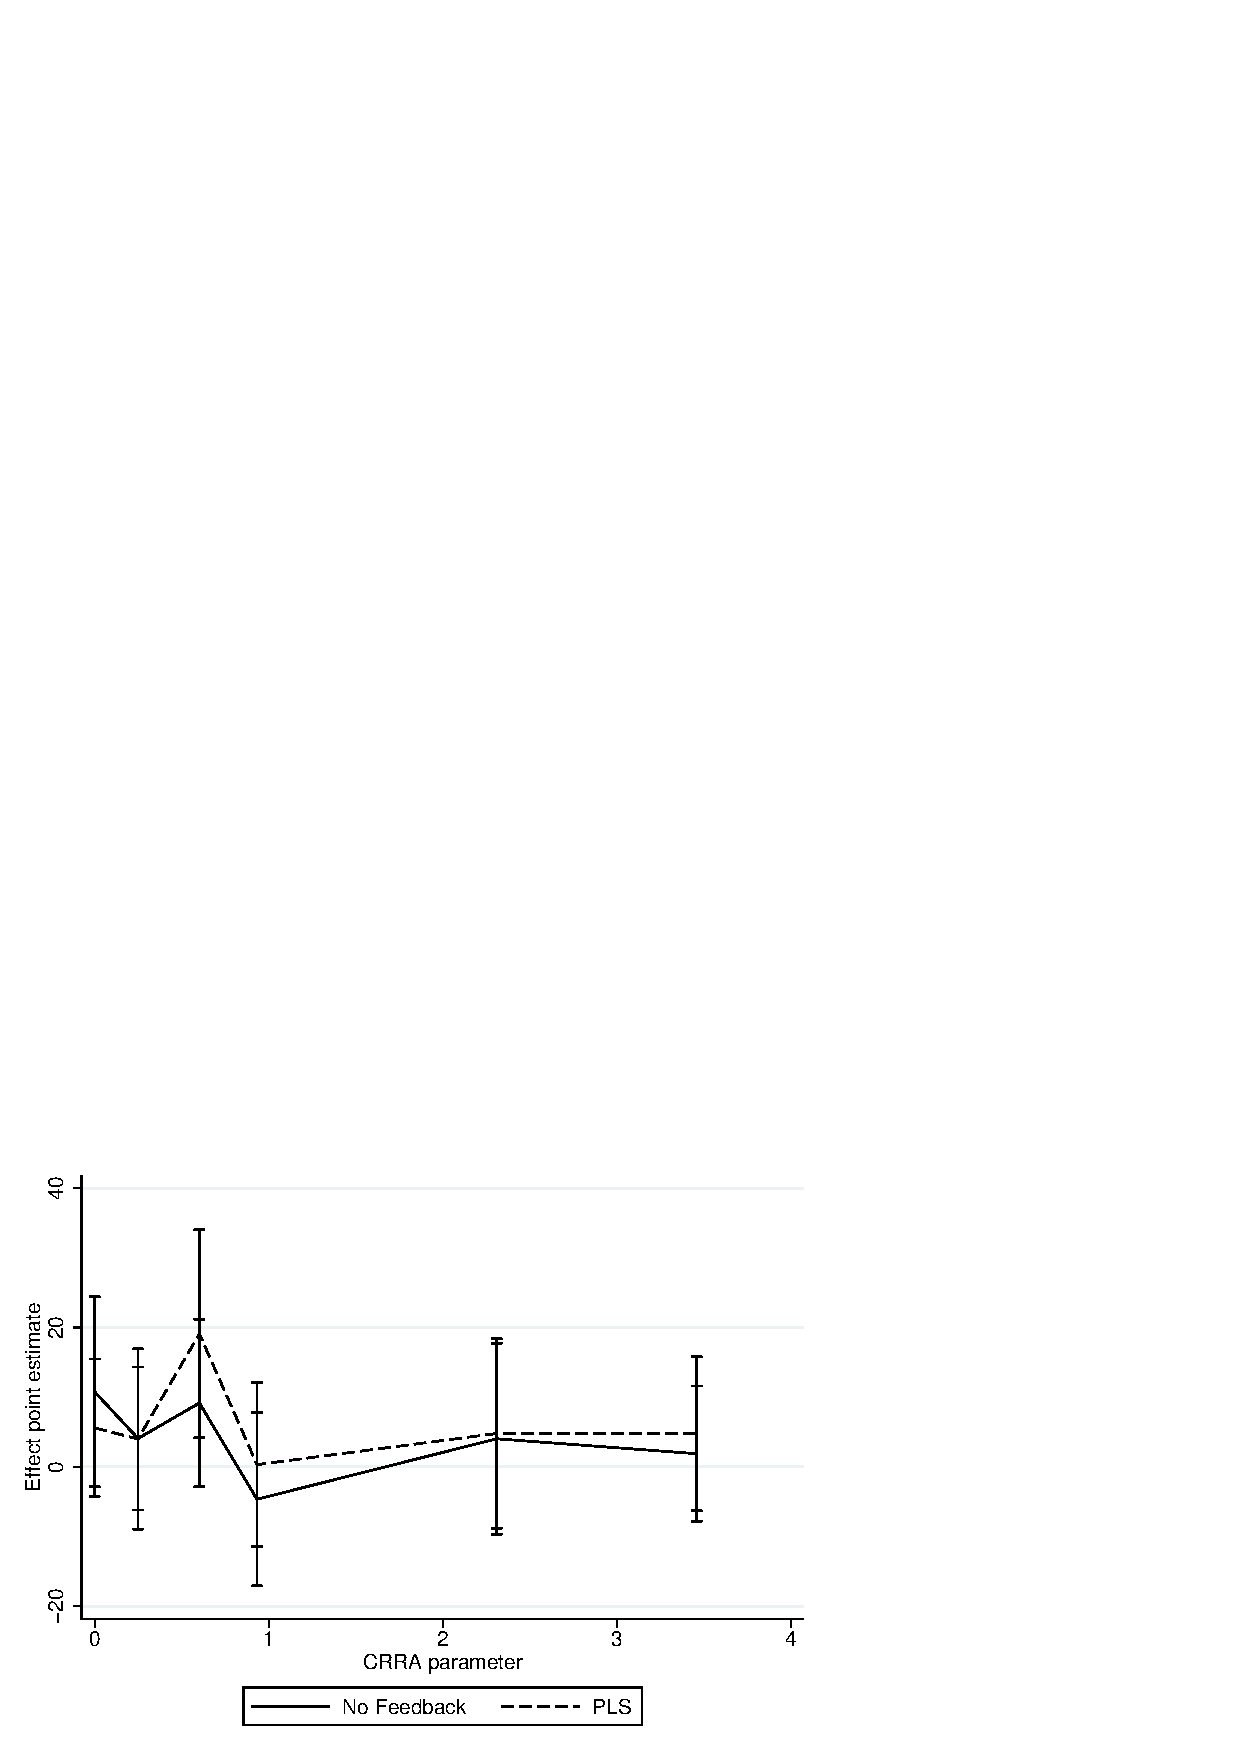
\includegraphics[width=\textwidth]{../../figures/line-mobile_totdepositsbyrisk.pdf}
		\end{figure}

	\clearpage

	\subsection{Savings behavior over project period}

		\begin{figure}[ht]
		\centering
		\caption{Number of daily deposits}
		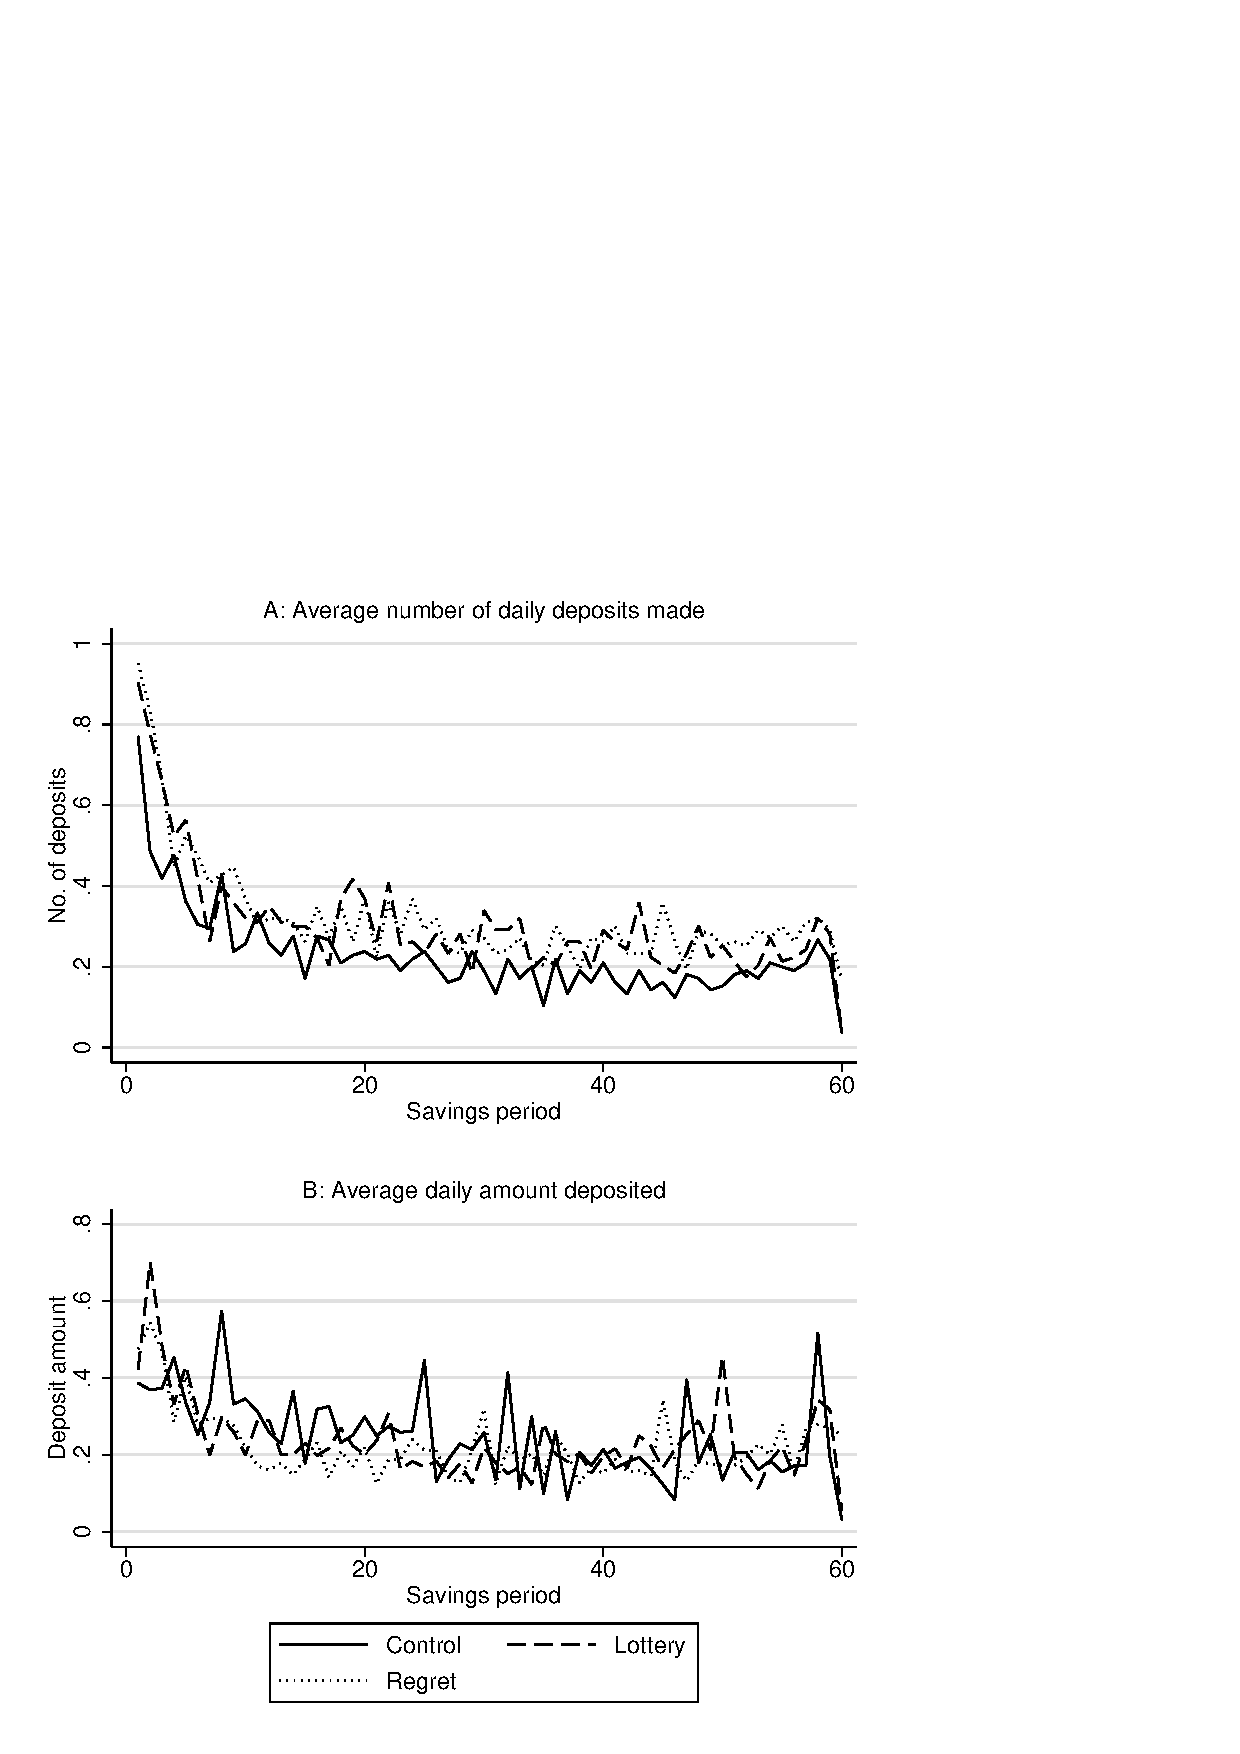
\includegraphics[width=\textwidth]{../../figures/line-deposits.pdf}
		\end{figure}

		\begin{figure}[ht]
		\centering
		\caption{Cumulative number of deposits}
		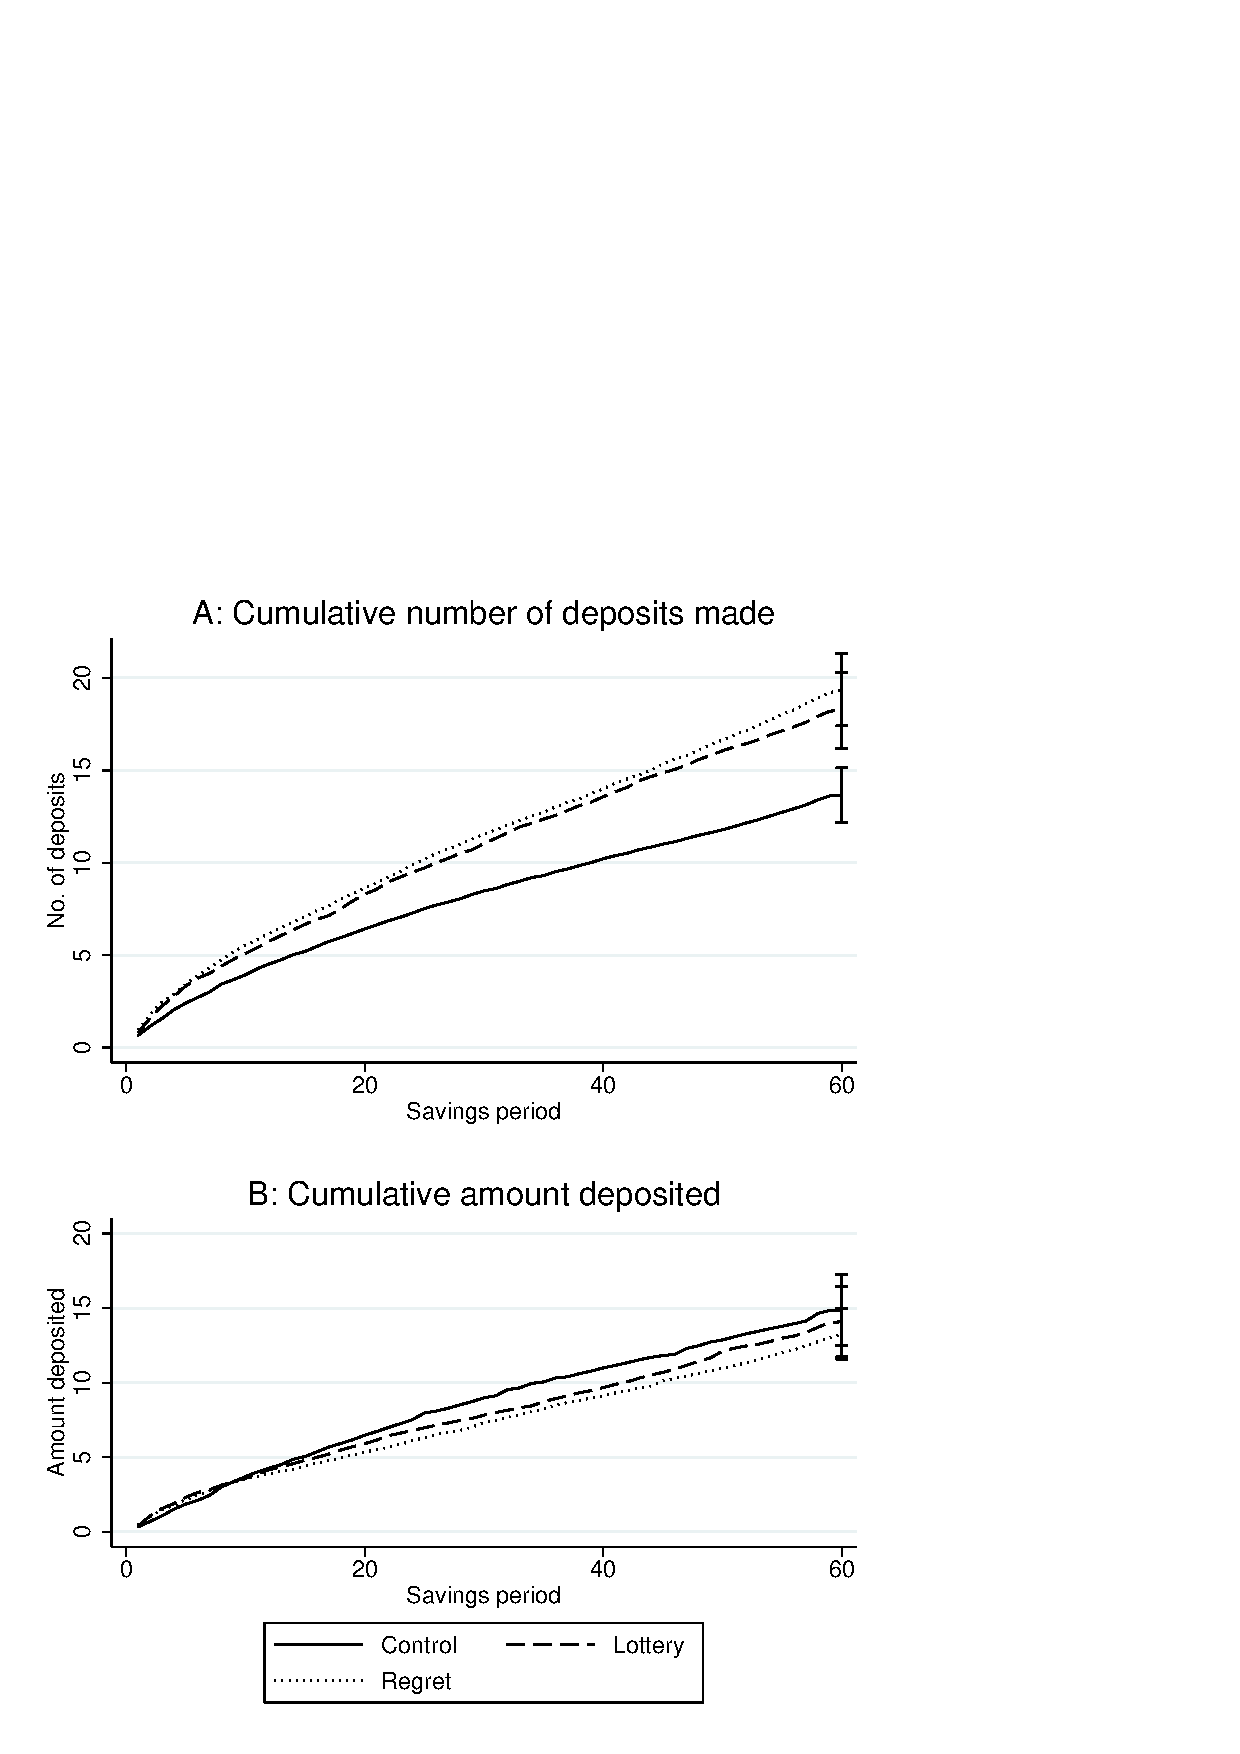
\includegraphics[width=\textwidth]{../../figures/line-cumdeposits.pdf}
		\end{figure}

		\begin{figure}[ht]
		\centering
		\caption{Daily balance averaged over all participants}
		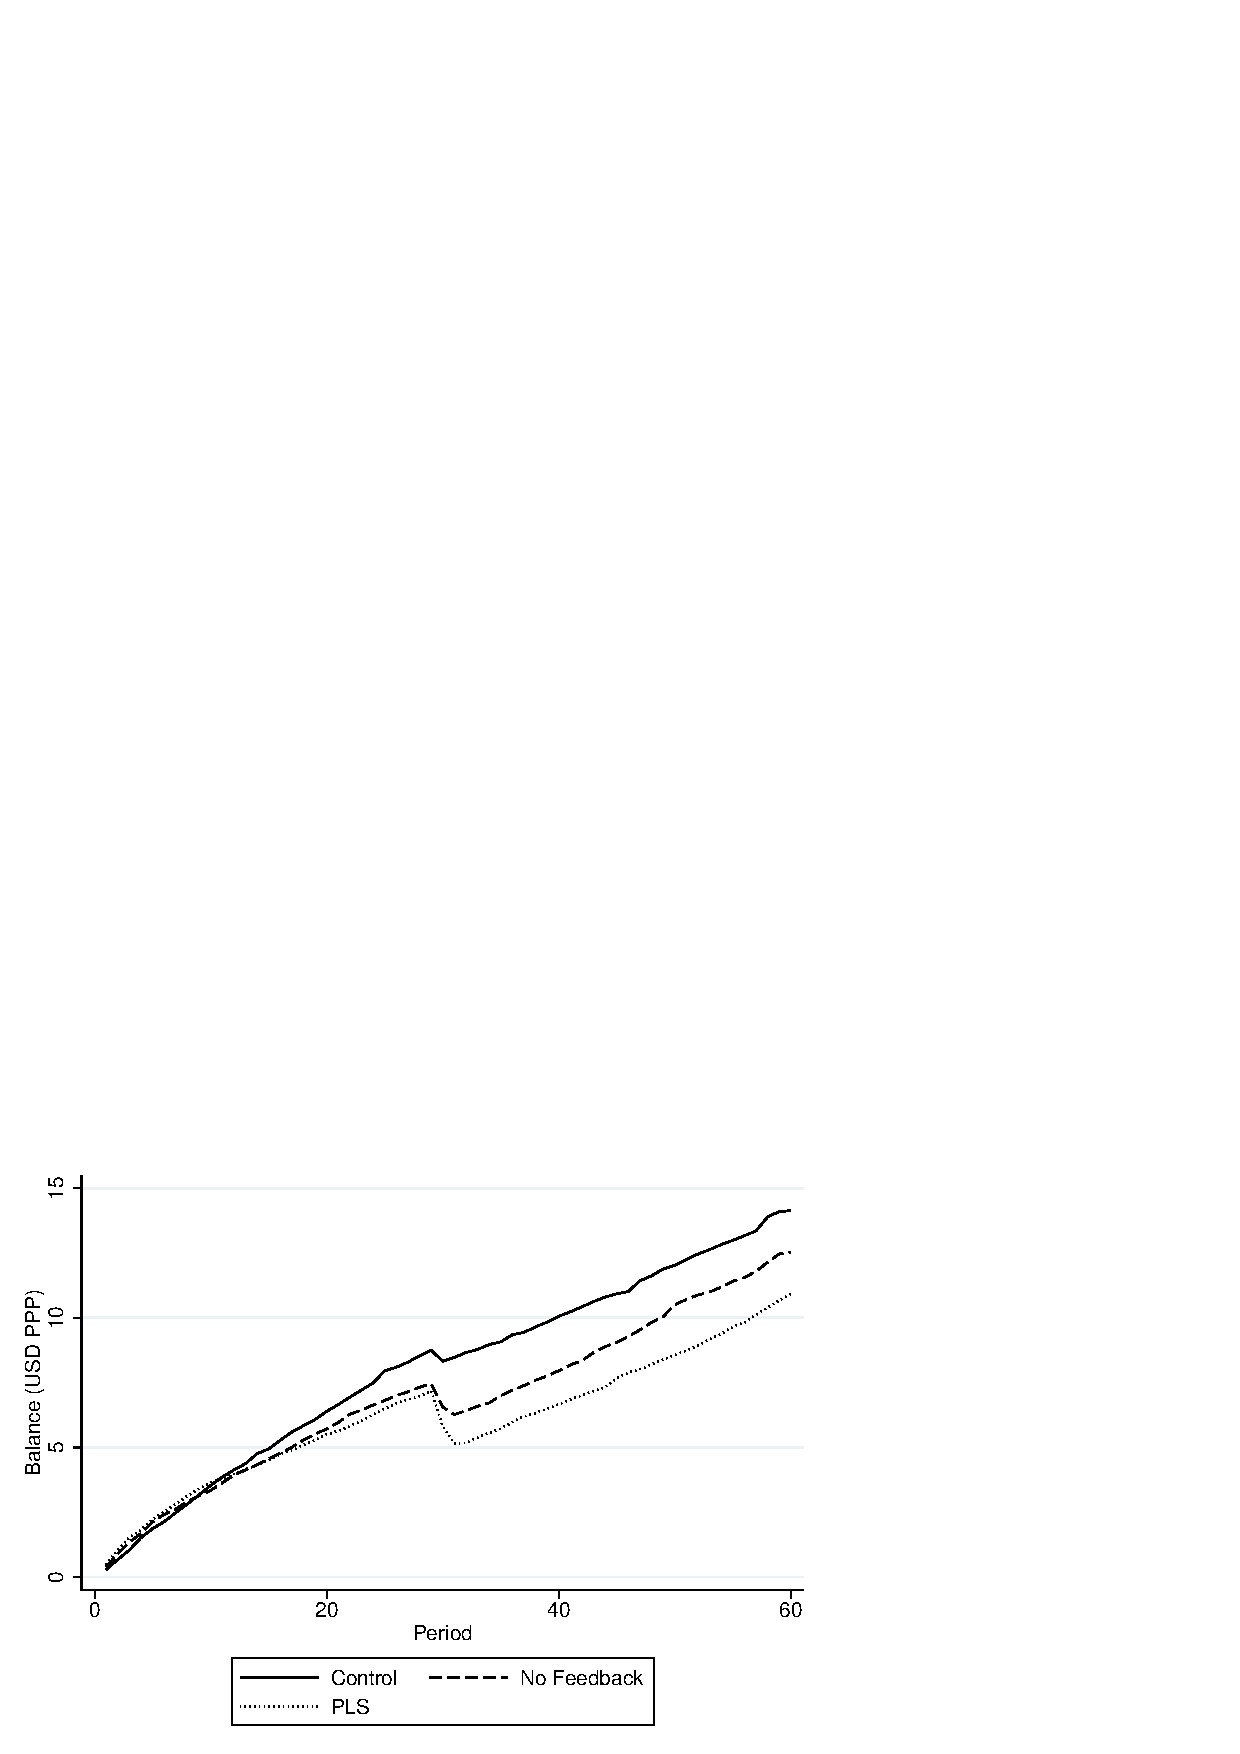
\includegraphics[width=\textwidth]{../../figures/line-balance.pdf}
		\end{figure}

	\clearpage

	\subsection{Panel treatment effects}

        \begin{figure}[ht]
        \centering
        \caption{Effects over time -- Number of deposits}
        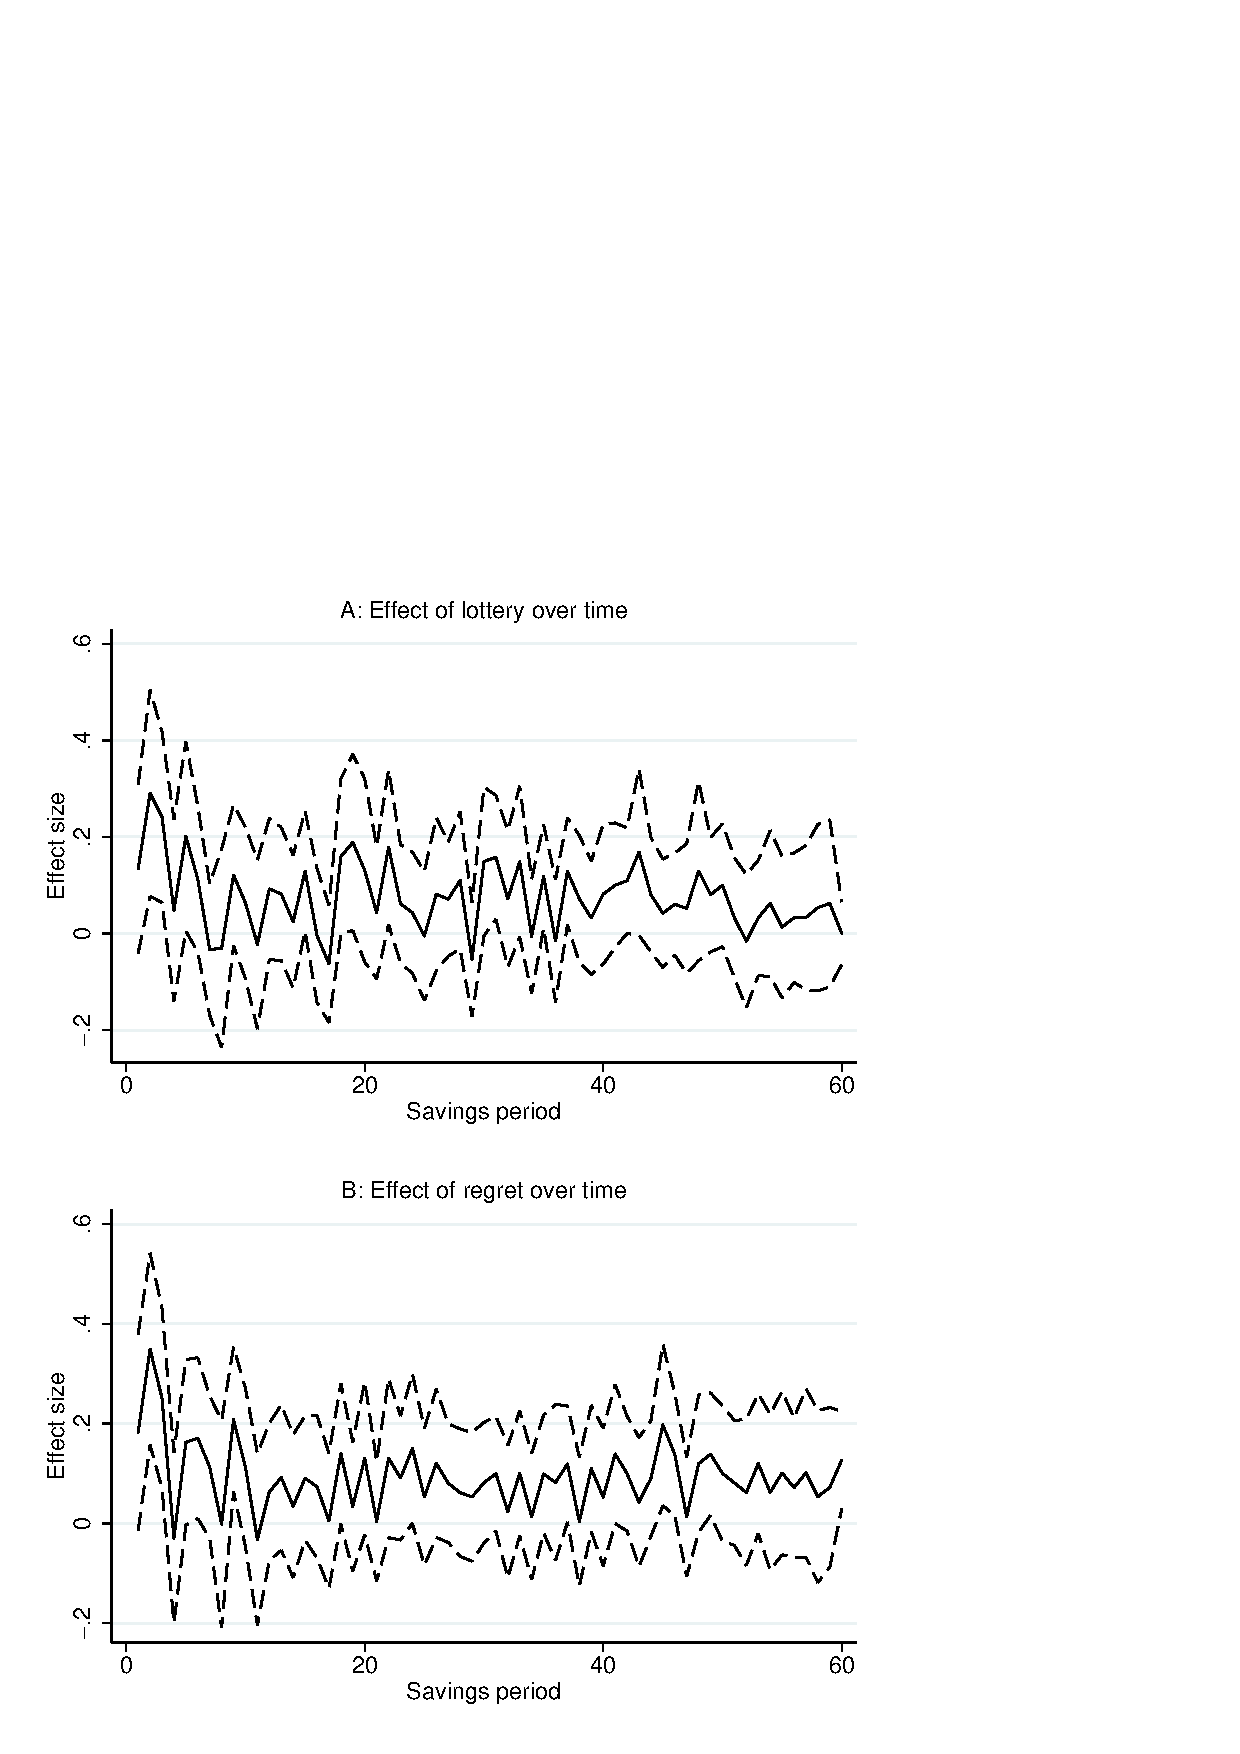
\includegraphics[width=\textwidth]{../../figures/line-timemobile_deposits.pdf}
        \end{figure}

        \begin{figure}[ht]
        \centering
        \caption{Effects over time -- Amount deposited}
        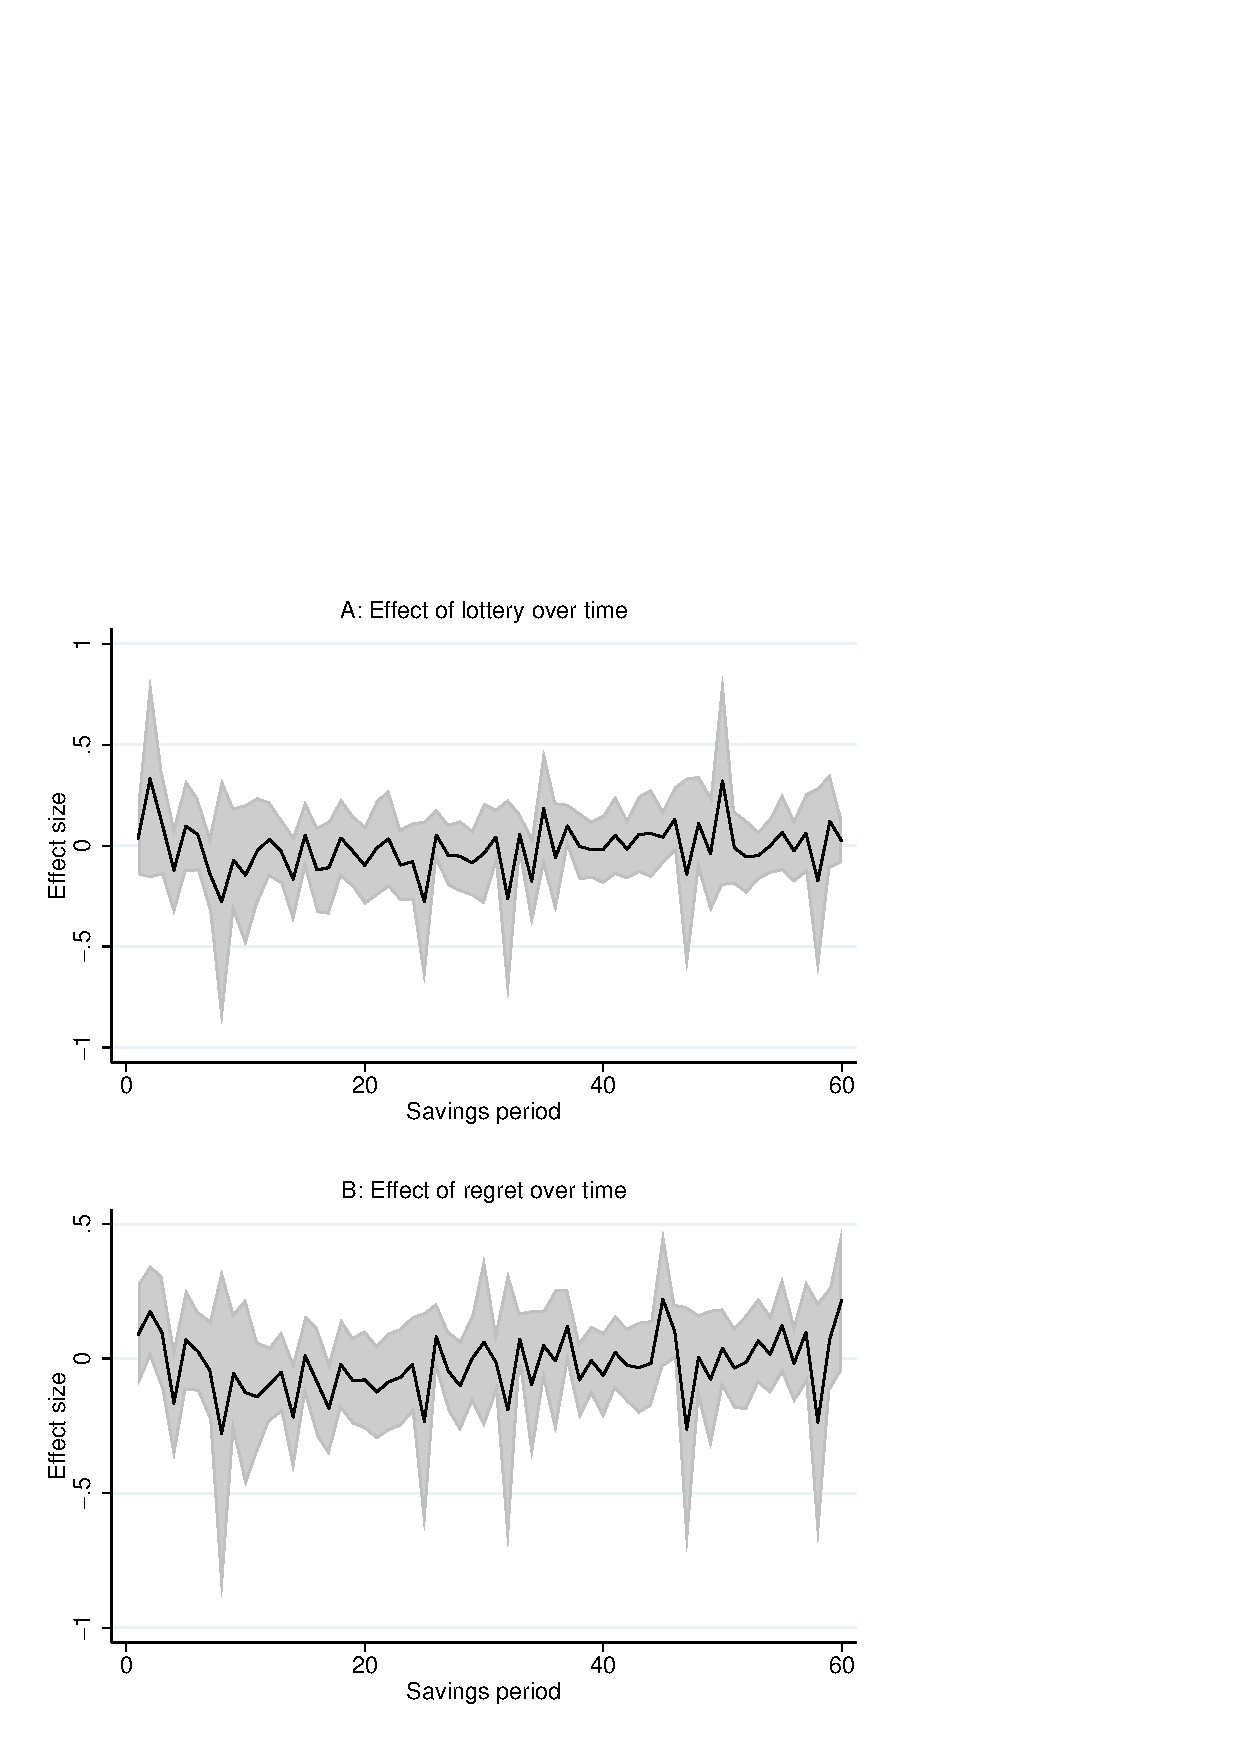
\includegraphics[width=\textwidth]{../../figures/line-timemobile_depositamount.pdf}
        \end{figure}

		% \begin{figure}[ht]
		% \centering
		% \caption{Autoregressive model - Saved on day t}
		% \includegraphics[width=\textwidth]{../../figures/line-ar.pdf}
		% \end{figure}
        %
		% \begin{figure}[ht]
		% \centering
		% \caption{Distributed lag model - Saved on day t}
		% \includegraphics[width=\textwidth]{../../figures/line-dl.pdf}
		% \end{figure}

\end{document}
